
% Tesi D.S.I. - modello preso da
% Stanford University PhD thesis style -- modifications to the report style

\documentclass[12pt,italian,oneside]{book}
\usepackage{tesi}

% CORSO DI LAUREA:
\def\myCDL{Corso di Laurea Magistrale in Informatica}

% TITOLO TESI:
\def\myTitle{
Algoritmi di classificazione basati su vettori di supporto per la produzione di modelli succinti
}

% AUTORE:
\def\myName{Antonio Belotti}
\def\myMat{Matricola 960822}

% RELATORE E CORRELATORE:
\def\myRefereeA{Prof. Dario Malchiodi}
\def\myRefereeB{Prof. Alberto Ceselli}
\def\myRefereeC{Dr. Michele Barbato}

% ANNO ACCADEMICO
\def\myYY{2022-2023}

% Il seguente comando introduce un elenco delle figure dopo l'indice (facoltativo)
\figurespagetrue

% Il seguente comando introduce un elenco delle tabelle dopo l'indice (facoltativo)
\tablespagetrue

% Package di formato
\usepackage[a4paper]{geometry}		% Formato del foglio
\usepackage[italian]{babel}			% Supporto per l'italiano
\usepackage[utf8]{inputenc}			% Supporto per UTF-8
\usepackage[a-1b]{pdfx}             % File conforme allo standard PDF-A (obbligatorio per la consegna)

% Package per la grafica
\usepackage{graphicx}				% Funzioni avanzate per le immagini
\usepackage{subcaption}
%\usepackage{hologo}				% Bibtex logo with \hologo{BibTeX}
%\usepackage{epsfig}				% Permette immagini in EPS
%\usepackage{xcolor}				% Gestione avanzata dei colori


% Package tipografici
\usepackage{amssymb,amsmath,amsthm} % Simboli matematici
%\usepackage{listings}				% Scrittura di codice
% Package ipertesto
\usepackage{url}					% Visualizza e rendere interattii gli URL
%\usepackage[pdfa]{hyperref}		    % Rende interattivi i collegamenti interni
\hypersetup{draft}

\usepackage[italiano,ruled, lined, linesnumbered, longend, onelanguage]{algorithm2e}            % pseudocodice
\DontPrintSemicolon
\SetKw{KwBy}{incrementando di}
\SetKw{KwIn}{in}
\SetKwFor{For}{per}{}{fine per}

\usepackage{booktabs}               % \toprule, \midrule nelle tabelle
\usepackage{hhline}
\usepackage{multirow}
\usepackage{colortbl}

\usepackage[short]{optidef}         % Problemi di ottimizzazione
\usepackage{etoolbox}
\robustify{\label}

\usepackage[italian]{cleveref}  % aggiunge automaticamente anche "capitolo" o "eq." in base a cosa ci si sta riferendo
\crefname{section}{Paragrafo}{Paragrafi}
\Crefname{section}{Paragrafo}{Paragrafi}
\crefname{paragraph}{Capoverso}{Capoversi}
\Crefname{paragraph}{Capoverso}{Capoversi}
\crefname{equation}{Equazione}{Equazioni}
\Crefname{equation}{Equazione}{Equazioni}

\usepackage{setspace}  

\usepackage[toc]{appendix}
\addto\captionsitalian{%
   \renewcommand{\appendixtocname}{Appendici}%
   \renewcommand{\appendixpagename}{Appendici}%
}


% 
% norma di un vettore
\newcommand{\norm}[1]{\|#1\|}

% derivata parziale
\newcommand{\pd}[2]{\frac{\partial{#1}}{\partial{#2}}}

% Vec in grassetto invece che con freccia
\usepackage{ifthen}
\renewcommand{\vec}[1]{%
  \ifthenelse{
    \equal{#1}{\alpha} 
    \OR \equal{#1}{\xi}
    \OR \equal{#1}{\mu}
    \OR \equal{#1}{\beta}
    } % se serve per altri simboli \OR \equal{#1}{\beta}}%
  {\boldsymbol{#1}}%
  {\mathbf{#1}}%
}
%\renewcommand\vec{\mathbf}

%
\newcommand{\sign}{\mathrm{sign}}


\makeindex

\begin{document}

\frontespizio
\beforepreface
    % qui ringraziamenti e prefazione volendo
\afterpreface
    % \listoftables
    % \listoffigures
\frontmatter
    \chapter{Introduzione}
\label{chap:introduzione}
L'ottimizzazione delle prestazioni degli algoritmi di apprendimento automatico è una sfida da sempre presente nella ricerca scientifica e nello sviluppo delle tecnologie basate sull'intelligenza artificiale.

Lo studio e l'utilizzo di modelli efficienti è di particolare importanza in tutti quegli scenari caratterizzati da una scarsità di risorse di calcolo o di memorizzazione.
Se è pur vero che le capacità e la disponibilità dell'hardware sono storicamente da sempre in crescita, è vero anche che permangono (e anzi aumentano) scenari in cui la disponibilità di risorse non è scontata, e per cui l'incremento di tali capacità non è fattibile o conveniente.
Si pensi, per esempio, a tutti quegli oggetti di uso quotidiano ormai dotati di computer di bordo, dagli \emph{smartwatch} ai termostati di casa, la gamma di dispositivi per cui si potrebbe sviluppare ed eseguire un algoritmo intelligente è molto vasta e in crescita.

Tra le molte metodologie di apprendimento automatico più utilizzate, le \emph{support vector machine} (SVM) si sono dimostrate estremamente efficaci nella risoluzione di problemi di classificazione e regressione. 
Tuttavia, per problemi con grandi quantità di dati, i modelli SVM utilizzano un grande numero di \emph{vettori di supporto} (un sottoinsieme di dati di addestramento) per definire una superficie di separazione. 
Questa caratteristica rende i modelli SVM in fase di predizione onerosi in termini di risorse, sia di tempo che di spazio.

Questa tesi si pone l'obiettivo di definire, implementare e valutare sperimentalmente una nuova procedura di addestramento supervisionato per produrre modelli SVM efficienti in grado di utilizzare un numero limitato di vettori di supporto.
In particolare, il lavoro sarà focalizzato su problemi di classificazione binaria, introducendo una procedura di addestramento che consente di impostare \emph{a priori} una quantità massima di vettori di supporto.
Nella fase sperimentale si prova a quantificare il guadagno ottenuto in termini di spazio e l'eventuale perdita di accuratezza nelle previsioni rispetto a un modello SVM classico senza nessuna strategia di contenimento del numero di vettori di supporto.

La tesi è organizzata come segue: nel~\Cref{chap:AI_ML} si introduce il campo dell'apprendimento automatico, descrivendone i problemi tipici e alcuni noti approcci per risolverli; nel~\Cref{chap:SVC} si introducono brevemente i \emph{metodi kernel} e si descrivono in dettaglio i modelli \emph{support vector machine}, in particolare per problemi di classificazione; nel~\Cref{chap:sparse_svc} si espone un'analisi della letteratura relativa all'addestramento di modelli SVM parsimoniosi, per poi descrivere la proposta originale di questa tesi, la modellazione \emph{budgeted SVC}; nel~\Cref{chap:esperimenti} si descrivono gli esperimenti effettuati; si conclude infine con una discussione dei risultati ottenuti e dei possibili sviluppi futuri.
\mainmatter
    \chapter{Apprendimento automatico}\label{chap:AI_ML}
In questo capitolo si introducono i principali problemi e le principali tecniche risolutive nel campo dell'apprendimento automatico.
Nel~\Cref{sec:imparare_dai_dati} si definisce il termine apprendimento automatico; nel~\Cref{sec:tipi_problemi_ml} si categorizzano i principali problemi di apprendimento automatico; nel~\Cref{sec:valutazione_modelli} si descrivono le principali metriche di valutazione dei modelli di apprendimento automatico; nel~\Cref{sec:model_selection} si descrivono le principali tecniche per selezionare i migliori iperparametri per addestrare un modello su un certo \emph{dataset}; nel~\Cref{sec:comuni_approcci_risolutivi} si descrivono i più comuni approcci risolutivi; nel~\Cref{sec:bias_variance_tradeoff} si introduce infine la problematica dell'\emph{overfitting}/\emph{underfitting}; 

\section{Imparare dai dati}\label{sec:imparare_dai_dati}
Risolvere un problema utilizzando un computer richiede un algoritmo, una sequenza di passi da poter implementare ed eseguire. 
Per alcuni problemi sono noti uno o più algoritmi in grado di trovare soluzioni: ordinare una sequenza di numeri, per esempio, è un compito per cui sono noti diversi algoritmi. 
Per alcuni problemi, invece, è possibile identificare i dati in \emph{input}, i dati in \emph{output}, ma non si conosce la procedura per trasformare un \emph{input} in \emph{output}. 
Quali sono i passi per considerare un'\textit{e-mail} come posta indesiderata? 
In caso esistano, sono passi applicabili per ogni casella di posta elettronica? 
Questi criteri cambiano nel tempo o restano fissi? 
Per un essere umano identificare un messaggio come indesiderato è relativamente facile; per una macchina no.

Il fatto che non si possano formalizzare manualmente le caratteristiche che rendono una \emph{e-mail} indesiderata, non vuol dire che queste caratteristiche non esistano. 
Ci sono, ma sono ``nascoste'' tra i dati.
L'apprendimento automatico è una branca dell'intelligenza artificiale che studia tutti quegli algoritmi in grado di analizzare insiemi (più o meno grandi) di dati per poi produrre un modello capace di eseguire delle predizioni soddisfacenti su dati mai visti prima. 
Oltre alla caratteristica di risolvere compiti che richiedono intelligenza, le varie tecniche di apprendimento automatico si prestano a un continuo miglioramento, adattando i modelli nel tempo.
Per esempio, i sistemi in grado di identificare posta indesiderata possono essere aggiornati, riaddestrati o raffinati nel tempo con l'aggiunta di nuovi esempi di messaggi segnalati dall'utente come indesiderati.

Lo studio dei modelli di apprendimento automatico si concentra su due compiti principali: definire procedure di addestramento e definire procedure di inferenza. 
In genere l'obiettivo principale è quello di costruire dei modelli efficaci in grado di eseguire predizioni affidabili secondo delle metriche definite in base al problema trattato. 
In altri scenari, caratterizzati da una scarsità di risorse computazionali o temporali, è invece necessario enfatizzare l'efficienza del modello in fase di predizione, idealmente senza sacrificare buone capacità di inferenza.

Creare dei modelli efficienti in fase di predizione ha un potenziale riscontro di efficienza anche in termini energetici.
Ridurre le dimensioni e i requisiti computazionali di un modello si traduce infatti in meno cicli di calcolo da eseguire, e di conseguenza in un minor consumo di energia.
Quantificare il risparmio energetico ottenuto con l'utilizzo di modelli efficienti rispetto a modelli tradizionali non è un compito facile ma è di assoluta attualità.

\section{Problemi e algoritmi di apprendimento automatico supervisionato}\label{sec:tipi_problemi_ml}
Ipotizziamo che esista la funzione $f:\mathcal{X}\rightarrow\mathcal{Y}$ che associa alle istanze $x \in \mathcal{X}$ di un problema le corrispondenti soluzioni $y \in \mathcal{Y}$, ma che tale funzione sia ignota. 
Un algoritmo di apprendimento automatico supervisionato costruirà un modello $h:\mathcal{X}\rightarrow\mathcal{Y}$ che approssima $f$ a partire da un insieme di dati di addestramento $\mathcal{S}=\{(x_i, y_i), i=1,\dots,m\}$, dove $\mathcal{S} \subset \mathcal{X} \times \mathcal{Y}$.
Semplificando, si può pensare a $\mathcal{X} = \mathbb{R}^d$, quindi ogni dato in \emph{input} è un vettore $\Vec{x}_i=[x_i^{(1)},\dots,x_i^{(d)}]$.
Ogni componente dei vettori di \emph{input} è chiamato \emph{attributo}.
I dati $y_i \in \mathcal{Y}$ sono chiamati \emph{etichette}; si indicano invece le predizioni di un modello come $\hat{y} = h(\Vec{x})$. 

Si parla di apprendimento supervisionato~\cite{elements-of-statistical-learning} perché l'algoritmo di apprendimento richiede la presenza delle etichette $y_i$ in fase di addestramento.
Esiste un'altra categoria di algoritmi, gli algoritmi di apprendimento non supervisionato~\cite{unsupervised_learning}, che trattano problemi in cui le etichette non sono note.
Si menziona per completezza l'esistenza di una terza categoria, l'apprendimento per rinforzo~\cite{reinforcement_learning}, che include algoritmi che cercano di costruire degli ``agenti intelligenti'' che identificano la miglior sequenza di operazioni seguendo dei meccanismi di ricompensa e penalizzazione. 
Gli agenti stessi possono avere un effetto nell'ambiente in cui stanno operando, modificando la scelta delle operazioni da compiere.

Una possibile suddivisione dei problemi risolvibili con algoritmi di apprendimento supervisionato è quella in problemi di classificazione e problemi di regressione.
Per un problema di \emph{regressione} le etichette assumono valori quantitativi, mentre per un problema di \emph{classificazione} le etichette assumono valori che identificano una o più categorie. 
Predire il prezzo di vendita di un immobile a partire dalle alcune sue caratteristiche è, per esempio, un problema di regressione, perché il prezzo di vendita è una quantità;
identificare se un immagine contiene un gatto oppure no è invece un problema di classificazione, perché la predizione è un valore associato ad una categoria, per esempio $0$ per ``vero'' e $1$ per ``falso''.

I problemi di classificazione sono a loro volta ulteriormente suddivisi in base alla forma e al significato delle etichette. Si identificano i casi seguenti.
\begin{itemize}
    \item Problemi di classificazione binaria: la predizione è una sola etichetta tra due possibili valori, per esempio $\hat{y} \in \{0,1\}$. A prescindere dal valore numerico utilizzato, le due possibili classi sono chiamate classe positiva e classe negativa.
    \item Problemi di classificazione multi-classe: la predizione $\hat{y}$ è un vettore di $k$ componenti, ognuno a indicare una possibile classe.
    Tra tutte le possibili classi, una predizione ne identifica solo una. 
    In alcuni casi, a seconda del modello utilizzato, la predizione può essere interpretata come una distribuzione di probabilità.  
    \item Problemi di classificazione multi-etichetta: come per problemi di classificazione multi-classe, la predizione $\hat{y}$ è un vettore di $k$ componenti, ognuno a indicare una possibile classe, con la differenza che in questo caso più di un'etichetta può essere identificata. 
\end{itemize}

Anche per problemi di regressione, nel caso in cui i valori da predire siano più di uno, si parla di regressione multi-etichetta.

I principali problemi risolti con algoritmi di apprendimento non supervisionato sono invece descritti nel seguente elenco.
\begin{itemize}
    \item \emph{Clustering}~\cite{elements-of-statistical-learning}: lo scopo è quello di suddividere un insieme di dati non etichettati in gruppi sulla base di criteri di similarità o distanza geometrica.
    \item Riduzione della dimensionalità~\cite{elements-of-statistical-learning}: lo scopo è quello di trasformare i dati originali in uno spazio con meno dimensioni senza perdita significativa di informazione.
    \item Regole di associazione~\cite{elements-of-statistical-learning}: lo scopo è quello di estrarre dai dati delle relazioni significative nella forma di implicazione ``se $x$ allora $y$''.
\end{itemize}

Ricapitolando, l'obiettivo di una procedura di addestramento automatico è quello di approssimare una funzione ignota $f$ con un modello $h$ in modo che l'errore dovuto all'approssimazione sia accettabile.
La valutazione della bontà di un modello è una parte fondamentale del processo.
In base al tipo di problema, al tipo di dati, all'ambito di applicazione concreto del modello, si utilizzano metriche e tecniche diverse.
Questi aspetti saranno approfonditi nei~\Cref{sec:valutazione_modelli,sec:model_selection}.

Per concludere questo paragrafo è opportuno definire i termini parametro e iperparametro.
Un \emph{parametro} è una variabile di un modello il cui valore è ottimizzato dall'algoritmo di apprendimento nel processo di creazione del modello stesso. 
Un \emph{iperparametro} è invece una variabile il cui valore deve essere fissato dal programmatore prima di eseguire l'algoritmo di apprendimento, che è influenzato dal valore scelto.

\section{Valutazione dei modelli}\label{sec:valutazione_modelli}
Nel campo dell'apprendimento automatico è di fondamentale importanza utilizzare delle metriche per misurare l'efficacia dei modelli sia durante la fase di addestramento che durante la fase di utilizzo su dati mai visti.
A prescindere dalla metrica utilizzata, la bontà di un modello è in genere misurata su un insieme di dati di \emph{test}, ovvero un sottoinsieme dei dati disponibili utilizzato solo ed esclusivamente per questo scopo.
L'insieme di \emph{test} simula un insieme di dati nuovi mai visti dal modello.
Per una valutazione significativa è necessario un insieme di \emph{test} significativo, composto da un numero sufficiente di elementi e con una distribuzione di etichette il più fedele possibile al corrispettivo insieme di addestramento.
La scelta della composizione dell'insieme di \emph{test} è centrale, esattamente come la scelta della composizione dei dati di addestramento.
In generale, la qualità e la quantità dei dati utilizzati in un qualsiasi processo di apprendimento automatico è di fondamentale importanza e influenza direttamente la bontà dei modelli creati.

Generalmente, l'approccio più semplice per valutare un modello prevede di dividere l'insieme di dati disponibile in due parti: un insieme per l'addestramento e un insieme di \emph{test}. 
Questo metodo può essere applicato quando la dimensione del \emph{dataset} di partenza consente di creare delle partizioni sufficientemente grandi sia per addestrare il modello che per valutarlo.
Nei casi in cui la dimensione ridotta del \emph{dataset} di partenza non garantisca queste possibilità, è necessario considerare altri metodi per addestrare e valutare un modello, per esempio \emph{repeated holdout} o \emph{cross validation}, descritti nei prossimi paragrafi.

Ipotizzando di avere a disposizione un insieme di \emph{test} di qualità, ci sono altri criteri che guidano la valutazione di un modello.
La quantità di dati disponibili è un fattore che influisce anche sulla tipologia di modello utilizzabile.
Alcuni modelli richiedono grandi quantità di dati per essere addestrati, mentre altri modelli sono più adatti per piccoli \emph{dataset}. 

Il tipo di modello utilizzato e il tipo di problema trattato guida la scelta di una metrica adatta per valutarne la bontà: per problemi di classificazione, ad esempio, ha senso utilizzare il numero di predizioni corrette in rapporto al numero di predizioni totali; per problemi di regressione, invece, non è possibile utilizzare lo stesso criterio perché le predizioni sono quantitative e non è semplicemente possibile contare il numero di predizioni corrette. 

\subsection{Metriche per modelli di classificazione}\label{sec:metriche_valutazione_modelli}
Considerando per semplicità un problema di classificazione binaria, si definiscono:
\begin{itemize}
    \item TP il numero di predizioni correttamente identificate nella classe positiva,
    \item TN il numero di predizioni correttamente identificate nella classe negativa,
    \item FP il numero di predizioni erroneamente identificate nella classe positiva,
    \item FN il numero di predizioni erroneamente identificate nella classe negativa.
\end{itemize}
Queste quantità sono spesso organizzate in una matrice, chiamata matrice di confusione. 
Si tratta sostanzialmente di una tabella in cui le righe identificano le predizioni e le colonne identificano le etichette reali. 
Viene riportato in~\Cref{tab:matrice_confusione} un esempio di matrice di confusione per un classificatore binario ipotetico che identifica o meno la presenza di una malattia a partire da un referto preso in \emph{input}.
\begin{table}[h]
    \centering
    \begin{tabular}{l|l|c|c|}
        \multicolumn{2}{c}{}&\multicolumn{2}{c}{Etichette}\\
        \cline{3-4}
        \multicolumn{2}{c|}{} & Positive & Negative\\
        \cline{2-4}
        \multirow{2}{*}{Predizioni}& Positive & 1 (TP) & 1 (FP) \\
        \cline{2-4}
        & Negative & 8 (FN) & 90 (TN) \\
        \cline{2-4}
    \end{tabular}
    \caption[Esempio di matrice di confusione per un problema di classificazione binaria]{Esempio di matrice di confusione per un problema di classificazione binaria, da \protect\footnotemark.}
    \label{tab:matrice_confusione}
\end{table}

\footnotetext{\url{https://developers.google.com/machine-learning/crash-course/classification/accuracy?hl=en}}

I paragrafi successivi descrivono le metriche tipicamente utilizzate per valutare un classificatore binario.

\subsubsection{Accuratezza} L'\emph{accuratezza} è una delle metriche principali utilizzate per problemi di classificazione, ed è calcolata come:
\begin{equation*}
    \textrm{\emph{Accuratezza}} = \frac{\text{Numero di predizioni corrette}}{\text{Numero di predizioni totali}} = \frac{\text{TP} + \text{TN}}{\text{TP} + \text{TN} + \text{FP} + \text{FN}}.
\end{equation*}
Questa metrica può dare una prima indicazione delle capacità di un classificatore ma può essere poco significativa a seconda del problema considerato, perché non quantifica la distribuzione delle predizioni corrette né la distribuzione di quelle errate.
Nell'esempio in~\Cref{tab:matrice_confusione} l'accuratezza ha valore $0.91$, il che sembrerebbe indicare un buon classificatore.
Per il problema oggetto dell'esempio però, questo valore è ingannevole, dato che 8 pazienti sarebbero classificati dal modello come in salute quando invece non lo sono: questi 8 falsi negativi hanno un costo molto alto rispetto al costo che si avrebbe nel commettere l'errore opposto. 
Predire un paziente come sano quando in realtà è malato è molto costoso perché indurrà il paziente a non curarsi risultando in un peggioramento della malattia. 
Al contrario, predire un paziente sano come malato, non è particolarmente grave, perché risulta sostanzialmente in un eccesso di precauzione: si potrà sempre intervenire in seguito con ulteriori esami per confermare o smentire la diagnosi.

Considerando invece un altro scenario, in cui un'azienda che riceve un numero molto elevato di candidature vuole predire se una persona da assumere sarà un buon lavoratore oppure no, il costo degli errori è diverso. In questo caso, un falso negativo non è particolarmente costoso: è meglio rifiutare un candidato valido (tra i molti disponibili) piuttosto che correre il rischio di assumere un candidato non valido. 

L'accuratezza non è sufficiente per valutare questi dettagli ed è per questo che sono state introdotte altre metriche, in particolari quelle descritte nei paragrafi successivi.

\subsubsection{Precisione} La \emph{precisione}, calcolata come
\begin{equation*}
    \textrm{\emph{Precisione}} = \frac{\text{TP}}{\text{TP} + \text{FP}},
\end{equation*}
è una misura di quanti degli esempi predetti positivi sono effettivamente positivi.
Un modello che predice correttamente tutti gli esempi positivi avrà un valore di precisione uguale ad $1$.
Nell'esempio in~\Cref{tab:matrice_confusione} il valore di precisione è $0.5$: quando un paziente è segnalato come ammalato, lo è effettivamente nella metà dei casi.

\subsubsection{Sensibilità} La \emph{sensibilità}, calcolata come 
\begin{equation*}
    \textrm{\emph{Sensibilità}} = \frac{\text{TP}}{\text{TP} + \text{FN}},
\end{equation*}
è una misura di quanti degli effettivi veri positivi sono identificati come tali dal modello.
Nell'esempio in~\Cref{tab:matrice_confusione} il valore di sensibilità è $0.11$: tra tutti gli effettivi pazienti ammalati, il modello ne identifica correttamente l'$11\%$.


\subsubsection{F1} 
Siccome è facile ottenere un'alta precisione a discapito di una bassa sensibilità e viceversa, ottimizzare una sola di queste due metriche può portare a scarsi risultati complessivi.
La metrica F1, calcolata come 
\begin{equation*}
    \textrm{\emph{F1}} = \frac{2(\text{\emph{Precisione}} \times \text{\emph{Sensibilità}})}{\text{\emph{Precisione}} + \text{\emph{Sensibilità}}} = \frac{2\text{TP}}{2\text{TP}+ \text{FP}+ \text{FN}},
\end{equation*}
è la media armonica tra precisione e sensibilità. Questa metrica assume un valore alto quando sia precisione che sensibilità sono molto alte.

\subsection{Metriche per problemi di regressione}
Per dare un'idea di come la valutazione dei modelli di regressione sia diversa rispetto alla valutazione dei modelli di classificazione, si riportano in questo paragrafo alcune comuni metriche per problemi di regressione. 

\subsubsection{Mean squared error (MSE)}
La metrica MSE, calcolata come
\begin{equation*}
    \textrm{MSE} = \frac{1}{m} \sum_{i=1}^{m} (y_i - \hat{y}_i)^2,
\end{equation*}
dove $m$ è il numero di elementi considerati, è la media della differenza tra predizione ed etichetta attuale elevata al quadrato. 
Elevare $y_i - \hat{y}_i$ al quadrato evita che la somma di quantità negative risulti in un valore vicino a zero, indicando erroneamente un modello complessivamente buono, quando invece gli errori singoli potrebbero essere considerevoli.

\subsubsection{Root mean squared error (RMSE)}
La metrica RMSE, calcolata come
\begin{equation*}    
    \textrm{RMSE} = \sqrt{\frac{1}{m} \sum_{i=1}^{m} (y_i - \hat{y}_i)^2},
\end{equation*}
dove $m$ è il numero di elementi considerati, non è altro che la radice quadrata della metrica MSE, il che risulta in una metrica con la stessa unità di misura dei dati di addestramento. 

\subsubsection{Mean absolute error (MAE)}
La metrica MAE, calcolata come
\begin{equation*}    
    \textrm{MAE} = \frac{1}{m} \sum_{i=1}^{m} |y_i - \hat{y}_i|,
\end{equation*}
dove $m$ è il numero di elementi considerati, diminuisce il peso degli errori gravi rispetto alla metrica MSE, evidenziando in misura minore gli scarti maggiori di uno.
Come la metrica RMSE, anche MSE ha la stessa unità di misura dei dati di addestramento. 

\subsection{k-fold cross validation}
La procedura $k$\emph{-fold cross validation} è una tecnica per ottenere delle stime robuste di una metrica, valutandola diverse volte su diversi insiemi di \emph{test}.
Il termine $k$ identifica un iperparametro che determina il numero di valutazioni effettuate.
Il funzionamento è il seguente:
\begin{enumerate}
    \item Si suddividono casualmente i dati in $k$ sottoinsiemi, chiamati \emph{fold}.
    \item Per $k$ volte, si sceglie un \emph{fold} da utilizzare come \emph{test} mentre i restanti $k-1$ vengono utilizzati per addestrare un modello. Per ogni iterazione si valuta la metrica sul \emph{fold} di test.
    \item Come stima della metrica, si calcola la media delle $k$ valutazioni effettuate precedentemente.
\end{enumerate}
La~\Cref{fig:kfoldcv} mostra graficamente un esempio delle suddivisioni effettuate dal metodo.
\begin{figure}
    \centering
    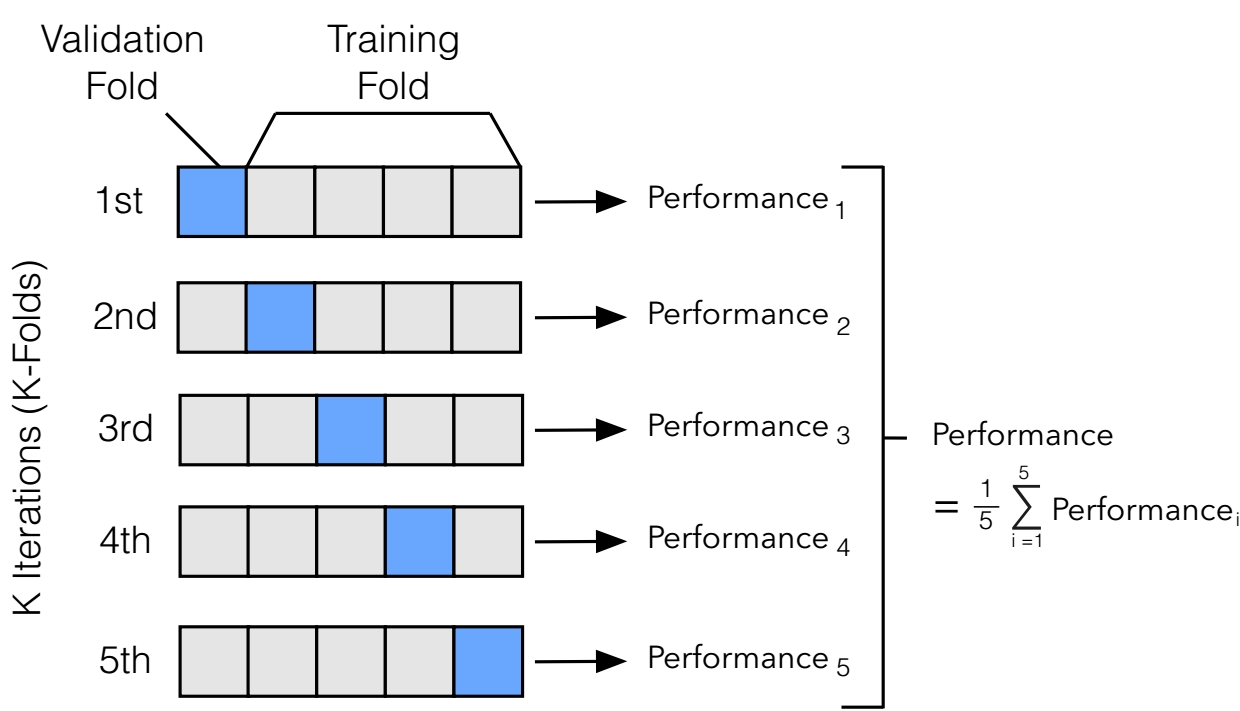
\includegraphics[width=0.7\linewidth]{img/kfoldCV.jpg}
    \caption[Esempio \emph{5-fold cross-validation}.]{Tratto da~\cite{model_evaluation}. Esempio di come \emph{5-fold cross validation} suddivide i dati di addestramento disponibili in 5 parti, utilizzandole tutte una volta come \emph{test} (i riquadri blu).}
    \label{fig:kfoldcv}
\end{figure}
Si parla di \emph{stratified k-fold cross-validation} quando la procedura mantiene la proporzione delle etichette originali nel creare le diverse suddivisioni.


\section{Selezione dei modelli}\label{sec:model_selection}
L'addestramento di un modello di apprendimento automatico richiede il più delle volte la scelta di un valore per alcuni iperparametri. 
Nel caso dei modelli \emph{k-nearest neighbours} (descritti in seguito nel~\Cref{sec:ml:knn}), per esempio, è necessario fissare un valore per il parametro $k$. 
La scelta di questi eventuali iperparametri è di assoluta importanza, ma non esiste una regola generica ed automatica per fissare a priori un valore soddisfacente. La scelta dei valori potrebbe dipendere da tanti fattori, come per esempio dalle caratteristiche dei dati a disposizione, oppure dagli obiettivi desiderati (per esempio potrebbe essere preferibile un modello che genera pochissimi falsi negativi a scapito di più falsi positivi).
In genere, si utilizzano dei criteri o degli algoritmi per selezionare le migliori combinazioni di iperparametri per il problema da risolvere: questa fase nel processo di creazione di un modello di addestramento automatico è chiamata \emph{model selection}.
Le tecniche di \emph{model selection} richiedono molteplici esecuzioni dell'algoritmo di addestramento e altrettante valutazioni su un insieme di dati che non può però essere l'insieme di \emph{test}, dato che è riservato per la valutazione finale di un modello. 
L'insieme di \emph{test} simula dei dati mai visti dal modello per stimare la bontà di generalizzazione e non può essere utilizzato per aggiustare gli iperparametri.
In caso lo fosse si verificherebbe lo scenario chiamato come \emph{data leakage}, ovvero l'utilizzo durante l'addestramento di informazioni che non dovrebbero essere usate per non falsare la bontà del modello.
Si descrivono in questo paragrafo le principali tecniche di \emph{model selection}, mentre in~\cite{model_evaluation} si può trovare una descrizione esaustiva.

I prossimi due paragrafi descrivono rispettivamente le tecniche di identificazione dei migliori valori per gli iperparametri e la problematica del \emph{bias} pessimistico.

\subsubsection{Combinazioni di valori degli iperparametri}
I possibili valori per ogni iperparametro sono definiti in una griglia di iperparametri.
In base ai possibili valori che vengono provati nella procedura di selezione del miglior modello, si identificano diverse strategie di \emph{grid search}, ovvero procedure per provare le varie combinazioni di parametri, tra cui le seguenti.
\begin{itemize}
    \item \emph{Grid search} esaustiva, in cui si provano tutte le possibili combinazioni di iperparametri. \`E la strategia più semplice ma anche la più costosa dal punto di vista computazionale, perché è sostanzialmente una ricerca a forza bruta.
    \item \emph{Randomized grid search}~\cite{random_grid_search}, in cui si selezionano casualmente dei sottoinsiemi delle possibili combinazioni di iperparametri da provare. Il risultato potrebbe variare tra diverse esecuzioni e non c'è la garanzia di trovare la miglior combinazione tra i valori della griglia.
    Ciò nonostante questa strategia può comunque fornire un buon risultato e rimane una buona opzione da considerare nei casi in cui una ricerca esaustiva non sia fattibile. 
\end{itemize}


\subsubsection{Bias pessimistico} Il termine \emph{bias} pessimistico indica che la valutazione delle capacità di generalizzazione effettuata su un sottoinsieme dei dati disponibili possa essere troppo pessimistica rispetto alle capacità che si sarebbero potute ottenere addestrando il modello sull'intero insieme di dati~\cite{model_evaluation}.
Purtroppo, utilizzare tutti i dati disponibili per addestrare il modello renderebbe inaffidabile qualsiasi valutazione effettuata con gli stessi (a causa del \emph{data leakage}); si preferisce di solito una valutazione pessimistica che una ottimistica.


\subsection{Triplo hold-out}
Si è già discusso di come il \emph{dataset} di \emph{test} non possa essere utilizzato per trovare i migliori iperparametri per un modello.
Un primo approccio è quello di suddividere in modo leggermente diverso l'insieme totale dei dati a disposizione, prevedendo 3 sottoinsiemi, descritti nell'elenco seguente.
\begin{itemize}
    \item Insieme di addestramento (\emph{train set}): utilizzato per addestrare i modelli.
    \item Insieme di validazione (\emph{validation set}): utilizzato per valutare i modelli con lo scopo di definire i migliori iperparametri.
    \item Insieme di \emph{test} (\emph{test set}): utilizzato in ultima battuta per stimare l'errore di generalizzazione.
\end{itemize}
Questa suddivisione in tre parti è chiamata \emph{triplo hold-out}.

La selezione di un insieme di validazione è critica tanto quanto la selezione dell'insieme di \emph{test}.
La procedura di selezione del miglior modello procede applicando i passi seguenti.
\begin{enumerate}
    \item Per ogni combinazione di parametri che si desidera valutare, si addestra un modello sull'insieme di addestramento e lo si valuta sull'insieme di validazione.
    \item Si utilizzano gli iperparametri che al passo precedente hanno generato il modello più performante per addestrare un nuovo modello sull'unione dei dati di addestramento con i dati di validazione, cercando così di ridurre il \emph{bias} pessimistico.
    \item Si misura la bontà di questo ultimo modello sui dati di \emph{test}.
\end{enumerate}

\subsection{Hold-out e cross-validation}
Estendendo l'approccio presentato nel paragrafo precedente, è possibile integrare la tecnica di \emph{cross-validation} nel processo di selezione dei migliori iperparametri, utilizzando il procedimento seguente.
\begin{enumerate}
    \item Si suddividono i dati in due insiemi: addestramento e \emph{test}.
    \item Per ogni combinazione di parametri che si desidera valutare, si addestra un modello sull'insieme di addestramento utilizzando \emph{cross-validation} per valutarne la bontà.
    \item Si selezionano gli iperparametri che hanno generato al passo precedente il modello più performante, e si addestra un nuovo modello sull'intero insieme di addestramento.
    \item Si misura infine sui dati di \emph{test} la bontà del modello addestrato al passo precedente.
\end{enumerate}
In questa procedura, al contrario del triplo \emph{hold-out}, non esiste un insieme di validazione fisso, perché viene utilizzata invece \emph{cross-validation}, ottenendo in questo modo una valutazione più affidabile dell'efficacia delle combinazioni di parametri.
L'insieme di \emph{test}, come al solito, viene utilizzato esclusivamente alla fine del processo per stimare l'errore di generalizzazione su dati mai visti.

\subsection{Nested cross-validation}
La \emph{nested cross validation} estende ulteriormente l'approccio visto nel paragrafo precedente.
Invece che utilizzare un solo insieme di test, si utilizza un'ulteriore procedura di \emph{cross validation} per stimare l'errore di generalizzazione.
Per questo motivo si chiama ``annidata'': ogni addestramento eseguito utilizzando le $k-1$ fold di addestramento è a sua volta eseguito con un ulteriore procedura di \emph{cross-validation}.
In~\Cref{fig:nested_cv} si riporta un illustrazione del funzionamento.
\begin{figure}
    \centering
    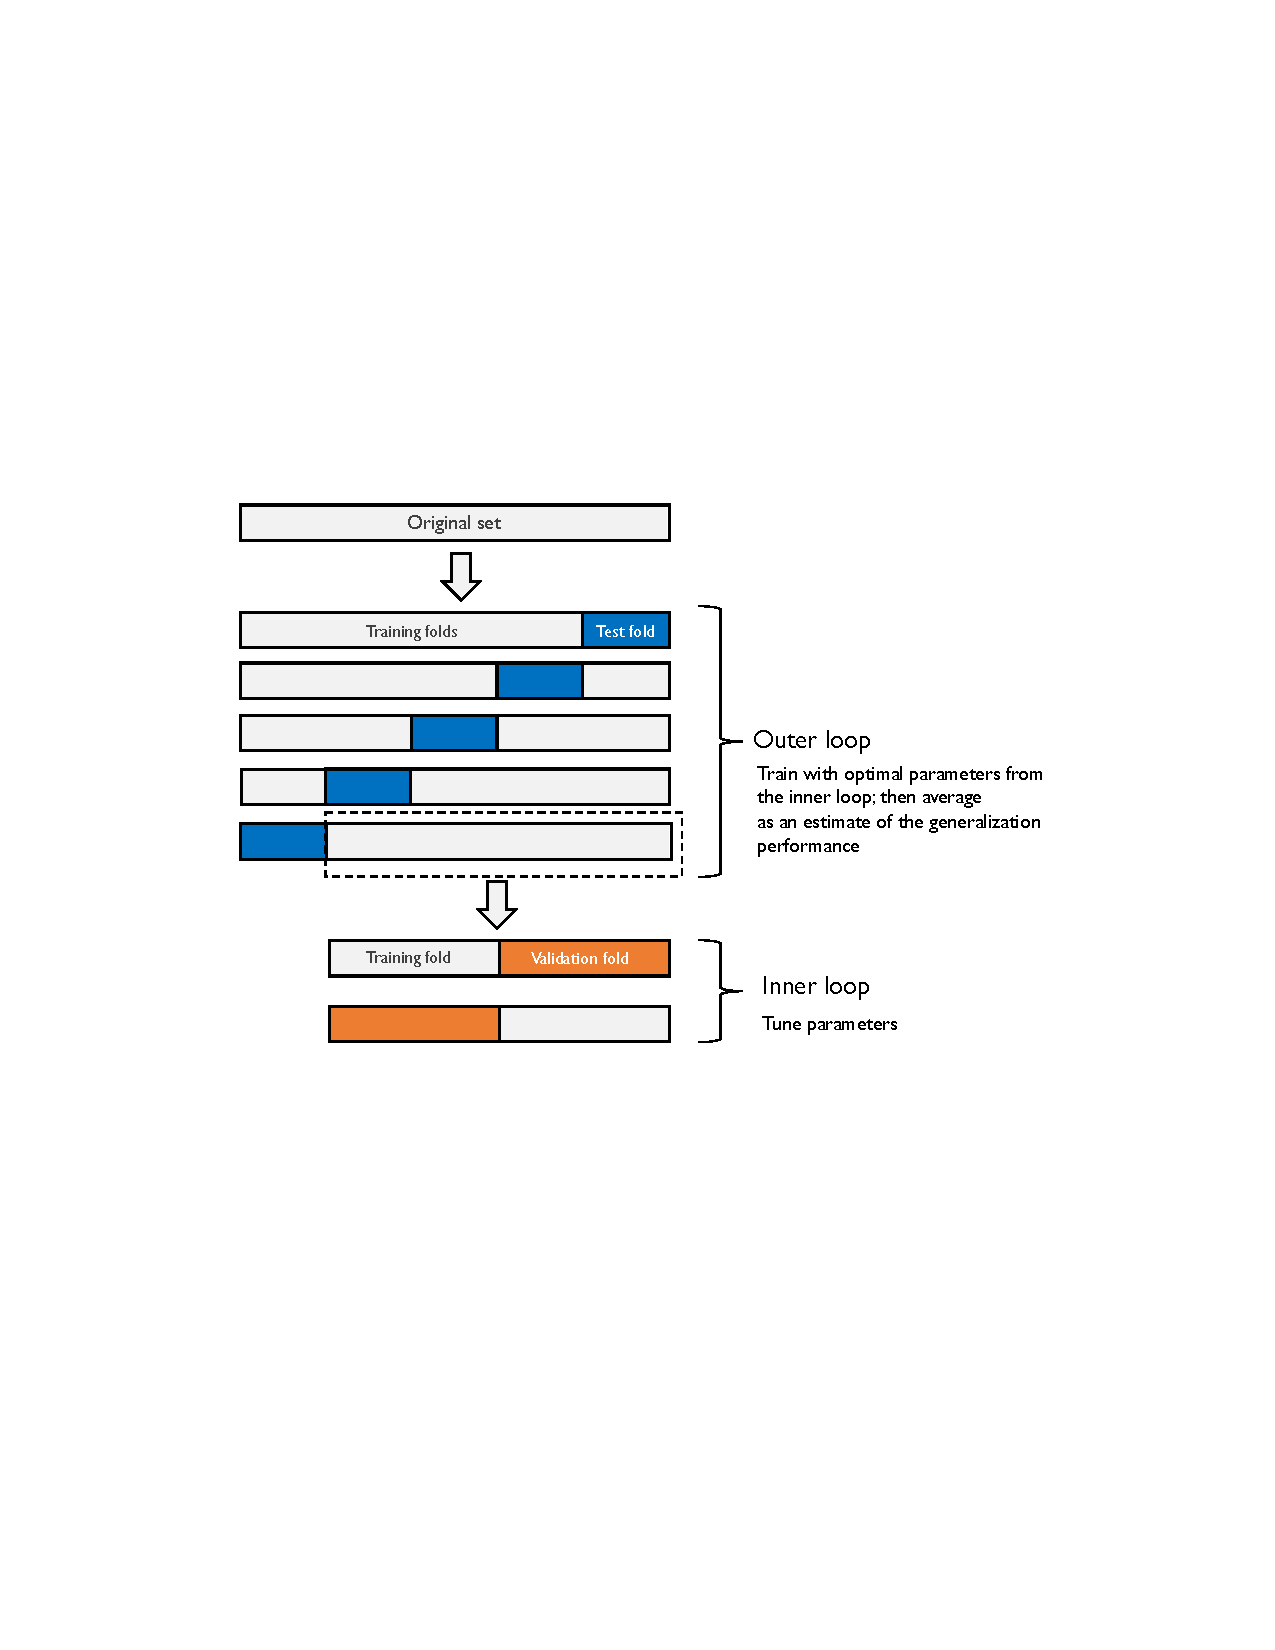
\includegraphics[width=0.8\linewidth]{img/nested_cv.pdf}
    \caption[Esempio \emph{nested cross-validation}.]{Tratto da~\cite{model_evaluation}, esempio di \emph{nested cross-validation}.}
    \label{fig:nested_cv}
\end{figure}

\section{Comuni approcci risolutivi}\label{sec:comuni_approcci_risolutivi}
In questo paragrafo si descrivono brevemente alcuni algoritmi comunemente utilizzati per risolvere i problemi tipici dell'apprendimento automatico categorizzati nel~\Cref{sec:tipi_problemi_ml}.
I modelli \emph{support vector machine}, che sono oggetto specifico del lavoro di tesi, saranno invece descritti in dettaglio nel~\Cref{chap:SVC}.

\subsection{K-Nearest Neighbors}\label{sec:ml:knn}
\emph{K-Nearest Neighbors} (KNN), descritto in dettaglio in~\cite{KNN}, è un algoritmo di apprendimento automatico che può essere utilizzato sia per problemi di classificazione che  per problemi di regressione. 
L'idea alla base del funzionamento è quella di predire un etichetta (continua o discreta) basandosi su una misura di vicinanza per i punti dell'insieme di addestramento. 
Secondo questa caratteristica, così come i modelli \emph{support vector machine} che si vedranno in seguito, anche KNN è un \emph{instance based learner}, ovvero un modello definito da un sottoinsieme di dati di addestramento, utilizzati per fare predizioni su nuovi dati.

Per problemi di classificazione binaria e multi-classe, fissato un intero $K$, KNN individua i $K$ punti dati più vicini a un punto sconosciuto $\Vec{x}_\text{new}$. 
La classe più comune tra questi vicini diventa la classe prevista per il punto $\Vec{x}_\text{new}$. 
In~\Cref{fig:knn_example} si mostra un esempio di classificazione, con $K=3$.
\begin{figure}
    \centering
    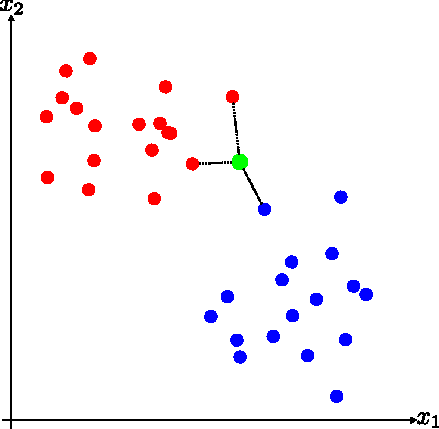
\includegraphics[width=0.7\linewidth]{img/KNN.pdf}
    \caption[Esempio \emph{K-Nearest Neighbors}.]{Esempio di applicazione della regola di classificazione KNN con $K=3$. I colori blu e rosso identificano le due possibili classi. Il punto color verde è il punto per cui predire la classe.
    Il nuovo punto sarà predetto come appartenente alla classe rossa, perché la maggioranza dei dei tre punti a lui più vicini (evidenziati dai segmenti tratteggiati) appartiene a quella classe.}
    \label{fig:knn_example}
\end{figure}

Per problemi di regressione, invece, si calcola la predizione per un punto $\Vec{x}_\text{new}$ come media dei valori dei $K$ punti vicini.

L'utilizzo di un modello KNN richiede di scegliere \emph{a priori} l'iperparametro $K$:
come per altri modelli, risulta necessaria una fase di \emph{model selection} (\Cref{sec:model_selection}) per identificare i migliori iperparametri.
La funzione di misura della distanza tra i dati di addestramento è eventualmente un ulteriore iperparametro modificabile.

KNN è un algoritmo facile da comprendere e implementare, ma ha delle evidenti limitazioni. 
\`E sensibile alla scelta di $K$ ed è particolarmente inadatto per \emph{dataset} di grandi dimensioni, sia a causa dello spazio richiesto per memorizzare il modello appreso (tutti i dati di addestramento), sia (soprattutto) per il costo computazionale, dato che è necessario calcolare la distanza rispetto a ogni elemento per ogni predizione.

Nonostante queste limitazioni, KNN rimane una scelta valida da prendere in considerazione quando si analizzano \emph{dataset} di piccole dimensioni.

\subsection{Alberi di decisione}
Gli alberi di decisione~\cite{decision_tree}, sono modelli che effettuano predizioni basandosi su una struttura dati ad albero, creata durante il processo di addestramento. 
Ogni nodo dell'albero rappresenta una regola, che, valutata su un generico dato $\Vec{x}_\text{new}$, indicherà in quale sotto-albero procedere con la predizione, fino ad arrivare a una foglia che identifica la classe da assegnare. 
In~\Cref{fig:decision_tree} si mostra un esempio di albero di decisione per un problema di classificazione.
Gli alberi di decisione possono anche essere utilizzati per risolvere problemi di regressione.

Il processo di addestramento di un albero decisionale identifica quali sono le regole da utilizzare per raggiungere buone performance di classificazione. 
L'algoritmo di addestramento più noto è CART. 
In questo algoritmo, la bontà di ogni decisione, o in altre parole il criterio con cui creare i nodi interni dell'albero, viene valutata secondo una metrica, tra le più famose si annoverano: \emph{Gini impurity}, \emph{information gain} e \emph{root mean squared error (RMSE)}. 
\begin{figure}
    \centering
    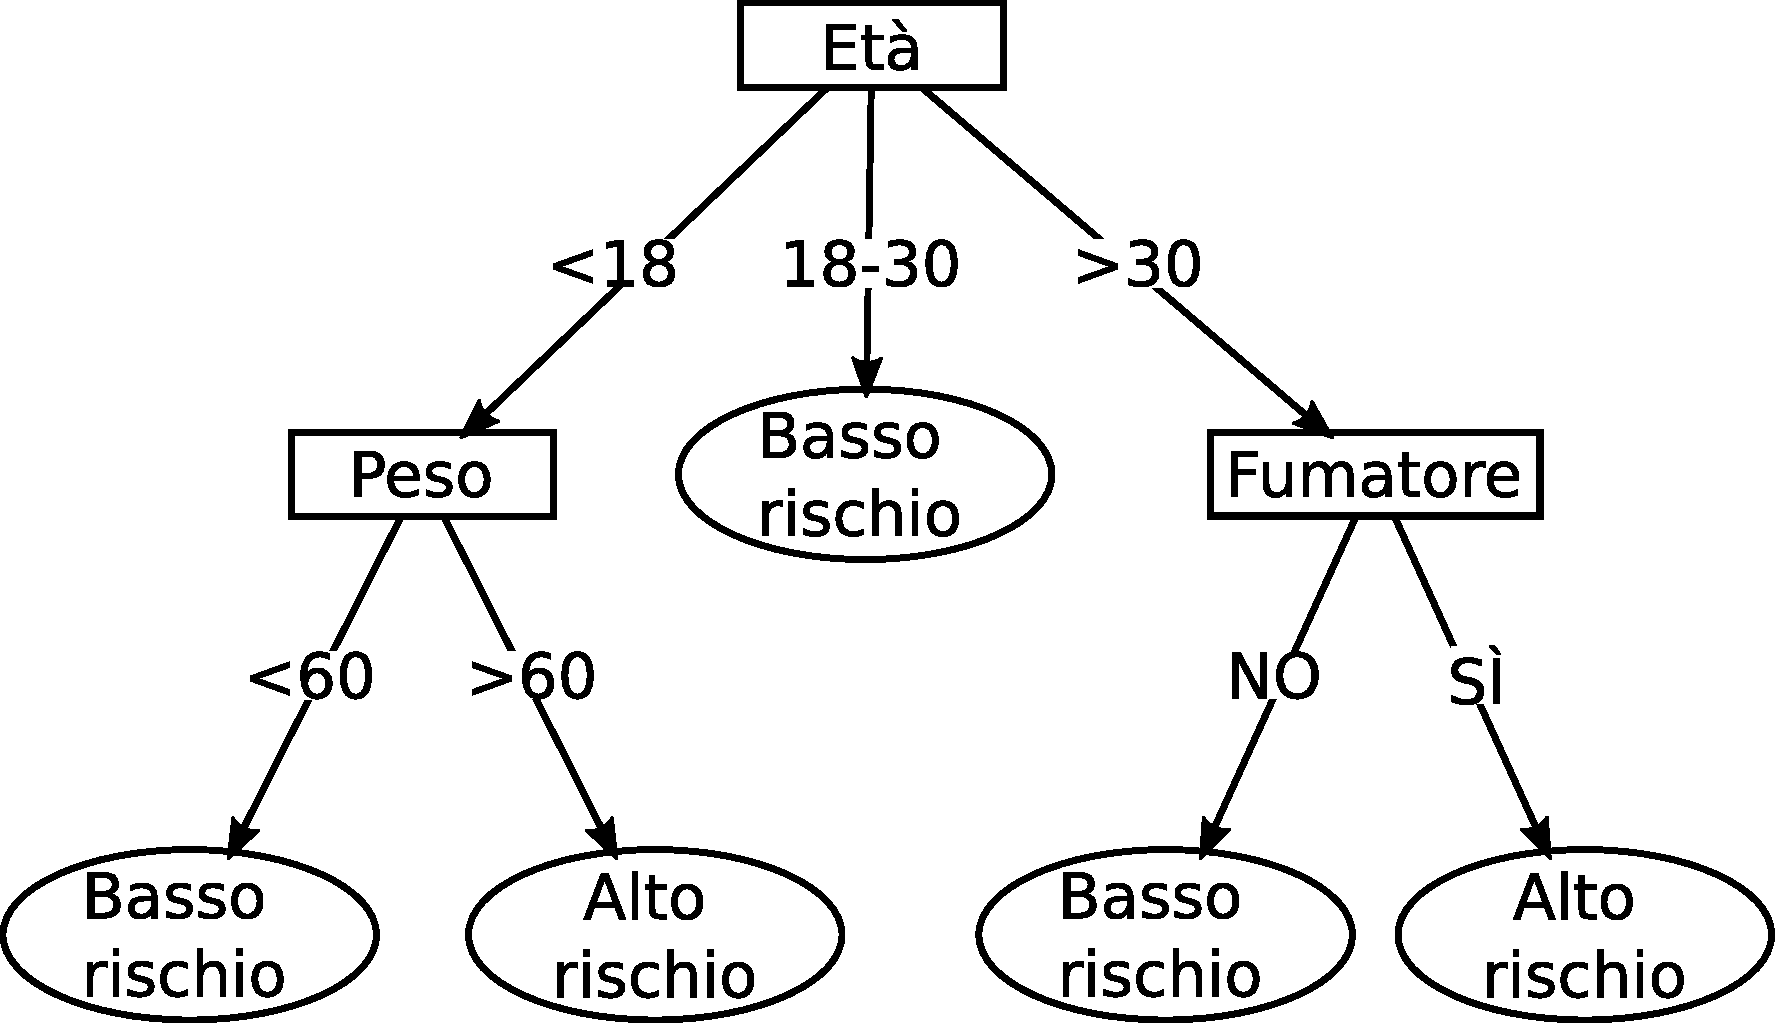
\includegraphics[width=0.7\linewidth]{img/decision_tree.pdf}
    \caption[Esempio albero di decisione.]{Esempio semplificato di un possibile albero di decisione per il rischio di malattia cardiaca. I nodi rettangolari e i corrispettivi archi che collegano ai sotto-alberi identificano delle regole, in questo caso un semplice controllo sull'attributo con il nome del nodo. I nodi foglia ovali identificano il valore della predizione.}
    \label{fig:decision_tree}
\end{figure}
Gli alberi decisionali sono modelli semplici e hanno il pregio di essere modelli \emph{white box}, ovvero sono noti i criteri per cui è eseguita una predizione.
Hanno però la tendenza a essere soggetti al fenomeno dell'\emph{overfitting} (il modello impara troppo fedelmente i dati di addestramento), dato che è sempre possibile ottenere un albero con una foglia per ogni dato di addestramento, e soffrono di \emph{variance error}, dato che anche minimi cambiamenti nell'insieme di addestramento potrebbero avere un'influenza enorme sul modello prodotto.
Queste problematiche saranno meglio discusse nel~\Cref{sec:bias_variance_tradeoff}.
Per queste limitazioni, nella pratica sono molto più utilizzati gli \emph{ensemble} di alberi decisionali, utilizzando tecniche come \emph{bagging}~\cite{bagging_predictors} e \emph{boosting}~\cite{adaboost}.
Un modello \emph{ensemble} è composto da molteplici modelli ``interni'' combinati per ottenere prestazioni migliori; non necessariamente i modelli sono omogenei.
Il tipico esempio di modello \emph{ensemble} è il modello \emph{random forest}, descritto di seguito.

\subsubsection{Random Forest}
Un primo metodo per creare un \emph{ensemble} di alberi decisionali è chiamato \emph{bagging predictors}~\cite{bagging_predictors}, termine che deriva da \emph{\textbf{b}ootstrap} \emph{\textbf{agg}regat\textbf{ing}}.
L'idea alla base del funzionamento è la seguente: il \emph{dataset} di addestramento originale $D$ viene utilizzato per creare $k$ ulteriori \emph{dataset} di dimensioni minori (circa $\frac{2}{3}$ del \emph{dataset} originale) contenenti elementi estratti da $D$ uniformemente a caso con ripetizione.
Su questi $k$ \emph{dataset} si addestrano (singolarmente) altrettanti alberi di decisione, per poi creare un modello unico che aggrega le loro predizioni utilizzando una regola sensata per il problema trattato: per un problema di classificazione, per esempio, si potrebbe utilizzare un voto di maggioranza.

I modelli \emph{random forest}~\cite{random_forest} estendono l'approccio \emph{bagging} introducendo anche la randomizzazione degli attributi. 
Ognuno dei $k$ modelli interni sarà addestrato su un sottoinsieme  di attributi, selezionati casualmente senza ripetizione, una sola volta per l'intero albero oppure a ogni creazione di un nodo interno.
Le predizioni sono poi aggregate come nei \emph{bagging predictors}.
In~\Cref{fig:random_forest} si mostra un esempio schematico di un \emph{ensemble} di alberi.

\begin{figure}
    \centering
    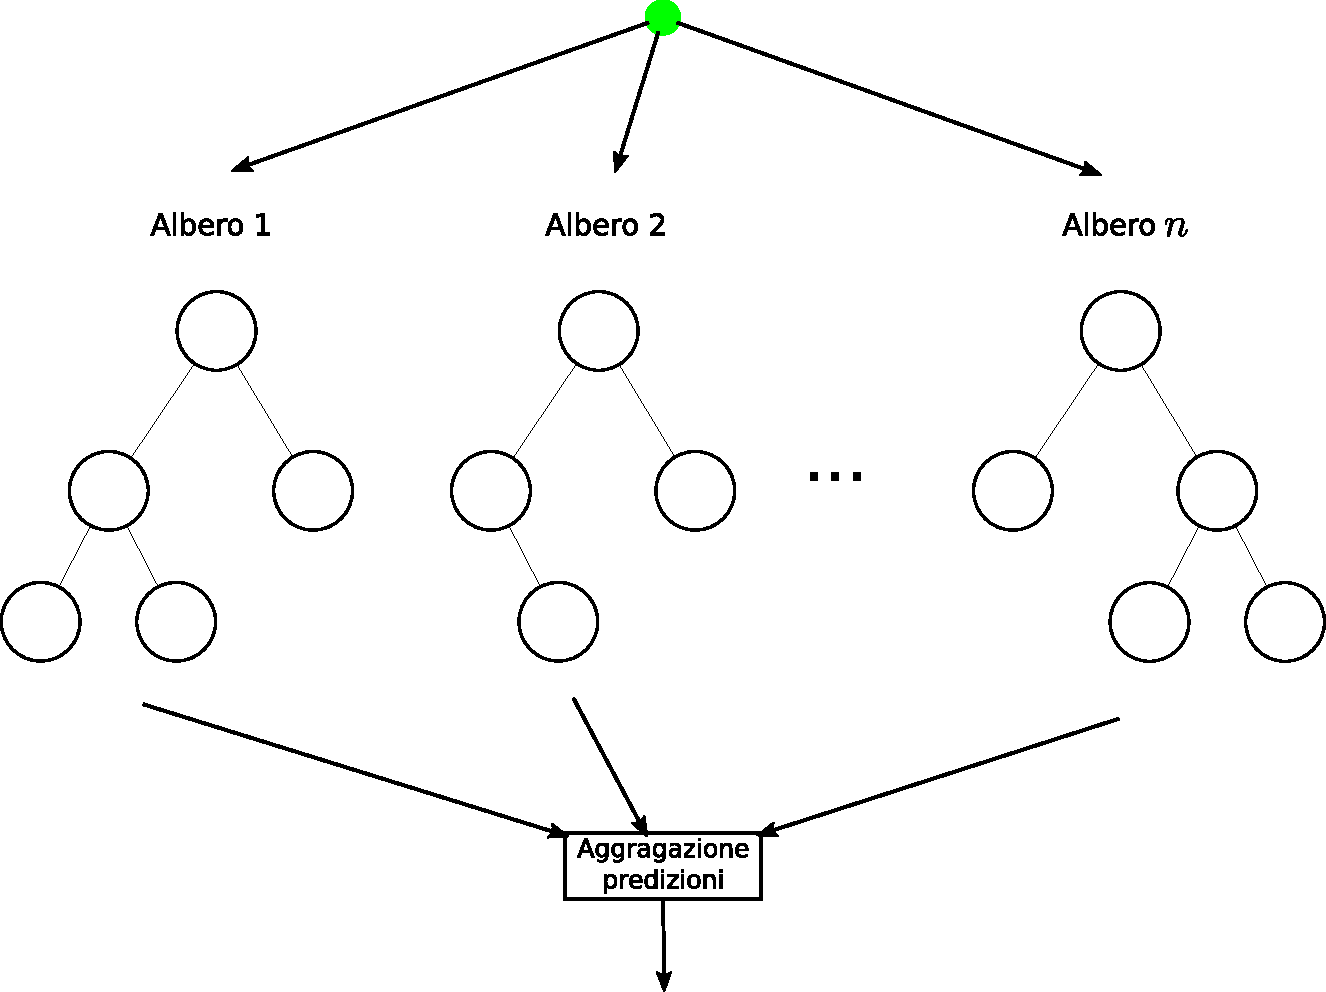
\includegraphics[width=0.7\linewidth]{img/random_forest.pdf}
    \caption[Esempio \emph{random forest}.]{Esempio di \emph{random forest}. Il modello è composto da un insieme di alberi interni, ognuno addestrato su un diverso sottoinsieme di dati e di attributi. Un nuovo esempio da classificare, in questa figura il punto verde, viene classificato da ogni sotto-albero singolarmente, per poi produrre una predizione globale utilizzando una regola di aggregazione delle predizioni interne.}
    \label{fig:random_forest}
\end{figure}

\subsubsection{Boosting}
Un altro approccio per creare \emph{ensamble} di alberi è quello che sfrutta la tecnica chiamata \emph{boosting}, che consiste nel combinare molteplici \emph{weak learner} (in questo caso alberi decisionali molto semplici, anche un solo nodo interno) in modo da ottenere, combinandoli tra loro, uno \emph{strong learner}, ovvero un modello in grado di trattare problemi complessi.
Relativamente agli alberi di decisione gli approcci più famosi sono \emph{AdaBoost}~\cite{adaboost} e \emph{XGboost}~\cite{xgboost}.

%\subsection{Logistic regression}

\subsection{Reti neurali}
Le reti neurali, descritte in dettaglio in~\cite{neural_networks}, sono un tipo di modello di apprendimento automatico ispirato alla struttura del sistema nervoso centrale umano.
Questi modelli imitano il modo in cui i neuroni biologici si scambiano impulsi.
Nella categoria reti neurali rientra una quantità di modelli molto ampia e varia.

Un primo modello di rete neurale è il modello \emph{perceptron} (percettrone)~\cite{1958_perceptron}; viene riportato un esempio in~\Cref{fig:perceptron}.
Un percettrone è un modello di molto semplice composto da un singolo neurone artificiale.
Il neurone riceve in ingresso un vettore $\Vec{x}=[x^{(1)},\dots,x^{(d)}]$ con $\Vec{x} \in \mathbb{R}^d$ ed emette un \emph{output} 
\begin{equation*}
    \hat{y} = \theta\left(\sum_{j=1}^{d}x^{(j)}w^{(j)} +b\right),
\end{equation*} 
dove $w^{(1)},\dots,w^{(d)} \in \mathbb{R}$ sono chiamati pesi, $b \in \mathbb{R}$ è la soglia e $\theta$ è la \emph{funzione di attivazione}, che nel percettrone originale è la \emph{step function} 
\begin{equation*}
    \sigma(x) =
    \begin{cases*}
      1 & se $x>0$, \\
      0 & se $x\leq0$.
    \end{cases*}
\end{equation*}
\begin{figure}
    \centering
    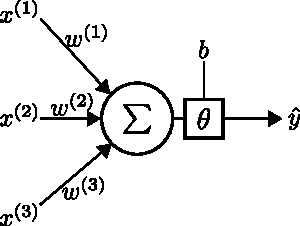
\includegraphics[width=0.3\linewidth]{img/perceptron.pdf}
    \caption[Esempio percettrone.]{Esempio di percettrone. I simboli $x^{(1)},x^{(2)},x^{(3)}$ identificano gli \emph{input}, mentre $\hat{y}$ denota l'\emph{output} del modello. I parametri $w^{(1)},w^{(2)},w^{(3)}$ sono i pesi, mentre $b$ è la soglia opzionale e $\theta$ è la funzione di attivazione.}
    \label{fig:perceptron}
\end{figure}
Il percettrone è un modello semplice, in grado di calcolare funzioni all'interno di una classe piuttosto limitata e quindi non particolarmente espressiva.
Tuttavia, è il modello alla base per la creazione di reti neurali più complesse, come per esempio il percettone multi-strato.

Il percettrone multi-strato è una rete neurale composta da molteplici percettroni collegati tra loro e organizzati in più strati: strato di \emph{input}, uno o più strati nascosti e uno strato di \emph{output}. Si mostra in~\Cref{fig:NN} un esempio di questo tipo di rete. 
A differenza del percettrone, i neuroni delle reti multi-strato utilizzano una funzione di attivazione 
diversa, per esempio la funzione \emph{ReLU} o una funzione sigmoidea.
A seconda del numero di strati nascosti è possibile suddividere questi modelli in \emph{shallow} se con pochi strati o \emph{deep} se con molti strati.
\begin{figure}
    \centering
    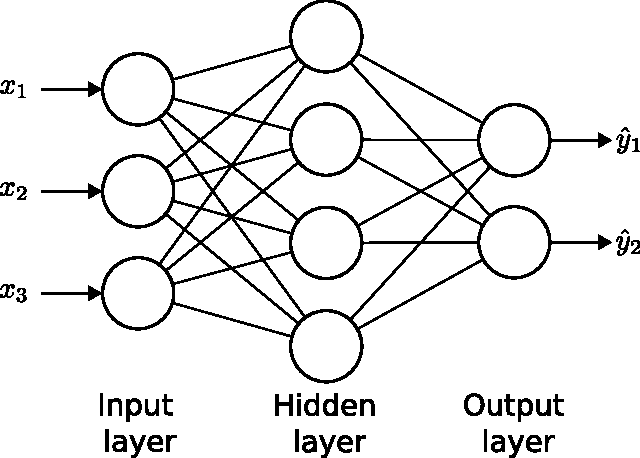
\includegraphics[width=0.5\linewidth]{img/nn.pdf}
    \caption[Esempio percettrone multi-strato.]{Esempio di un semplice percettrone multi-strato con tre neuroni di \emph{input} e due di \emph{output}.}
    \label{fig:NN}
\end{figure}
Le reti neurali descritte fino a ora sono chiamate \emph{feed-forward} perché i dati in fase di predizione fluiscono dallo strato di \emph{input} fino a quello di \emph{output}.
Esistono altre tipologie di reti con strutture più complesse, per esempio le reti ricorrenti, le reti convoluzionali, le reti generative e altre numerose varianti~\cite{aggarwal2018neural}.
In generale, una rete neurale più complessa è composta da molteplici neuroni artificiali, non per forza percettroni; come accennato in precedenza, l'insieme di modelli reti neurali è vasto e variegato.

L'addestramento di una rete neurale \emph{feed-forward} è effettuato con l'algoritmo di retro-propagazione dell'errore~\cite{neural_networks}.
Nella prima fase, \emph{forward-pass}, un insieme di dati passa nella rete fino a produrre le predizioni corrispondenti, per le quali si calcola l'errore. In seguito, percorrendo a ritroso la rete in una fase \emph{backwards-pass}, si aggiustano i pesi e la soglia dei neuroni in modo da ridurre l'errore misurato.
Queste due fasi permettono di calcolare le derivate di una funzione di perdita (per esempio l'accuratezza) rispetto ai pesi e ai bias dei vari neuroni: i valori di queste derivate vengono poi utilizzati per eseguire l'algoritmo del gradiente, col risultato di ottimizzare la funzione di perdita.

In base alla tipologia di rete neurale esistono diversi algoritmi di addestramento, ma in generale si utilizza un metodo del gradiente per ridurre iterativamente l'errore sui dati di addestramento.

L'algoritmo procede iterativamente fino al verificarsi di una condizione di arresto, per esempio il superamento di un numero massimo di istruzioni, o il raggiungimento di un errore di predizione sufficientemente basso.

\section{Bias-variance tradeoff}\label{sec:bias_variance_tradeoff}
Il termine \emph{bias-variance tradeoff}~\cite{elements-of-statistical-learning} si riferisce a una caratterizzazione dell'errore di generalizzazione, ovvero la discrepanza tra i valori effettivi e quelli predetti, relativamente a un insieme di \emph{test} e alle relative implicazioni pratiche.

Il concetto può essere formalizzato come in~\cite{elements-of-statistical-learning}, ma ci si limiterà in questo paragrafo a descriverlo sinteticamente con un esempio.
Si ipotizzi di avere disponibile un \emph{dataset} con le caratteristiche di alcuni pazienti: si pone il compito di costruire un modello per predire se una data persona è a rischio di soffrire di infarto oppure no.
Si consideri ora di costruire un modello molto semplice: un albero di decisione composto da un solo nodo, per cui se l'età del paziente è $>50$ si predice ``rischio alto'', altrimenti si predice ``rischio basso''.
Un modello di questo tipo ha \emph{variance} molto bassa, perché tutto sommato poco sensibile a piccoli cambiamenti nei dati di addestramento. Un paziente con sessanta anni di età ha lo stesso rischio di un paziente con sessanta anni e un giorno di età.
Di contro, questo modello ha \emph{bias} molto alto, perché esegue la predizione solo ed esclusivamente controllando l'età del paziente, evitando di considerare tutte le altre importanti informazioni, facendo di fatto delle assunzioni troppo semplicistiche sulla funzione da approssimare. 
Questo modello non è in grado di approssimare la relazione reale espressa dai dati.
Cambiando approccio, si ipotizzi invece di addestrare un albero di decisione molto profondo, arrivando a generare un nodo foglia per ogni dato di addestramento.
Questo secondo modello avrà \emph{bias} molto basso, perché non farà assunzioni sulla funzione da modellare, anzi ogni possibile attributo sarà valutato per decidere che ramo seguire; allo stesso tempo avrà \emph{variance} molto alta, perché anche una piccola variazione nel dato di \emph{input} risulterà in un percorso nell'albero diverso, ottenendo una predizione potenzialmente molto diversa.
In questo caso, il rischio predetto per un paziente con sessanta anni di età potrebbe essere molto diverso dal rischio predetto per un paziente con sessanta anni e un giorno di età.
Anche questo modello non è in grado di approssimare la relazione reale espressa dai dati in modo soddisfacente.

Un modello con buone capacità di generalizzazione deve esibire basso \emph{bias} e bassa \emph{variance}. Si utilizza il termine \emph{bias-variance tradeoff} (compromesso appunto) perché è molto difficile minimizzare entrambe queste caratteristiche contemporaneamente. In genere, implementare delle tecniche per migliorare il \emph{bias} fa peggiorare la \emph{variance} e viceversa.
Nonostante ciò, è spesso possibile trovare un modello con buone capacità di generalizzazione. 

Questo problema si traduce nella pratica nel problema di \emph{overfitting} e \emph{underfitting}.
Un modello che soffre di \emph{overfitting} (alta \emph{variance}, basso \emph{bias}) è un modello che si è adattato troppo fedelmente ai dati di addestramento, esibendo pessime performance di generalizzazione. 
Un modello che soffre di \emph{underfitting} (alto \emph{bias}, bassa \emph{variance}) è un modello che non è sufficientemente complesso per modellare le relazioni espresse nei dati ed esibisce pessime performance di generalizzazione.
In~\Cref{fig:esempio_underfitting_overfitting} si visualizza un esempio dei vari scenari: \emph{overfitting}, \emph{underfitting} e un esempio di modello con buone capacità di generalizzazione.
\begin{figure}
    \begin{subfigure}[t]{.45\textwidth}
        \centering
        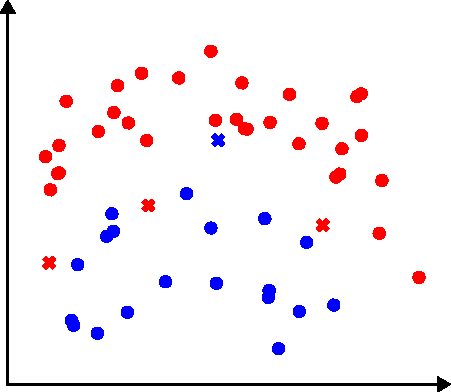
\includegraphics[width=\textwidth]{img/under_over_fitting_1.pdf}
        \caption{Dati di addestramento disponibili. Il colore identifica la classe; i punti scorrettamente etichettati sono indicati con il simbolo x.}
    \end{subfigure}%
    \hfill
    \begin{subfigure}[t]{.45\textwidth}
        \centering
        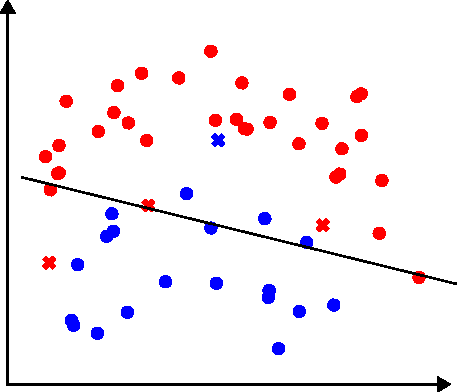
\includegraphics[width=\textwidth]{img/under_over_fitting_2.pdf}
        \caption{Esempio di come un modello lineare potrebbe esibire \emph{underfitting}.}
    \end{subfigure}%
\vskip\baselineskip
    \begin{subfigure}[t]{.45\textwidth}
        \centering
        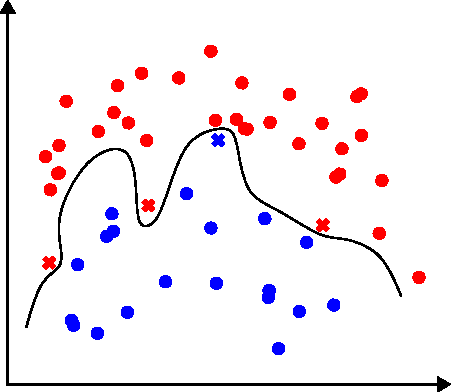
\includegraphics[width=\textwidth]{img/under_over_fitting_3.pdf}
        \caption{Esempio di come un modello non lineare potrebbe esibire \emph{overfitting}.}
    \end{subfigure}%
    \hfill
    \begin{subfigure}[t]{.45\textwidth}
        \centering
        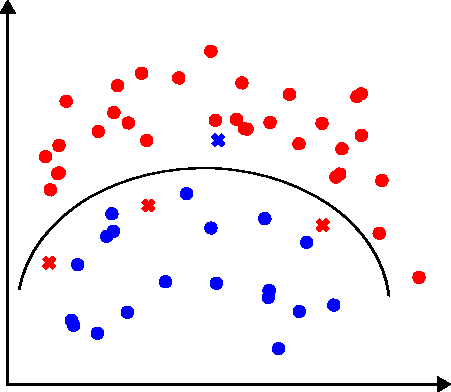
\includegraphics[width=\textwidth]{img/under_over_fitting_4.pdf}
        \caption{Esempio di una possibile superficie di separazione con buone capacità di generalizzazione.}
    \end{subfigure}%
\caption[Esempio di \emph{underfitting} e \emph{overfitting}.]{Esempio di \emph{underfitting} e \emph{overfitting} su un \emph{dataset} per un problema di classificazione binaria.}
\label{fig:esempio_underfitting_overfitting}
\end{figure}
    \chapter{Support Vector Machine}\label{chap:SVC}
In questo capitolo si descrive genericamente la famiglia dei modelli \emph{support vector machine} (SVM) e in dettaglio la formulazione del modello per risolvere problemi di classificazione (\emph{support vector classifier}, o SVC). 
Nel~\Cref{sec:kernel_methods} si fornisce una breve introduzione ai metodi \emph{kernel} e alla famiglia dei modelli SVM. 
Nel~\Cref{sec:hard_margin_classifier} si descrive la formulazione \emph{hard margin} per problemi di classificazione, che non ammette dati erroneamente etichettati.
Nel~\Cref{sec:soft_margin_classifier} si descrive la formulazione \emph{soft margin} per problemi di classificazione, che ammette la presenza di dati erroneamente etichettati.
Nel~\Cref{sec:kernel_trick} si descrive l'utilizzo del metodo \emph{kernel} per i modelli SVC.
Per concludere, nel~\Cref{sec:svc_limiti} si descrivono in generale le principali limitazioni dei modelli SVM.

\section{Metodi kernel}\label{sec:kernel_methods}
\`E possibile suddividere i modelli di apprendimento automatico in due categorie: modelli lineari e modelli non lineari. 
I modelli lineari vengono utilizzati nei casi in cui si assume che la relazione tra i dati di addestramento $\Vec{x}$ e le etichette $y$ possa essere approssimata in modo accettabile da una funzione lineare $f(\Vec{x}) = \Vec{w}\cdot\Vec{x} + b$, mentre i modelli non lineari sono in grado di approssimare relazioni più complesse.
%I modelli non lineari vengono utilizzati nei casi in cui questa assunzione non si dimostra vera, e per cui serve definire una funzione più complessa per approssimare la relazione.
In genere, produrre un modello lineare è relativamente facile, ma molti scenari reali esprimono relazioni non lineari. 
Adottare un modello lineare in questi casi porterebbe ad insufficienti capacità di generalizzazione, dovute alla troppa semplicità del modello (\emph{underfitting}). 
\`E quindi necessario sviluppare algoritmi per produrre modelli in grado di esprimere relazioni non lineari, ma utilizzare un modello più complesso potrebbe comunque portare ad insufficienti capacità di generalizzazione. 
Questo problema si potrebbe verificare nel caso in cui il modello si adatti troppo fedelmente ai dati di addestramento (\emph{overfitting}).
Questa problematica è descritta nel~\Cref{sec:bias_variance_tradeoff}; mentre in~\Cref{fig:esempio_underfitting_overfitting} si mostrano esempi di \emph{underfitting} o \emph{overfitting}.

Si vorrebbe quindi un modello sufficientemente complesso per approssimare la relazione espressa dai dati, ma allo stesso tempo non troppo complesso da soffrire di \emph{overfitting}; si vorrebbe la semplicità di un modello lineare con le capacità di modellazione di un modello non lineare. 
% TODO: potrebbe benissimo andare nel capitolo 1
\begin{figure}
    \begin{subfigure}[t]{.45\textwidth}
        \centering
        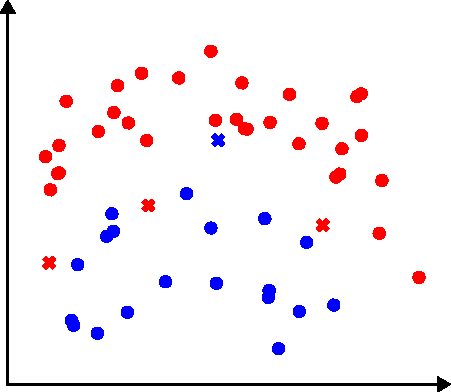
\includegraphics[width=\textwidth]{img/under_over_fitting_1.pdf}
        \caption{Il colore identifica la classe; i punti scorrettamente etichettati sono indicati con il simbolo x.}
    \end{subfigure}%
    \hfill
    \begin{subfigure}[t]{.45\textwidth}
        \centering
        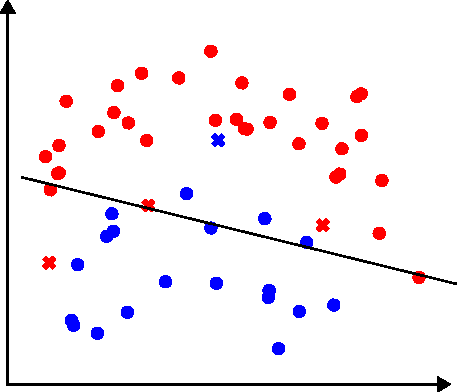
\includegraphics[width=\textwidth]{img/under_over_fitting_2.pdf}
        \caption{Esempio di come un modello lineare potrebbe esibire \emph{underfitting}.}
    \end{subfigure}%
\vskip\baselineskip
    \begin{subfigure}[t]{.45\textwidth}
        \centering
        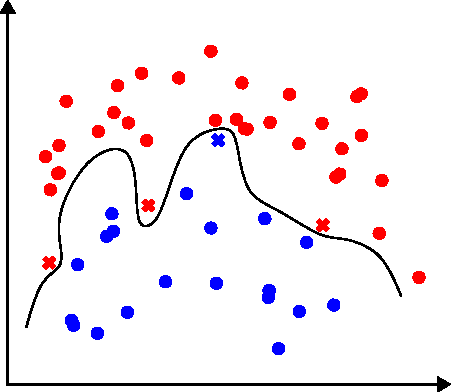
\includegraphics[width=\textwidth]{img/under_over_fitting_3.pdf}
        \caption{Esempio di come un modello non lineare potrebbe esibire \emph{overfitting}.}
    \end{subfigure}%
    \hfill
    \begin{subfigure}[t]{.45\textwidth}
        \centering
        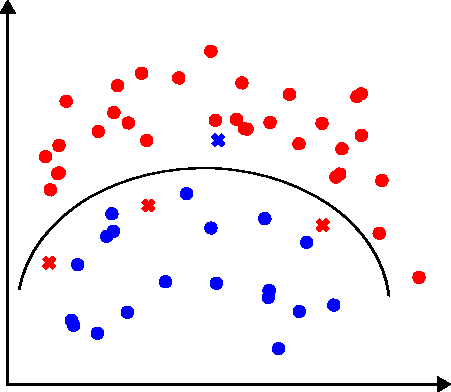
\includegraphics[width=\textwidth]{img/under_over_fitting_4.pdf}
        \caption{Esempio di una possibile superficie di separazione con buone capacità di generalizzazione.}
    \end{subfigure}%
\caption{Esempio di \emph{underfitting} e \emph{overfitting} su un dataset per un problema di classificazione binaria.}
\label{fig:esempio_underfitting_overfitting}
\end{figure}

I \emph{metodi kernel}~\cite{2007_kernel_methods} sono una famiglia di approcci per risolvere vari problemi tipici dell'apprendimento automatico. La particolarità sta nel fatto che non si tratta di metodi creati \emph{ad hoc}, ma di estensioni di algoritmi lineari già noti, potenziati per poter esprimere relazioni più complesse.
L'idea alla base dei metodi \emph{kernel} è di mappare i dati dallo spazio originale $\mathcal{X}$ ad un nuovo spazio $\mathcal{H}$, chiamato \emph{spazio delle feature}, di dimensionalità maggiore rispetto ad $\mathcal{X}$, potenzialmente infinita, utilizzando la trasformazione non lineare $\Phi: \mathcal{X} \rightarrow \mathcal{H}$.
Nello spazio delle \emph{feature} i dati diventano linearmente separabili, ed è quindi possibile utilizzare un modello lineare espresso esclusivamente in termini di prodotto scalare tra elementi in $\mathcal{H}$, ma che esprime una relazione non lineare in $\mathcal{X}$.

Questo procedimento è però costoso dal punto di vista computazionale: va calcolata $\Phi$ per ogni punto e poi va calcolato il prodotto interno tra tutte le coppie di elementi.
I metodi \emph{kernel} evitano di utilizzare esplicitamente la funzione $\Phi$, utilizzando invece una funzione
%Nei metodi \emph{kernel} lo spazio delle \emph{feature} è un \emph{reproducing kernel Hilbert space} (RKHS) \cite{}: questo consente di esprimere il prodotto scalare tra elementi appartenenti ad $\mathcal{H}$ con una funzione espressa in termini di prodotto scalare tra elementi di $\mathcal{X}$. Esiste quindi la funzione 
\begin{equation*}
    K: \mathcal{X} \times \mathcal{X} \rightarrow \mathbb{R} 
\end{equation*}
per cui per ogni $\Vec{x}, \Vec{z} \in \mathcal{X}$ vale
\begin{equation*}
    K(\Vec{x}, \Vec{z}) = \Phi(\Vec{x}) \cdot \Phi(\Vec{z}).
\end{equation*}
Questa funzione $K$ è chiamata \emph{funzione kernel}.
Un metodo \emph{kernel} è un algoritmo di addestramento che riesce a sfruttare una funzione \emph{kernel} nelle fasi di addestramento e predizione, rendendo in questo modo non necessario l'utilizzo di $\Phi$, perché il prodotto scalare delle immagini $\Phi(\Vec{x}) \cdot \Phi(\Vec{z})$ è funzione del prodotto scalare tra $\Vec{x}, \Vec{z}$ nello spazio originale.
Questo calcolo è possibile perché $\mathcal{H}$ è un \emph{reproducing kernel Hilbert space} (RKHS)~\cite{RKHS}.

Con un metodo \emph{kernel} si cerca di sfruttare la semplicità di un modello lineare nello spazio delle \emph{feature} ma in grado di modellare relazioni complesse nello spazio originale.
Il~\Cref{sec:kernel_trick} riporta una spiegazione più approfondita dell'applicazione del metodo \emph{kernel} ai modelli SVC.

Tra i metodi \emph{kernel} più noti possiamo citare \emph{kernel principal component analysis}~\cite{kernel_PCA} o \emph{kernel perceptron}~\cite{kernel_perceptron}, ma l'approccio forse più importante è quello relativo alla famiglia delle \emph{support vector machine}, che include varianti per risolvere sia problemi di classificazione che di regressione.
Introdotti inizialmente per problemi di classificazione, i modelli SVC estendono il concetto di \emph{maximal margin classifier}. 
L'addestramento di un modello SVC ha come obiettivo quello di trovare un iperpiano che separa i punti appartenenti a due classi diverse con il massimo margine di separazione ottenibile. 
Questo approccio era inizialmente limitato a problemi lineari senza ammissione di dati erroneamente etichettati. 
Nei primi anni novanta, con l'introduzione del metodo \emph{kernel}~\cite{1992_hardmargin_svm} prima e con l'introduzione della formulazione \emph{soft margin}~\cite{1995_svm} poi, i modelli SVC divennero delle buone opzioni per risolvere problemi di classificazione non lineari e con dati erroneamente etichettati, riscuotendo un buon successo e ottenendo in alcuni casi \emph{performance} comparabili e spesso superiori ad altri modelli avanzati. 

Si trovano in letteratura diversi approcci che modificano la formulazione SVM originale, come per esempio \emph{$\nu$-svm}\cite{2000_nu_svm} o  \emph{p-svm}\cite{2001_p_svm}.
In questa tesi si presterà particolare attenzione alla formulazione originale per risolvere problemi di classificazione, dato che è la formulazione di partenza considerata per l'approccio proposto nel~\Cref{sec:our_budgeted_svm}.

Le formulazioni dei modelli SVC esposte nei prossimi paragrafi sono estratte in gran parte da~\cite{1995_svm,svm_tutorial,elements-of-statistical-learning}.

\section{Classificazione \emph{hard margin}}\label{sec:hard_margin_classifier}
Si ipotizza di avere un insieme di dati $\mathcal{X} = \{\Vec{x}_i, i=1,\dots,m\}$ contenente $m$ vettori $d$-dimensionali, $\Vec{x}_i \in \mathbb{R}^d$. 
Ogni $\Vec{x}_i$ ha associata un'etichetta $y_i \in \{-1, +1\}$: si considerano quindi problemi di classificazione binaria.
%
L'insieme $\mathcal{X}$ è linearmente separabile se esistono un vettore $\Vec{w} \in \mathbb{R}^d$ e uno scalare $b \in \mathbb{R}$ (chiamato \emph{bias}) che identificano un iperpiano $\Vec{w}\cdot \Vec{x} +b=0$ in grado di separare perfettamente le due classi di dati.
\begin{figure}
    \centering
    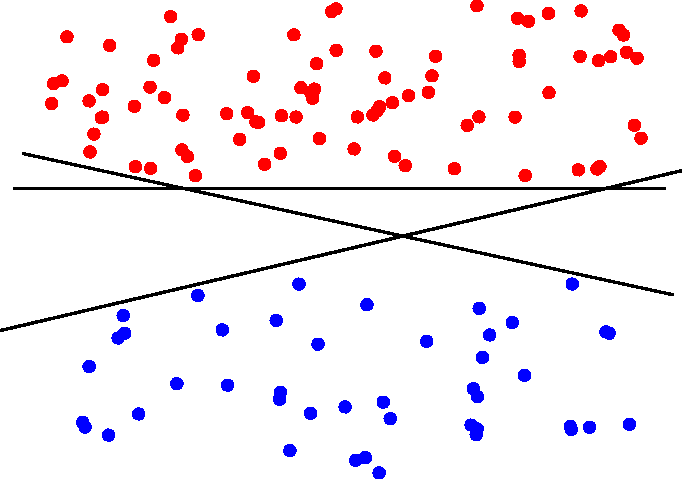
\includegraphics[width=0.5\linewidth]{img/dati_linearmente_separabili.pdf}
    \caption{Esempio di dati per un problema di classificazione binaria in cui le classi (identificate dai due colori rosso e blu) sono linearmente separabili. Sono illustrate alcune delle possibili rette in grado di separare correttamente tutti gli esempi della stessa classe. }
    \label{fig:dati_linearmente_separabili}
\end{figure}
Con $\Vec{w}$ e $b$ noti, si definisce il classificatore 
\begin{equation*}
    h(\Vec{x}) = \sign(\Vec{w}\cdot \Vec{x} +b).
\end{equation*} 
Per insiemi di dati linearmente separabili esistono infiniti iperpiani che li separano; l'interesse è di trovare un iperpiano con cui eseguire predizioni accurate su nuovi dati. 
Si riporta in~\Cref{fig:dati_linearmente_separabili} un esempio di insieme di dati con alcuni possibili superfici di separazione. 
Per costruire un buon classificatore, in grado di generalizzare su dati mai visti nella procedura di addestramento, si vorrebbe identificare l'iperpiano che massimizza il margine di separazione tra le due classi, ovvero l'iperpiano che massimizza la distanza tra l'iperpiano stesso e i punti più vicini di ogni classe.
La superficie di separazione deve essere equidistante rispetto agli esempi più vicini di ogni classe.

Per configurare un problema trattabile è necessario quantificare il margine.
Sia $d$ la distanza tra la superficie di separazione e il punto più vicino etichettato come positivo. 
Dato che si vorrebbero separare al meglio le due classi, la superficie di separazione dovrà trovarsi alla stessa distanza anche rispetto al punto più vicino etichettato come negativo.
In~\Cref{fig:optimal_separation_margin} si può vedere un esempio per un insieme di dati in due dimensioni.
Il margine è quindi $M=2d$, ma è possibile trasformarlo in una forma più conveniente.
Si definiscono a tale scopo i vincoli 
\begin{equation*}\label{eq:svc:hardmargin:margin_1}
    \Vec{w}\Vec{x}_i + b \geq 1 \quad \text{se} \quad y_i = +1 \quad  i=1,\dots,m,
\end{equation*}
\begin{equation*}
    \Vec{w}\Vec{x}_i + b \leq -1 \quad \text{se} \quad y_i = -1 \quad i=1,\dots,m,
\end{equation*}
che forzano la superficie di separazione ad essere equidistante dagli iperpiani su cui giacciono i punti più vicini di ogni classe.
% Dividendo entrambi i lati delle disequazioni per $M$
% \begin{equation*}
% \frac{1}{M}\Vec{w}\Vec{x}_i + \frac{1}{M}b \geq 1,
% \end{equation*}
% \begin{equation*}
% \frac{1}{M}\Vec{w}\Vec{x}_i + \frac{1}{M}b \leq -1,
% \end{equation*}
% otteniamo come iperpiano di classificazione $\frac{1}{M}\Vec{w}\Vec{x}_i + \frac{1}{M}b = 0,$ che è equivalente a $\Vec{w}\Vec{x}_i + b = 0$. Il parametro $M$ è quindi in genere fissato ad $1$.
Dato che $y_i\in\{-1,1\}$, i vincoli precedenti possono essere combinati in
\begin{equation*}
    y_i(\Vec{w}\Vec{x}_i + b) \geq 1 \quad i=1, ..., m.
\end{equation*}
Considerando i punti per cui il vincolo precedente è un'uguaglianza: i punti positivi saranno sull'iperpiano $H1: \vec{w}\cdot \vec{x} + b=+1$, con vettore normale $\vec{w}$ e distanza dall'origine $|1-b|/\norm{\vec{w}}$, mentre i punti negativi saranno sull'iperpiano $H2: \vec{w}\cdot \vec{x} + b=-1$, con vettore normale $\vec{w}$ e distanza dall'origine $|-1-b|/\norm{\vec{w}}$. Si può dimostrare che la distanza $2d$ è equivalente a $2/\norm{\vec{w}}$~\cite{svm_tutorial}.

L'iperpiano ottimo $H0: \Vec{w}^*\Vec{x} + b^* = 0$ è l'iperpiano che separa linearmente $\mathcal{X}$ massimizzando il margine di separazione; il simbolo $*$ indica il valore ottimo di una variabile.

I punti $\Vec{x}_i$ per cui $\Vec{w}^*\Vec{x}_i + b^* = \pm 1$ sono chiamati \emph{vettori di supporto}.
\begin{figure}
    \centering
    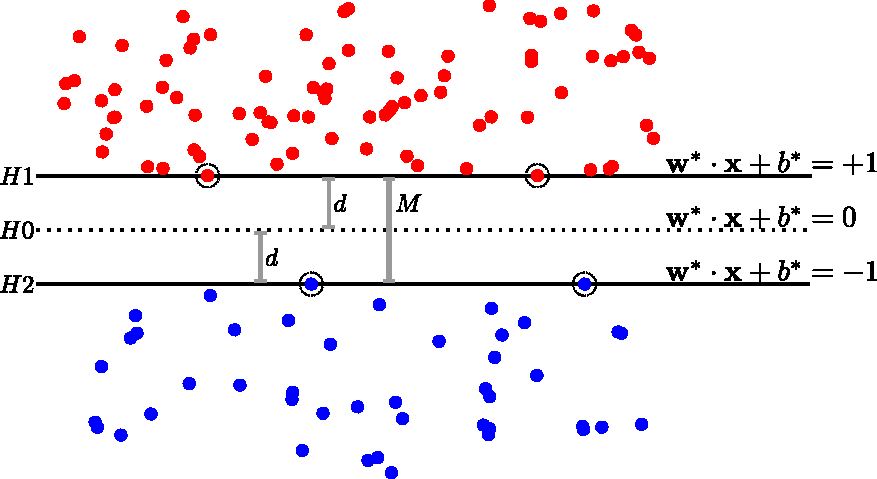
\includegraphics[width=0.7\linewidth]{img/margine_separazione.pdf}
    \caption{Esempio di superficie di separazione con margine massimale per gli stessi dati utilizzati in~\Cref{fig:dati_linearmente_separabili}. I punti cerchiati sono vettori di supporto. $H0$ è la superficie di separazione, mentre $H1$ e $H2$ sono le superfici su cui giacciono i vettori di supporto. Il margine è $M=2d$.}
    \label{fig:optimal_separation_margin}
\end{figure}
%
Massimizzare il margine $2/\norm{\vec{w}}$ equivale a minimizzare $\norm{\Vec{w}}$. 
Trovare la superficie di separazione con margine massimale equivale quindi a risolvere il problema di ottimizzazione
\begin{equation}
\label{eq:svc:hardmargin:primal}
\begin{aligned}
& \min_{\Vec{w},b} && \norm{\Vec{w}} \\
& \textrm{s.t.} && y_i(\Vec{w}\cdot \Vec{x}_i + b) \geq 1, && i=1,\dots,m. \\
\end{aligned}
\end{equation}
Questo problema viene tradizionalmente risolto considerando una formulazione duale, che consente l'impiego del metodo \emph{kernel} più facilmente rispetto alla formulazione primale.

\subsection{Formulazione duale}\label{subsec:hard_margin_dual}
Si riscrive la funzione obiettivo del problema primale in~\Cref{eq:svc:hardmargin:primal} in una forma più conveniente e si esprimono i vincoli in forma normale, ottenendo il problema
\begin{equation}\label{eq:svc:hardmargin:primal_convenient}
\begin{aligned}
& \min_{\Vec{w},b}    && \frac{1}{2}\norm{\Vec{w}}^2 \\
& \textrm{s.t.} && y_i(\Vec{w}\cdot \Vec{x}_i + b) - 1 \geq 0, && i=1,\dots,m, \\
\end{aligned}
\end{equation}
con funzione obiettivo quadratica e vincoli lineari.
%
Applicando il metodo dei moltiplicatori di Lagrange~\cite{optimization_book} si ottiene la funzione lagrangiana
\begin{equation}
\label{eq:svc:hardmargin:lagrangian}
\begin{split}
L_P(\Vec{w},b, \vec{\alpha})  & = \frac{1}{2}\norm{\Vec{w}}^2 - \sum_{i=1}^{m} \alpha_i (y_i(\Vec{w}\cdot \Vec{x}_i +b) -1) =\\
        & = \frac{1}{2}\Vec{w} \cdot \Vec{w} - \sum_{i=1}^{m} \alpha_i y_i(\Vec{w}\cdot \Vec{x}_i +b) -  \sum_{i=1}^{m} - \alpha_i = \\
        & = \frac{1}{2}\Vec{w}\cdot\Vec{w} - \sum_{i=1}^{m} \alpha_i y_i \Vec{w}\cdot \Vec{x}_i - b \sum_{i=1}^{m} \alpha_i y_i + \sum_{i=1}^{m} \alpha_i,
\end{split}
\end{equation}
da minimizzare rispetto a $\Vec{w},b$ e da massimizzare rispetto ad $\Vec{\alpha}$ 
\begin{equation}
\label{eq:svc:hardmargin:max_min}
\begin{aligned}
& \max_{\vec{\alpha}} \min_{\Vec{w}, b} && L_P(\Vec{w},b, \Vec{\alpha}) \\
& \textrm{s.t.} && \alpha_i \geq 0, && i=1,..., m.\\
\end{aligned}
\end{equation}
%
%
Una soluzione ottima per il problema~\Cref{eq:svc:hardmargin:max_min} deve soddisfare le condizioni di Karush-Kuhn-Tucker (KKT)~\cite{svm_tutorial,optimization_book}:
\begin{align}
    \label{eq:svc:hardmargin:kkt1}
    \pd{L_P(\Vec{w},b,\vec{\alpha})}{\Vec{w}} = \Vec{0}, \\[2mm]
    \label{eq:svc:hardmargin:kkt2}
    \pd{L_P(\Vec{w},b,\vec{\alpha})}{b} = 0, 
\end{align}
\begin{align}
    \label{eq:svc:hardmargin:kkt3}
    y_i(\Vec{x}_i\cdot\Vec{w}+b)-1 \geq 0, && i=1,\dots,m,  \\[2mm]
    \label{eq:svc:hardmargin:kkt4}
    \alpha_i \geq 0, && i=1,\dots,m,  \\[2mm]
    \label{eq:svc:hardmargin:kkt5}
    \alpha_i^*(y_i(\Vec{x}_i\cdot\Vec{w}^*+b^*)-1) = 0,  && i=1,\dots,m.
\end{align}
%Il problema~\ref{eq:svc:hardmargin:max_min} è quadratico convesso **fidatevi**.
%
Le condizioni nelle~\Cref{eq:svc:hardmargin:kkt1,eq:svc:hardmargin:kkt2}, ovvero
\begin{align*}
    \pd{L_P}{\Vec{w}} &= \Vec{w} - \sum_{i=1}^{m}\alpha_iy_i\Vec{x}_i = \Vec{0},\\
    \pd{L_P}{b} &=  \sum_{i=1}^{m}\alpha_iy_i =0,
\end{align*}
si riducono a
\begin{equation}
\label{eq:svc_sub1}
\Vec{w} = \sum_{i=1}^{m}\alpha_iy_i\Vec{x}_i,
\end{equation}
\begin{equation}
\label{eq:svc_sub2}
\sum_{i=1}^{m}\alpha_iy_i = 0.
\end{equation}
% representer theorem [Kimeldorf and Wahba,1971] tells us that the optimal solution w∗ of the primal problem can be represented as a linear combination
Sostituendo le~\Cref{eq:svc_sub1,eq:svc_sub2} nella funzione~(\ref{eq:svc:hardmargin:lagrangian}) si ottiene la funzione obiettivo duale
\begin{equation}
\label{eq:svc:hardmargin:dual_obj_fn}
\begin{split}
L_D(\vec{\alpha})  & = \frac{1}{2}\Vec{w}\cdot\Vec{w} - \sum_{i=1}^{m} \alpha_i y_i \Vec{w}\cdot \Vec{x}_i - b \sum_{i=1}^{m} \alpha_i y_i + \sum_{i=1}^{m} \alpha_i =\\
 &= \frac{1}{2}\sum_{i=1}^{m}\alpha_iy_i\Vec{x}_i \cdot \sum_{i=1}^{m}\alpha_iy_i\Vec{x}_i - \sum_{i=1}^{m} \alpha_i y_i \Vec{x}_i \sum_{j=1}^{m}\alpha_jy_j\Vec{x}_j + \sum_{i=1}^{m} \alpha_i =\\
 &= \frac{1}{2}\sum_{i=1}^{m}\sum_{j=1}^{m}\alpha_i\alpha_jy_iy_j\Vec{x}_i\cdot\Vec{x}_j - 
 \sum_{i=1}^{m}\sum_{j=1}^{m}\alpha_i\alpha_jy_iy_j\Vec{x}_i\cdot\Vec{x}_j + \sum_{i=1}^{m} \alpha_i =\\
 &= -\frac{1}{2}\sum_{i=1}^{m}\sum_{j=1}^{m}\alpha_i\alpha_jy_iy_j\Vec{x}_i\cdot\Vec{x}_j + \sum_{i=1}^{m} \alpha_i,
\end{split}  
\end{equation}
espressa esclusivamente in funzione di $\Vec{\alpha}$.
Aggiungendo i rimanenti vincoli di non negatività di $\vec{\alpha}$ si ottiene il problema duale
\begin{equation}\label{eq:svc:hardmargin:wolfe_dual}
\begin{aligned}
& \max_{\vec\alpha}     && \sum_{i=1}^{m}\alpha_i - \frac{1}{2}\sum_{i=1}^{m}\sum_{j=1}^{m}\alpha_i\alpha_jy_iy_j\Vec{x}_i\cdot\Vec{x}_j\\
& \textrm{s.t.}     && \sum_{i=1}^{m} \alpha_iy_i = 0, \\
&                   && \alpha_i \geq 0 && i=1,\dots,m. \\
\end{aligned}
\end{equation}
%
Una volta risolto il problema duale~\Cref{eq:svc:hardmargin:wolfe_dual} all'ottimo, si otterranno i valori ottimali per i moltiplicatori lagrangiani $\alpha_1^*, ..., \alpha_m^*$.
Ricordando che $\Vec{w} = \sum_{i=1}^{m}\alpha_iy_i\Vec{x}_i$, è possibile calcolare l'ottimo 
\begin{equation}\label{eq:representer_w} %??
\Vec{w}^* = \sum_{i=1}^{m}\alpha_i^*y_i\Vec{x}_i.
\end{equation}
Il vettore $\Vec{w}^*$ è definito dai i dati di addestramento $\Vec{x}_i, y_i$ con un corrispettivo moltiplicatore lagrangiano $\alpha_i > 0$: i vettori di supporto. 
Questi punti definiscono il modello: se si rimuovessero tutti i punti che non sono vettori di supporto e si ripetesse l'addestramento, si otterrebbe lo stesso risultato.
Tutti gli $\Vec{x}_i$ associati ad un moltiplicatore lagrangiano ottimo nullo $\alpha_i=0$ non influiscono sulla superficie di separazione.
Per comodità, si definisce l'insieme
\begin{equation*}
    S = \{i \in \{1,\dots,m\} :\alpha_i >0\},   
\end{equation*}
che contiene tutti gli indici corrispondenti a vettori di supporto.

I modelli SVC si possono inserire nella categoria degli \emph{instance based learner}, dato che eseguono predizioni utilizzando un sottoinsieme dei dati di addestramento.

Per costruire il classificatore $h(\Vec{x}) = \sign(\Vec{w}\cdot \Vec{x} +b)$ rimane ancora da calcolare $b$.  Dalla condizione di KKT~\Cref{eq:svc:hardmargin:kkt5}, la soluzione ottima soddisferà il vincolo 
\begin{equation*}
\alpha_i^*(y_i(\Vec{w}^*\cdot\Vec{x}_i+b^*)-1)=0.
\end{equation*}
Per ogni $i \in S$, ovvero per ogni vettore di supporto, il vincolo precedente implica  
\begin{equation*}
y_i(\Vec{w}^*\cdot\Vec{x}_i+b^*) -1 = 0,
\end{equation*}
dato che $y_i \in \{-1,1\}$, che equivale a
\begin{equation*}
\Vec{w}^*\cdot\Vec{x}_i+b^*=y_i.
\end{equation*}
Pertanto,
\begin{equation*}
b^*=y_i - \Vec{w}^*\cdot\Vec{x}_i.
\end{equation*} 
Nella pratica, per ottenere un valore numericamente più stabile, si calcola la media dei $b^*$ calcolati su tutti i vettori di supporto.

Ricapitolando, risolvendo il problema duale in~\Cref{eq:svc:hardmargin:wolfe_dual} otteniamo i moltiplicatori lagrangiani ottimi $\alpha_1^*, ..., \alpha_m^*$ che consentono di calcolare $\Vec{w}^*$ come combinazione lineare dei vettori di supporto e in seguito di calcolare $b^*$. 
Tutti gli altri dati di addestramento non influiscono sulla soluzione. 
A questo punto, è costruito il classificatore $h(\Vec{x}) = \sign(\Vec{w}^*\cdot \Vec{x} +b^*)$.
La predizione della classe di un nuovo esempio $\Vec{x}_\text{test}$ sarà ottenuta calcolando 
\begin{align*}
h(\Vec{x}_\text{test})  &= \sign(\Vec{w}^*\cdot\vec{x}_{text} +b^*) =\\
                        &= \sign\left(\sum_{i\in S} \alpha_i^*y_i \vec{x}_i \cdot \vec{x}_{text} + b^*\right)
\end{align*}

I modelli ottenuti risolvendo il problema~\Cref{eq:svc:hardmargin:wolfe_dual} sono chiamati \emph{hard margin} perché non ammettono la presenza di anomalie nei dati: tutti gli esempi della stessa classe devono necessariamente essere nello stesso semispazio identificato dall'iperpiano di separazione ottimo. Il~\Cref{sec:soft_margin_classifier} presenterà la formulazione \emph{soft margin}, che tollera dati anomali (ma può subirne comunque gli effetti negativi). 

\section{Classificazione \emph{soft margin}}\label{sec:soft_margin_classifier}
La formulazione \emph{hard margin} funziona solo su dati linearmente separabili, il che rende il modello troppo rigido per essere applicato su dataset tratti da problemi reali, che spesso esibiscono relazioni più complesse. 
Anche nel caso di dati linearmente separabili un modello \emph{hard margin} potrebbe esibire cattive capacità di generalizzazione a causa di un margine negativamente influenzato da pochi dati erroneamente etichettati, \emph{outlier} o \emph{rumore}.
Si riportano due esempi di questi scenari in~\Cref{fig:svc:softmargin:casi_che_hardmargin_non_risolve}.

\begin{figure}
    \centering
    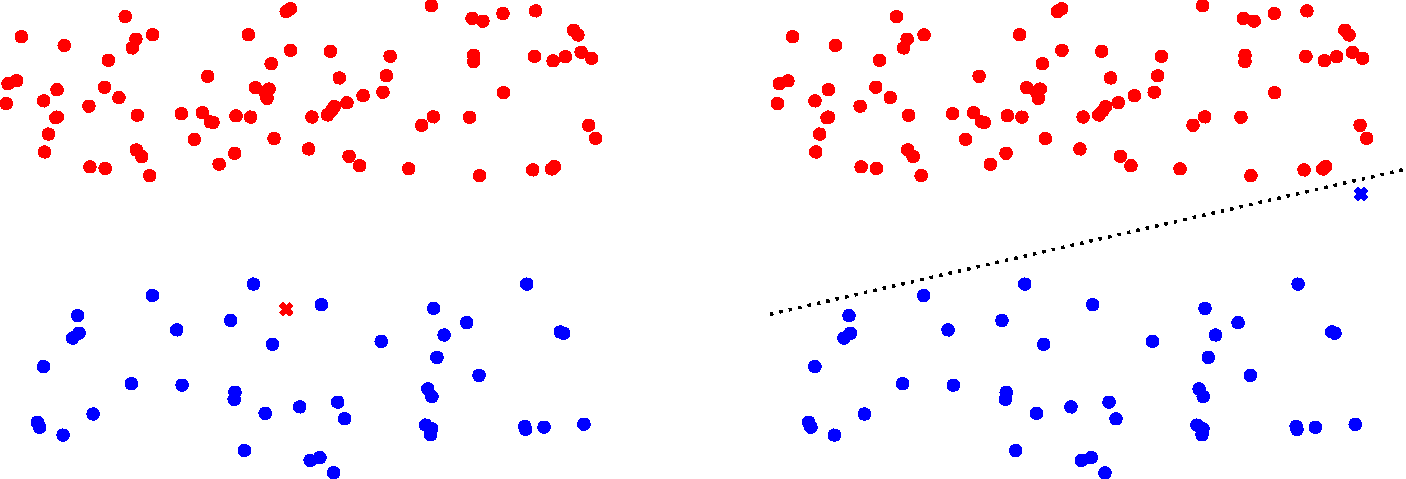
\includegraphics[width=\linewidth]{img/casi_dove_hardmargin_va_male_o_non_va.pdf}
    \caption{A sinistra un esempio di dataset non linearmente separabile, non risolvibile con il modello \emph{hard margin}. A destra un caso linearmente separabile la cui soluzione \emph{hard margin} è fortemente influenzata da un \emph{outlier}. I dati con segno ``X'' sono erroneamente etichettati.}
    \label{fig:svc:softmargin:casi_che_hardmargin_non_risolve}
\end{figure}
Per generalizzare il modello \emph{support vector classifier} e renderlo tollerante ad errori di classificazione, si riformula il problema di ottimizzazione in~\Cref{eq:svc:hardmargin:primal}, introducendo $m$ variabili di \emph{slack}/scarto $\xi_i \geq 0 \quad i=1,...,m$, una per ogni dato di addestramento. 
Ogni valore $\xi_i$ sarà proporzionale alla distanza tra $\Vec{x}_i$ erroneamente classificato e la superficie di separazione. 
La variabile $\xi_i$ sarà nulla per ogni $\Vec{x}_i$ correttamente classificato. Resta da definire come utilizzare le variabili di \emph{slack} per penalizzare la scelta di dati erroneamente classificati. 
In generale si definisce il problema primale
\begin{equation}
\begin{aligned}
& \min_{\Vec{w},b}    && \norm{\Vec{w}} + \frac{C}{p}\sum_{i=1}^{m}\xi_i^p\\
& \textrm{s.t.} && y_i(\Vec{w}\cdot\Vec{x}_i + b) \geq 1 - \xi_i, &&  i=1,\dots,m, \\
&               && \xi_i \geq 0,                 &&  i=1,\dots,m.\\
\end{aligned}
\end{equation}
Il parametro $C$, fissato a priori, determina il grado di tolleranza agli \emph{outlier}, bilanciando la funzione obiettivo originale con la penalità introdotta dalle variabili di \emph{slack}.
%
Il valore di $p$ è scelto tra $p=1$ (L1-SVC) e $p=2$ (L2-SVC). Viene qui considerata la formulazione L1-SVC:
\begin{equation}
\label{eq:svc:softmargin:primal}
\begin{aligned}
& \min_{\Vec{w},b,\Vec{\xi}}    && \norm{\Vec{w}} + C\sum_{i=1}^{m}\xi_i\\
& \textrm{s.t.} && y_i(\Vec{w}\cdot\Vec{x}_i + b) \geq 1 - \xi_i, &&  i=1,\dots,m, \\
&               && \xi_i \geq 0,                 &&  i=1,\dots,m.\\
\end{aligned}
\end{equation}
Il modello così modificato, viene chiamato \emph{soft margin support vector classifier}.
Si riporta in~\Cref{fig:soft_margin} un esempio di modello \emph{soft margin} per un insieme di dati su due dimensioni.

\begin{figure}
    \centering
    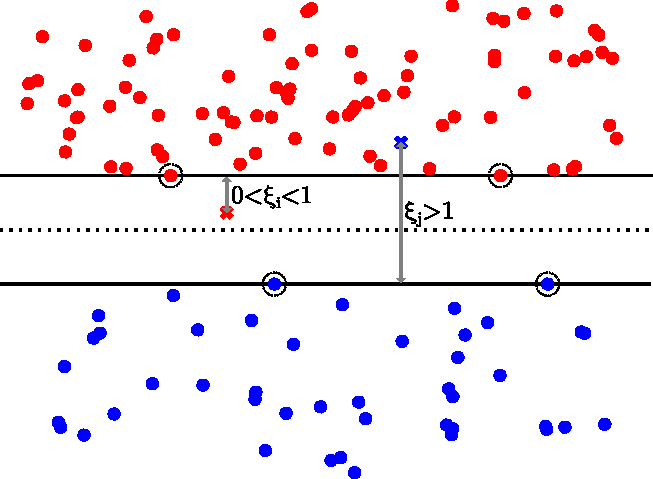
\includegraphics[width=.7\linewidth]{img/soft_margin.pdf}
    \caption{Con la formulazione \emph{soft margin} si tollerano esempi dalla parte sbagliata della superficie di separazione ($\xi_i>1$) o troppo vicini alla superficie di separazione ($0<\xi_i<1$). I punti in questione sono rappresentati in figura con un segno ``X''.}
    \label{fig:soft_margin}
\end{figure}



\subsection{Formulazione duale}\label{subsec:soft_margin_dual}
Il procedimento per ricavare la formulazione duale è analogo al caso \emph{hard margin}.
Si riscrive la funzione obiettivo del problema~\Cref{eq:svc:softmargin:primal} e si esprimono i vincoli in forma normale, ottenendo il problema
\begin{equation}
\label{eq:svc:softmargin:primal_convenient}
\begin{aligned}
& \min_{\Vec{w},b,\Vec{\xi}}    && \frac{1}{2}\norm{\Vec{w}}^2 + C\sum_{i=1}^{m} \xi_i \\
& \textrm{s.t.} && y_i(\Vec{w}\cdot \Vec{x}_i + b) - 1 + \xi_i \geq 0, && i=1,\dots,m, \\
&               && \xi_i \geq 0,  && i=1,\dots,m.
\end{aligned}
\end{equation}
%
Si applica il metodo dei moltiplicatori di Lagrange, ottenendo la funzione lagrangiana
\begin{equation}
\label{eq:svc:softmargin:lagrange_fn}
\begin{split}
L_P(\Vec{w},b, \Vec{\xi}, \Vec{\alpha}, \Vec{\mu}) = & \frac{1}{2}\norm{\Vec{w}}^2 + C\sum_{i=1}^{m} \xi_i - \sum_{i=1}^{m} \alpha_i (y_i(\Vec{w}\cdot \Vec{x}_i +b) -1 +\xi_i) - \sum_{i=1}^{m}\mu_i\xi_i =\\
        = & \frac{1}{2}\Vec{w}\cdot\Vec{w} + C\sum_{i=1}^{m} \xi_i - \sum_{i=1}^{m} \alpha_i y_i(\Vec{w}\cdot \Vec{x}_i +b) -  \sum_{i=1}^{m} - \alpha_i  \\ & - \sum_{i=1}^{m} \alpha_i\xi_i - \sum_{i=1}^{m}\mu_i\xi_i= \\
        = & \frac{1}{2}\Vec{w}\cdot\Vec{w} + C\sum_{i=1}^{m} \xi_i - \sum_{i=1}^{m} \alpha_i y_i \Vec{w}\cdot \Vec{x}_i - b \sum_{i=1}^{m} \alpha_i y_i \\ & + \sum_{i=1}^{m} \alpha_i - \sum_{i=1}^{m} \alpha_i\xi_i - \sum_{i=1}^{m}\mu_i\xi_i,
\end{split}
\end{equation}
da minimizzare rispetto a $\Vec{w},b,\Vec{\xi}$ e da massimizzare rispetto ad $\Vec{\alpha}, \Vec{\mu}$ 
\begin{equation}
\label{eq:svc:softmargin:max_min}
\begin{aligned}
& \max_{\Vec{\alpha}, \Vec{\mu}} \min_{\Vec{w}, b, \Vec{\xi}} && L_P(\Vec{w},b, \Vec{\xi}, \Vec{\alpha}, \Vec{\mu}) \\
& \textrm{s.t.} && \alpha_i \geq 0,  && i=1,..., m,\\
&               && \mu_i \geq 0,     && i=1,..., m.\\
\end{aligned}
\end{equation}
%
Una soluzione ottima per il problema in~\Cref{eq:svc:softmargin:max_min} deve soddisfare le condizioni di Karush-Kuhn-Tucker:
\begin{align}
    \label{eq:svc:softmargin:kkt1}
    \pd{L_P(\Vec{w},b, \Vec{\xi}, \Vec{\alpha}, \Vec{\mu})}{\Vec{w}} = \Vec{0},  \\[2mm]
    \label{eq:svc:softmargin:kkt2}
    \pd{L_P(\Vec{w},b, \Vec{\xi}, \Vec{\alpha}, \Vec{\mu})}{b} = 0, \\[2mm]
    \label{eq:svc:softmargin:kkt3}
    \pd{L_P(\Vec{w},b, \Vec{\xi}, \Vec{\alpha}, \Vec{\mu})}{\Vec{\xi}} = 0, 
\end{align}
\begin{align}
    \label{eq:svc:softmargin:kkt4}
    \alpha_i^*(y_i(\Vec{x}_i\cdot\Vec{w}^*+b^*)-1+\xi_i^*) = 0,  && i=1,\dots,m, \\[2mm] 
    \label{eq:svc:softmargin:kkt5}
    \mu_i^*\xi_i^* = 0, && i=1,\dots,m, \\[2mm] 
    \label{eq:svc:softmargin:kkt6}
    \alpha_i \geq 0, \mu_i \geq 0, \xi_i \geq 0, && i=1,\dots,m.
\end{align}
Le condizioni nelle~\Cref{eq:svc:softmargin:kkt1,eq:svc:softmargin:kkt2,eq:svc:softmargin:kkt3}, ovvero
\begin{equation*}
    \begin{split}
        \pd{L}{\Vec{w}} & = \Vec{w} - \sum_{i=1}^{m}\alpha_iy_i\Vec{x}_i = \Vec{0},\\
        \pd{L}{b} &=  \sum_{i=1}^{m}\alpha_iy_i = 0,\\
        \pd{L}{\Vec{\xi}} &= C -\sum_{i=1}^{m}\alpha_i - \sum_{i=1}^{m}\mu_i = 0,
    \end{split}
\end{equation*}
si riducono a
\begin{align} 
    \label{eq:svc_hard_sub1}
    \Vec{w} = \sum_{i=1}^{m}\alpha_iy_i\Vec{x}_i,  \\[2mm]
    \label{eq:svc_hard_sub2}
    \sum_{i=1}^{m}\alpha_iy_i = 0, \\[2mm]
    \label{eq:svc_hard_sub3}
    C = \sum_{i=1}^{m}\alpha_i + \sum_{i=1}^{m}\mu_i.
\end{align}
Sostituendo le~\Cref{eq:svc_hard_sub1,eq:svc_hard_sub2,eq:svc_hard_sub3} nella funzione~(\ref{eq:svc:softmargin:lagrange_fn}) si ottiene la funzione obiettivo duale
\begin{equation}
\begin{split}
L_D(\Vec{w},b, \Vec{\xi}, \Vec{\alpha}, \Vec{\mu}) = & \frac{1}{2}\Vec{w}\cdot\Vec{w} + C\sum_{i=1}^{m} \xi_i - \sum_{i=1}^{m} \alpha_i y_i \Vec{w}\cdot \Vec{x}_i - b \sum_{i=1}^{m} \alpha_i y_i \\ & + \sum_{i=1}^{m} \alpha_i - \sum_{i=1}^{m} \alpha_i\xi_i - \sum_{i=1}^{m}\mu_i\xi_i =\\
= & \frac{1}{2}\sum_{i=1}^{m}\alpha_iy_i\Vec{x}_i \cdot \sum_{i=1}^{m}\alpha_iy_i\Vec{x}_i  + \sum_{i=1}^{m}\alpha_i\xi_i + \sum_{i=1}^{m}\mu_i\xi_i \\
& - \sum_{i=1}^{m} \alpha_i y_i  \cdot \Vec{x}_i \sum_{j=1}^{m}\alpha_jy_j\Vec{x}_j + \sum_{i=1}^{m} \alpha_i - \sum_{i=1}^{m} \alpha_i\xi_i - \sum_{i=1}^{m}\mu_i\xi_i =\\
=& \frac{1}{2}\sum_{i=1}^{m}\sum_{j=1}^{m}\alpha_i\alpha_jy_iy_j\Vec{x}_i\cdot\Vec{x}_j + \sum_{i=1}^{m} \alpha_i,
\end{split}  
\end{equation}
espressa esclusivamente in funzione di $\Vec{\alpha}$.
Aggiungendo i rimanenti vincoli si ottiene la formulazione del problema duale
\begin{equation}\label{eq:svc:softmargin:wolfe_dual}
\begin{aligned}
& \max_{\vec{\alpha}}    && \sum_{i=1}^{m}\alpha_i - \frac{1}{2}\sum_{i=1}^{m}\sum_{j=1}^{m}\alpha_i\alpha_jy_iy_j\Vec{x}_i\cdot\Vec{x}_j\\
& \textrm{s.t.} && \sum_{i=1}^{m} \alpha_iy_i = 0, \\
&               && 0 \leq \alpha_i \leq C, && i=1,\dots,m. \\
\end{aligned}
\end{equation}
Come nel caso \emph{soft margin}, $\Vec{w}^*$ e $b^*$ sono ricavati dai vettori di supporto.
Si può notare come la formulazione duale \emph{hard margin} sia sostanzialmente identica alla formulazione duale \emph{soft margin}, con la differenza che in quest'ultima i moltiplicatori lagrangiani hanno un valore limitato al massimo a $C$.

% Dimitris Bertsimas, Jack Dunn, Colin Pawlowski, Ying Daisy Zhuo (2019) Robust Classification. INFORMS Journal on Optimization 1(1):2-34. https://doi.org/10.1287/ijoo.2018.0001 '' Both the primal and dual are convex quadratic optimization problems. Because the dual problem has fewer decision variables, and the majority of these variables tend to be equal to zero or the cost parameter C in the optimal solution, it is typically the problem solved in practice (Friedman et al. 2001). In addition, the dual form is ad vantageous because it allows us to do the kernel trick to learn nonlinear decision rules (Cortes and Vapnik 1995).''



\section{\emph{Kernel trick}}\label{sec:kernel_trick}
I modelli esposti fino ad ora sono dei classificatori lineari e non sono in grado di modellare relazioni più complesse.
Come anticipato nel~\Cref{sec:kernel_methods}, si può rendere il modello SVC non lineare utilizzando una funzione \emph{kernel}.

Si potrebbe pensare di elaborare i dati prima di addestrare un modello, applicando una trasformazione in grado di renderli linearmente separabili in un nuovo spazio.
Considerando per esempio i dati mostrati in~\Cref{fig:kerneltrick:non_lin_sep}, non linearmente separabili nello spazio monodimensionale originale, si potrebbe ipotizzare di applicare una trasformazione utilizzando la funzione $\Phi:\mathbb{R} \rightarrow \mathbb{R}^2,$ con $\Phi(x) = (x, x^2)$, ottenendo un nuovo insieme di dati linearmente separabili nel nuovo spazio, mostrato in~\Cref{fig:kerneltrick:visualized}. 

\begin{figure}
    \begin{subfigure}[t]{.45\textwidth}
        \centering
        
\includegraphics[width=\textwidth]{img/non_linearmente_separabili.pdf}
        \caption{Insieme di dati non linearmente separabili nello spazio originale. Il colore identifica la classe di ogni punto.}
        \label{fig:kerneltrick:non_lin_sep}
    \end{subfigure}%
    \hfill
    \begin{subfigure}[t]{.45\textwidth}
        \centering
        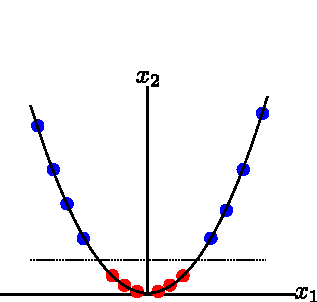
\includegraphics[width=\textwidth]{img/kernel_trick_visualized.pdf}
        \caption{I dati della~\Cref{fig:kerneltrick:non_lin_sep}, mappati nel nuovo spazio bidimensionale, sono linearmente separabili (per esempio dalla retta tratteggiata).}
        \label{fig:kerneltrick:visualized}
    \end{subfigure}%
    \caption{Esempio di trasformazione per rendere un insieme di dati linearmente separabili in un nuovo spazio.}
\end{figure}

% \begin{figure}
%     \centering
%     
\includegraphics[width=0.5\linewidth]{img/non_linearmente_separabili.pdf}
%     \caption{Esempio in una dimensione di dati non linearmente separabili. Il colore identifica la classe di ogni punto.}
%     \label{fig:kerneltrick:non_lin_sep}
% \end{figure}
% \begin{figure}
%     \centering
%     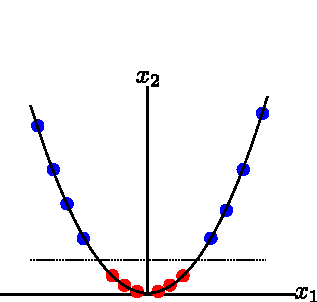
\includegraphics[width=0.5\linewidth]{img/kernel_trick_visualized.pdf}
%     \caption{I dati della~\Cref{fig:kerneltrick:non_lin_sep}, mappati nel nuovo spazio bidimensionale, sono linearmente separabili (per esempio dalla retta tratteggiata).}
%     \label{fig:kerneltrick:visualized}
% \end{figure}

In generale, si vorrebbero mappare i dati di addestramento dallo spazio originale $\mathcal{X}$ ad uno spazio delle \emph{feature} $\mathcal{H}$ di dimensioni maggiori, potenzialmente infinite, usando una funzione
\begin{equation}
\label{eq:generic_kernel_mapping}
\Phi(x_i) : \mathcal{X} \rightarrow \mathcal{H}
\end{equation}
in modo da rendere i dati linearmente separabili in $\mathcal{H}$.


Rifacendosi alla formulazione del problema \emph{soft margin} in~\Cref{eq:svc:softmargin:wolfe_dual} è possibile notare come i dati di addestramento compaiano nella funzione obiettivo esclusivamente come prodotto scalare tra di essi. 
Per applicare esplicitamente la trasformazione $\Phi$, si dovrebbe dunque calcolare $\Phi(\Vec{x}_i)\cdot\Phi(\Vec{x}_j)$ per $i=1,\dots,m$, il che renderebbe la procedura costosa dal punto di vista computazionale, se non impossibile ($\mathcal{H}$ di infinite dimensioni). 
Come anticipato nel~\Cref{sec:kernel_methods}, è possibile esprimere il prodotto scalare tra elementi appartenenti ad $\mathcal{H}$ con una funzione espressa in termini di prodotto scalare tra elementi di $\mathcal{X}$. 
Esiste la funzione \emph{kernel}
\begin{equation*}
    K: \mathcal{X} \times \mathcal{X} \rightarrow \mathbb{R} 
\end{equation*}
per cui per ogni $\Vec{x}_i, \Vec{x}_j \in \mathcal{X}$ vale
\begin{equation*}
    K(\Vec{x}_i, \Vec{x}_j) = \Phi(\Vec{x}_i) \cdot \Phi(\Vec{x}_j).
\end{equation*}
Il \emph{kernel trick} consiste nell'utilizzare una funzione \emph{kernel} $K$ in modo che la funzione $\Phi$ non debba essere calcolata esplicitamente. 
La funzione $K$, utilizzando i dati nello spazio originale, calcola un risultato equivalente al prodotto scalare tra i punti trasformati. 
Il valore $K(\Vec{x}_i, \Vec{x}_j)$ può essere interpretato come una misura della ``vicinanza'', o meglio come una una misura di similarità, tra i punti $\Vec{x}_i, \Vec{x}_j$.
Esistono diverse funzioni \emph{kernel}; le più utilizzate sono riportate nell'elenco seguente:
\begin{itemize}
    \item Kernel lineare, calcolato come
    \begin{equation*}
        K(\Vec{x}_1, \Vec{x}_2) = \Vec{x}_1\cdot\Vec{x}_2.
    \end{equation*} 
    Questo \emph{kernel} è in realtà fittizio perché la $\Phi$ corrispondente equivale all'identità $\Phi(\Vec{x}_i)=\Vec{x}_i$. Utilizzare il \emph{kernel} lineare produce un modello lineare nello spazio originale.
    \item Kernel polinomiale, calcolato come
    \begin{equation*}
        K(\Vec{x}_1, \Vec{x}_2) = (\Vec{x}_1\cdot\Vec{x}_2 + 1)^d.
    \end{equation*} 
    Questo \emph{kernel} trasforma i vettori in uno spazio a dimensione finita. L'iperparametro $d$ viene fissato a priori. Utilizzando questo \emph{kernel}, l'iperpiano di separazione nello spazio delle \emph{feature} induce una superficie di separazione nello spazio originale che corrisponde ad una superficie polinomiale di grado al massimo uguale a $d$.
    \item Kernel gaussiano, calcolato come:
    \begin{equation*}
        K(\Vec{x}_1, \Vec{x}_2) = \mathrm{exp}({-\frac{\norm{\Vec{x}_1 - \Vec{x}_2}^2}{2 \sigma^2}}).
    \end{equation*} 
    Questo \emph{kernel} trasforma i vettori in uno spazio di dimensione infinita. L'iperparametro $\sigma$ viene fissato a priori. Utilizzando questo \emph{kernel}, l'iperpiano di separazione nello spazio delle \emph{feature} induce una superficie di separazione nello spazio originale che corrisponde ad una somma di distribuzioni gaussiane multivariate con deviazione standard $\sigma$.
\end{itemize}
%
In generale, le condizioni per far sì che una funzione $K$ sia un \emph{kernel}, derivano da un noto teorema di Mercer\cite{mercer_theorem, RKHS}. Se la funzione \emph{kernel} $K$ è simmetrica, continua e definita semi-positiva, allora esiste una funzione 
\begin{equation}
    \Phi(x) : \mathbb{R}^p \rightarrow \mathcal{H}
\end{equation} 
tale per cui 
\begin{equation*}
    K(\Vec{x}_i, \Vec{x}_j) = \Phi(\Vec{x}_i)\cdot\Phi(\Vec{x}_j).
\end{equation*} 
L'introduzione del \emph{kernel trick} modifica il problema in~\Cref{eq:svc:softmargin:wolfe_dual}, che diventa quindi
\begin{equation}\label{eq:svc:softmargin:wolfe_dual_plus_kernel_trick}
\begin{aligned}
& \max_{\vec{\alpha}}    && \sum_{i=1}^{m}\alpha_i - \frac{1}{2}\sum_{i=1}^{m}\sum_{j=1}^{m}\alpha_i\alpha_jy_iy_jK(\Vec{x}_i, \Vec{x}_j)\\
& \textrm{s.t.} && \sum_{i=1}^{m} \alpha_iy_i = 0, \\
&               && 0 \leq \alpha_i \leq C, && i=1,\dots,m. \\
\end{aligned}
\end{equation}
%
La predizione della classe di un nuovo esempio $\Vec{x}_\text{test}$ sarà ottenuta calcolando 
\begin{align*}
h(\Vec{x}_\text{test})  &= \sign(\Vec{w}^*\cdot\Phi(\vec{x}_{text}) +b^*) =\\
                        &= \sign\left(\sum_{i\in S} \alpha_i^*y_i \Phi(\vec{x}_i) \cdot \Phi(\vec{x}_{text}) + b^*\right)=\\
                        &= \sign\left(\sum_{i \in S}\alpha_i^*y_iK(\Vec{x}_i, \Vec{x}_\text{test}) + b^*\right)
\end{align*}

In uno spazio con più dimensioni rispetto all'originale, è sempre possibile trovare un margine di separazione in grado di dividere i dati delle due classi perfettamente. % sempre anche con una sola dimensione in più. e.g. phi([x1]) -> [x1,y1] dove y1 è il label.
Pur essendo un risultato più preciso dal punto di vista del problema di ottimizzazione, potrebbe invece causare \emph{overfitting}. Rimane dunque cruciale la scelta del parametro $C$. 
Per valori di $C$ troppo alti, il modello cercherà di adattarsi troppo fedelmente ai dati di addestramento, creando una superficie di separazione inutilmente complessa nello spazio originale e con pessime capacità di generalizzazione. 
Al contrario, un valore basso di $C$ porterà ad una superficie di separazione più semplice e regolare, bilanciando però con più errori di classificazione. 
Per trovare un valore di $C$ soddisfacente, raggiungendo un buon compromesso tra complessità della superficie di separazione ed errori di classificazione, si utilizzano in genere delle tecniche di \emph{model selection} (viste nel~\Cref{sec:model_selection}).  


\section{Limitazioni}\label{sec:svc_limiti}
I \emph{support vector classifier} presentano alcune limitazioni di cui serve tener conto. 
Sono modelli suscettibili alla presenza di \emph{outlier}, intesi come dati erroneamente classificati o rumore. L'approccio \emph{soft-margin} consente di trattare anche problemi di questo tipo, ma la soluzione trovata potrebbe comunque subire (in misura variabile) l'effetto degli \emph{outlier}, dato che ognuno di questi punti diventerà un vettore di supporto con una relativa variabile di \emph{slack} che influirà sul valore della funzione obiettivo. 
Di conseguenza, i modelli SVC addestrati su dataset con rumore hanno in genere performance peggiori rispetto ad altri tipi di modelli pensati specificatamente per dati con molti outlier, per esempio approcci chiamati \emph{robusti} \cite{2019_robust_classification}.
La presenza di rumore nel dataset è comunque un problema comune a tutti i modelli di apprendimento automatico e non riguarda solo i modelli \emph{support vector machine}.

Una seconda limitazione riguarda la scalabilità. La procedura di addestramento considera tutti i dati disponibili e risulta quindi troppo costosa da eseguire su grandi quantità di dati, o su dati con un alto numero di feature, pur utilizzando un algoritmo di ottimizzazione numerica efficiente, come \emph{sequential minimal optimization} \cite{SMO}.

Una terza limitazione riguarda la selezione dei parametri di addestramento: il costo $C$ e la funzione \emph{kernel}. La scelta ottimale di questi valori richiede in genere molteplici esecuzioni dell'algoritmo di addestramento, moltiplicando i tempi necessari.

Risultano motivati dunque tutti gli approcci che tentano di risolvere queste limitazioni. 


    \chapter{Sparse Support Vector Classifier}\label{chap:sparse_svc}
In questo capitolo si presenta un'analisi dei metodi proposti in letteratura per ottenere modelli SVC con un numero ridotto di vettori di supporto, chiamati \emph{sparse SVC} o in generale \emph{sparse SVM}.
I modelli SVM nella formulazione originale sono già di per sé considerati modelli parsimoniosi, dato che utilizzano un sottoinsieme dei dati di addestramento per eseguire predizioni. 
Si utilizza comunque il termine \emph{sparse SVM} per indicare approcci che promuovono la parsimonia dei vettori di supporto e consentono in alcuni casi di impostare esplicitamente un limite al numero di vettori di supporto. 
Gli approcci presenti in letteratura sono vari e numerosi:
nel~\Cref{sec:sparsesvm:post_processing} si espongono alcuni approcci per ridurre il numero di vettori di supporto di un modello \emph{a posteriori}, ad addestramento già effettuato; nel~\Cref{sec:sparsesvm:on-line} si espongono alcuni approcci per l'addestramento \emph{on-line}; nel~\Cref{sec:sparsesmv:off-line} si espongono alcuni approcci per l'addestramento \emph{off-line}; nel~\Cref{sec:sparsesvm:feature-selection} si espongono dei metodi per eseguire \emph{feature selection} durante la procedura di addestramento; infine, nel~\Cref{sec:our_budgeted_svm} si descrive l'approccio proposto in questa tesi per produrre modelli SVC parsimoniosi.

\section{Riduzione post addestramento}\label{sec:sparsesvm:post_processing}
Tra i primi metodi presenti in letteratura per ridurre il numero di vettori di supporto si trovano degli approcci che modificano classificatori già addestrati. 
Rientra in questa categoria il \emph{reduced set method}~\cite{reduced_set_method}.
Si consideri un classificatore già addestrato con un kernel $K$ (corrispondente ad una funzione $\Phi$) su dati presi dal dominio $\mathcal{X}=\mathbb{R}^k$. Gli indici dei dati utilizzati come vettori di supporto sono contenuti nell'insieme $S$, definito nel~\Cref{subsec:hard_margin_dual}: si definisce $N_s=|S|$. 
La predizione della classe per un punto $\Vec{x}_\text{new}$ mai visto in fase di addestramento dipende dalla quantità
\begin{equation}\label{eq:before_reduced_set}
\Vec{w}^*\cdot\Phi(\Vec{x}_\text{new}) = \sum_{i=1}^{S} \alpha^*_iy_i\Phi(\Vec{x}_i) \cdot \Phi(\Vec{x}_\text{new}) = \sum_{i=1}^{S} \alpha^*_iy_iK(\Vec{x}_i, \Vec{x}_\text{new})
\end{equation}
dove gli $\alpha^*_i$ sono i moltiplicatori lagrangiani ottimi. 
Il \emph{reduced set method} consiste nell'identificare un insieme di punti $\Vec{z}_a \in \mathcal{X}$ con $a=1,\dots,N_z$ e dei corrispettivi pesi $\gamma_a \in \mathbb{R}$ che identificano 
\begin{equation*}
    \Vec{w}^{'} = \sum_{a=1}^{N_z}\gamma_a\cdot\Phi(\Vec{z}_a),
\end{equation*} 
tale per cui la distanza 
\begin{equation}\label{eq:reduced_set_p_distance}
    p = ||\Vec{w}^*-\Vec{w}^{'}||
\end{equation} 
sia minima. Si ottiene quindi con $\Vec{w}^{'}$ un'approssimazione della superficie di separazione originale.
L'insieme delle coppie $\{\gamma_a, \Vec{z}_a\}$, $a=1,\dots, N_z$ è il \emph{reduced set}, un insieme di elementi e corrispettivi moltiplicatori sintetici, per cui si può rimpiazzare l'~\cref{eq:before_reduced_set} con 
\begin{equation}\label{eq:reduced_set}
\Vec{w}^{'} \cdot \Phi(\Vec{x}_\text{new}) = \sum_{a=1}^{N_z}\gamma_a \Phi(\Vec{z}_a) \cdot \Phi(\Vec{x}_\text{new}) = \sum_{a=1}^{N_z}\gamma_a K(\Vec{z}_a, \Vec{x}_\text{new}).
\end{equation}
Idealmente si vorrebbe trovare un \emph{reduced set} di dimensione $N_z \ll N_s$ per cui le performance degradino di una quantità accettabile, potenzialmente nulla.
Nella pratica trovare il \emph{reduced set} significa minimizzare la distanza $p$ in~\Cref{eq:reduced_set_p_distance}. 
In altre parole il \emph{reduced set method} rimpiazza i vettori di supporto originali e i corrispettivi moltiplicatori lagrangiani con una quantità idealmente molto ridotta di vettori di supporto sintetici ed altrettanti moltiplicatori ``lagrangiani'' sintetici. 
%TODO: è giusto lasciare le virgolette? Perché non sono tecnicamente moltiplicatori lagrangiani? no?

Si trova in~\cite{burges_improving_accuracy} un approccio che combina il \emph{reduced set method} con un ulteriore \emph{virtual support vector method}, che consiste nell'introdurre delle invarianti note relative al problema trattato, applicando una trasformazione ai vettori di supporto trovati dopo il primo addestramento del modello. 
Combinando queste due tecniche, gli autori ottengono un miglioramento nelle capacità di generalizzazione ed un miglioramento dell'efficienza in fase di predizione. Le migliori capacità di generalizzazione sono merito del \emph{virtual support vector method}; l'efficienza in fase di predizione è merito del \emph{reduced set method}.
Questo approccio richiede però una conoscenza specifica relativa al problema trattato che consenta di applicare una trasformazione sensata sui vettori di supporto. Non vengono fornite delle trasformazioni generiche applicabili su qualsiasi tipo di dato. 

Un approccio simile al \emph{reduced set method}, ma meno oneroso dal punto di vista computazionale, è quello proposto in~\cite{2005_merging_strategy}, dove coppie di vettori di supporto originali sono iterativamente sostituite da un singolo vettore di supporto sintetico, a seconda di particolari condizioni. 

Un altro metodo per ridurre il numero di vettori di supporto è quello proposto in~\cite{1998_reducing_svm_complexity}:
sempre in seguito all'addestramento di un modello, si rimuovono i vettori di supporto che contribuiscono a rendere la superficie di separazione troppo contorta, utilizzando un modello \emph{support vector regression machine} (SVRM) per approssimare la superficie di separazione originale.
Per risolvere questo problema di regressione si suggerisce di utilizzare lo stesso kernel utilizzato per addestrare il modello di classificazione.
L'approccio è simile al \emph{reduced set method} ma è meno vantaggioso nei casi in cui i moltiplicatori $\alpha$ siano strettamente nell'intervallo $[0,C]$, oppure in generale quando la superficie di separazione è particolarmente contorta nello spazio delle \emph{feature}.

Si descrive in~\cite{2005_multistage_postprocessing} una riduzione in \emph{post-processing} più aggressiva, composta da quattro fasi. 
Nella prima fase si addestra un classificatore sull'intero insieme di dati. 
Nella seconda fase si rimuovono dai dati di addestramento tutti i vettori di supporto le cui proiezioni sulla superficie di separazione abbiano la curvatura maggiore. 
Nella terza fase si addestra un secondo classificatore utilizzando i dati di addestramento modificati nella fase precedente. 
Nell'ultima fase si adotta l'approccio descritto in~\cite{1998_reducing_svm_complexity}, approssimando ulteriormente la superficie di separazione utilizzando un modello SVRM.

In generale, questa classe di approcci è efficace nel migliorare l'efficienza dei modelli ma non migliora i tempi di calcolo della fase di addestramento, dato che sono richiesti molteplici passaggi in aggiunta ad un modello SVC classico, che già di per se è comunemente addestrato più volte per trovare i migliori iperparametri.

\section{Riduzione con addestramento on-line}\label{sec:sparsesvm:on-line}
I \emph{support vector classifier} possono essere usati anche per addestramento \emph{on-line}, scenario in cui i dati di addestramento sono forniti col passare del tempo. 
Considerando che la quantità di dati d'addestramento non è nota \emph{a priori}, risulta fondamentale inserire delle tecniche per contenere il numero di vettori di supporto, che tipicamente cresce linearmente rispetto al numero di dati di addestramento~\cite{2003_online_classification_on_a_budget}. 
Questa problematica è chiamata in letteratura \emph{curse of kernelization}~\cite{2012_bsgd}. 
Per questo motivo esistono numerosi approcci per promuovere la parsimonia dei vettori di supporto dei modelli addestrati con approccio \emph{on-line}.

Per tutti questi metodi si utilizza comunque il termine \emph{vettore di supporto} anche se in realtà non si tratta necessariamente di punti del \emph{\emph{dataset}} di addestramento con coefficienti lagrangiani non nulli ma semplicemente di punti del \emph{\emph{dataset}} (o punti fittizi) che contribuiscono alla definizione della superficie di separazione.

L'algoritmo \emph{perceptron}~\cite{1958_perceptron} è un algoritmo di addestramento \emph{on-line} originariamente utilizzato per addestrare il modello omonimo (reti neurali con un solo neurone), ma che può essere usato per addestrare modelli \emph{support vector machine}.
In~\cite{2003_online_classification_on_a_budget} si descrive una variante che mantiene un insieme di dimensione variabile dei vettori di supporto. 
Viene battezzata \emph{variable size cache} perché non viene imposto un limite fisso alla sua dimensione (\emph{variable size} appunto) e gli elementi già presenti possono essere rimossi secondo una strategia adatta, proprio come una \emph{cache} generica. 
Questi algoritmi di gestione della \emph{cache} vengono ripresi in lavori successivi, per esempio in~\cite{2012_bsgd} (poi utilizzato per effettuare esperimenti descritti nel~\cref{sec:comparazione_metodi}).
Formalmente, per una generica variante di \emph{perceptron on-line}, al tempo $t$ l'algoritmo riceve un nuovo dato $\Vec{x}_t$ con la corrispettiva etichetta $y_t$: si calcola $s_t = \sum_{i<t} \alpha_iy_iK(\Vec{x}_i, \Vec{x}_t)$ da cui si ricava la predizione $\sign(s_t)$. 
L'algoritmo \emph{perceptron} nella forma originale usa come iperparametri $\beta_t=0, \alpha_t=1, c_t=1$. 
Per decidere se $\Vec{x}_t$ debba essere selezionato come nuovo vettore di supporto si valuta la condizione $y_ts_t \leq \beta_t$.
La strategia per effettuare questa aggiunta dipende dall'algoritmo specifico. 
Per prima cosa, serve assegnare un valore ad $\alpha_t$ (che non necessariamente è fisso). 
Si modifica poi la superficie di separazione $\Vec{w}_{t+1} = \Vec{w}_t + \alpha_ty_t\Vec{x}_t$. 
L'ultimo passo (``opzionale'') consiste nello scalare il vettore $\Vec{w}_{t+1} \leftarrow c_t\Vec{w}_{t+1}$ per un certo $c_t > 0$. 

Per limitare il numero di vettori di supporto, una volta aggiunto $\Vec{x}_t$, vengono rimossi tutti gli $\Vec{x}_i$ per cui $y_i(\Vec{w} - \alpha_iy_i\Vec{x}_i)\leq \beta_t$. 
Questo approccio non impone una dimensione fissa alla \emph{cache} e richiede di ricalcolare per ogni vettore di supporto già presente, la condizione di mantenimento ad ogni nuova possibile aggiunta. 
Sempre in~\cite{2003_online_classification_on_a_budget} viene definito un limite teorico alla dimensione della \emph{cache}: la dimensione della \emph{cache} è inversamente proporzionale al quadrato del miglior margine ottenibile sui dati visti fino a quel momento.

Seguendo approcci analoghi sono state proposte negli anni diverse varianti dell'algoritmo \emph{perceptron}.

In~\cite{2005_forgetron} si introduce il \emph{forgetron}, una variante che utilizza un altro criterio per la rimozione dei vettori di supporto. 
Al tempo $t$, se $\Vec{x}_t$ viene classificato erroneamente, si aggiornano i vettori di supporto in tre passaggi: si esegue inizialmente l'algoritmo perceptron classico; si scalano in seguito i coefficienti dei vettori di supporto; si rimuovono infine i vettori di supporto con il coefficiente più piccolo.

Si introduce in~\cite{2007_random_removal} il \emph{random perceptron}, una variante in cui la rimozione di un vettore di supporto viene effettuata casualmente.

I metodi in~\cite{2003_online_classification_on_a_budget,2005_forgetron,2007_random_removal} usano la strategia di rimozione dei vettori di supporto ma con criteri diversi.

Si introduce in~\cite{2008_projectron} il \emph{projectron}, una variante che utilizza una strategia di proiezione: un punto viene aggiunto come vettore di supporto se la sua proiezione sulla copertura lineare~\cite{2008_projectron} nello spazio delle \emph{feature} eccede un limite definito \emph{a priori}. 
%``The new vector is added to the support set if its projection onto the linear span of others in the feature space exceeds a predefined threshold, or otherwise its information is kept through the projection.''
%

In alternativa alle strategie di rimozione o proiezione, è possibile utilizzare una strategia di unione, dove coppie di vettori di supporto vengono approssimate da un singolo vettore di supporto.
Questo approccio deriva dalla procedura descritta in~\cite{2005_merging_strategy}.

Si trovano poi in letteratura degli approcci diversi per addestramento \emph{on-line}, non basati sull'algoritmo \emph{perceptron}.

In~\cite{2012_bsgd} si combina il metodo di risoluzione del problema primale per SVM basato su discesa del gradiente~\cite{2007_chappelle_training_svm_primal, pegasos_solver} con le strategie di mantenimento dell'insieme di vettori di supporto rimozione, proiezione e unione viste in precedenza. 
Il risultato è un algoritmo risolutivo efficiente, pensato principalmente per problemi \emph{on-line}, che fornisce la possibilità di esprimere \emph{a priori} un numero massimo di vettori di supporto.

In~\cite{2017_approximation_vm} si introduce il modello \emph{approximation vector machine}. 
L'idea è quella di non considerare ogni punto di addestramento a sé stante, ma raggruppare automaticamente  i dati in \emph{cluster}. 
Ogni nuovo punto è approssimato da un ``centroide'' che si trova nello spazio delle \emph{feature} entro una distanza massima dal nuovo punto. 
Una caratteristica aggiuntiva è quella di non richiedere \emph{a priori} il numero di vettori di supporto massimo come iperparametro.
La motivazione per questo approccio è che in un contesto \emph{on-line} non è possibile sapere \emph{a priori} la dimensione totale del \emph{dataset} e di conseguenza sarebbe molto difficile impostare un valore di \emph{budget} sensato. 


\section{Riduzione con addestramento off-line}\label{sec:sparsesmv:off-line}
Tutti gli approcci visti nel~\Cref{sec:sparsesvm:on-line} per l'addestramento \emph{on-line} possono essere adattati per un approccio \emph{off-line}, per esempio fornendo il set di addestramento come uno \emph{stream} artificiale di dati.
Rimane comunque sensato sviluppare approcci dedicati per addestramento off-line, cercando di sfruttare la disponibilità dell'intero \emph{dataset} come un vantaggio e non come una limitazione.

Molti approcci per la riduzione del numero di vettori di supporto durante l'addestramento \emph{off-line} si basano sull'osservazione che i vettori di supporto corrispondenti a dati erroneamente etichettati, ovvero vettori di supporto con le rispettive variabili di scarto non nulle, influiscono negativamente sul valore della funzione obiettivo, oltre che richiedere spazio per essere memorizzati e influire sul costo computazionale di ogni predizione. 
Un approccio per ridurre l'effetto degli \emph{outlier} è la formulazione del problema chiamata L2-SVC accennata nel~\Cref{sec:soft_margin_classifier}:
\begin{equation}
\label{eq:l2svc}
\begin{aligned}
& \min_{w,b}    && \frac{1}{2}\norm{\Vec{w}}^2 + \frac{C}{2}\sum_{i=0}^{m} \xi_i^2 \\
& \textrm{s.t.} && y_i(\Vec{w}\cdot \Vec{x}_i + b) - 1 + \xi_i \geq 0, && i=1,\dots,m, \\
&               && \xi_i \geq 0,  && i=1,\dots,m.
\end{aligned}
\end{equation}
Le variabili di scarto compaiano nella funzione obiettivo elevate al quadrato: 
la selezione di vettori di supporto con relative variabili di scarto $>1$ è penalizzata maggiormete rispetto alla formulazione L1-SVC classica.
Si riportano in questo paragrafo alcuni approcci simili presenti in letteratura, approcci in cui si modifica il termine della funzione obiettivo relativo alle variabili di scarto.

Si trova in~\cite{2005_penalizing_outliers} una procedura di addestramento basata sull'osservazione che l'iperpiano di separazione tra le due classi viene reso inutilmente complicato a causa di \emph{outlier}. 
Per limitarne l'effetto, si riformula la funzione obiettivo del problema primale vista nell'~\Cref{eq:svc:softmargin:primal_convenient}, introducendo una funzione di penalità non lineare sulle variabili di scarto. Il risultato è il problema
\begin{equation}\label{eq:adaptively_penalizing_outliers}
\begin{aligned}
& \min_{\Vec{w}}    && \frac{1}{2}\norm{\Vec{w}}^2 +C \sum_{i=1}^{m}\mathrm{erf}(\xi_i, \sigma) \\
& \textrm{s.t.}     && y_i(\Vec{w}\cdot\Phi(\Vec{x}_i) + b) \geq 1 -\xi_i, && i=1,\dots,m,\\
&                   && \xi_i \geq 0,  && i=1,\dots,m,
\end{aligned}
\end{equation}
dove la funzione di penalità $\mathrm{erf}$ è proposta come
\[
\mathrm{erf}(\xi, \sigma) = \frac{2}{\sqrt{\pi}\sigma} \int_{0}^{\xi}e^{\frac{-z^2}{\sigma^2}} dz.
\]
%
Il problema~\Cref{eq:adaptively_penalizing_outliers} si può comunque risolvere considerando la rispettiva formulazione duale, rendendo questo approccio relativamente facile da implementare e trattare con tecniche note, per esempio modificando \emph{sequential minimal optimization} (SMO)~\cite{SMO}.

% \cite{2001_ssvm_smooth_svm} propone di rimpiazzare la norma l1 delle variabili di scarto nella funzione obiettivo del problema primale \emph{soft-margin} con il quadrato della norma l2. Per rendere la funzione obiettivo doppiamente differenziabile (?) utilizza una smooth approximation function (?) così il problema può essere risolto con un fast newton method (?). 

Si introduce in~\cite{2006_svm_on_a_budget} una formulazione in grado di minimizzare l'errore prodotto dai $B$ punti peggio classificati, con $B$ iperparametro fissato \emph{a priori}. 
In questa variante solo $B$ esempi con variabile di scarto non nulla influiscono sulla funzione obiettivo, mentre eventuali ulteriori esempi con variabile di scarto non nulla vengono ignorati.
Si definisce un meta-algoritmo per derivare delle formulazioni concrete del problema SVC che utilizzano delle \emph{interpolation norm}~\cite{norm_interpolation} in sostituzione alle classiche norme 1 e 2. 
Il problema ottenuto applicando questa procedura alla formulazione L1-SVM è risolvibile con l'algoritmo \emph{SMO}~\cite{SMO}.

Esistono poi diversi approcci in letteratura che cercano di ridurre il numero di vettori di supporto in generale, senza concentrarsi in particolar modo sugli esempi con variabile di scarto non nulla.

% Viene introdotto in~\cite{2001_relevance_vector_machine} il modelo \emph{relevant vector machine}, un approccio non limitato ai modelli SVM per produrre soluzioni sparse.

La risoluzione classica del problema SVC vista nel~\Cref{chap:SVC} richiede di calcolare la \emph{matrice kernel} di dimensione $m\times m$, definita come $K(X,X)$ dove $X$ è l'insieme dei dati di addestramento, $K$ è la funzione \emph{kernel} e $m=|X|$. 
Ogni elemento in posizione $i,j$ è calcolato come $K(\Vec{x}_i, \Vec{x}_j)$. 
Calcolare i valori di questa matrice è oneroso per un insieme di dati sufficientemente grande sia in termini di calcolo che di memorizzazione. 
In~\cite{2001_rsvm} si introduce il modello \emph{reduced support vector machine} (RSVM): l'idea alla base è quella di ridurre la dimensione della matrice \emph{kernel}, considerando invece una matrice $K(X,X^{'})$ dove $X^{'} \subset X$ con $|X^{'}| \ll m$. 
La scelta degli elementi di $X^{'}$ è casuale. 
Si trova in~\cite{2003_rsvm_comparison} un'analisi più pratica del modello RSVM, messo a confronto con l'implementazione dei modelli SVM classici più utilizzata, LibSVM\cite{libsvm}.

Si propone in~\cite{2005_SLMC} il modello \emph{sparse large margin classifier} (SLMC). 
Dopo aver fissato $N_z$ uguale al numero di vettori di supporto desiderato, vengono introdotte le variabili $\Vec{Z} = \{\Vec{z_i}, i=1,\dots,N_z\}$ con la stessa dimensionalità dei dati di addestramento originali e $\Vec{\beta} = \{\beta_i \in \mathbb{R}, i=1,\dots,N_z\}$.
Viene così modificato il problema SVC \emph{soft margin} in~\Cref{eq:svc:softmargin:primal_convenient} aggiungendo un nuovo vincolo
\begin{equation*}
    \Vec{w} = \sum_{i=1}^{N_z} \Phi(\Vec{z}_i) \cdot \Vec{\beta}.
\end{equation*}
Le variabili $\Vec{z}_i$ e corrispettivi $\beta_i$ ricordano i ``vettori di supporto sintetici'' e corrispettivi moltiplicatori utilizzati nel \emph{reduced set method}, con la differenza che in questo caso sono introdotti direttamente come variabili nel problema di ottimizzazione originale, invece che essere calcolati in \emph{post-processing}.
Questa nuova formulazione non è convessa e viene risolta nell'articolo originale con un metodo del gradiente.

%**Building Support Vector Machines with Reduced Classifier Complexity** ma non ho capito cosa fa.

In~\cite{2012_LLSVM} si introduce un metodo che utilizza una matrice \emph{kernel} approssimata, trattata come scomposizione in matrici di dimensioni molto ridotte, su cui verrà poi addestrato un modello lineare, composto da un numero ridotto di vettori di supporto (se confrontato con un modello addestrato sulla matrice \emph{kernel} completa).

Si introduce in~\cite{2020_sparse_svm} l'approccio NSSVM, che propone un algoritmo basato su \emph{Newton method} per risolvere il problema
\begin{equation*}
\begin{aligned}
& \min_{\vec{w}, b}     && \frac{1}{2}\sum_{i=1}^{m}\sum_{j=1}^{m}\alpha_i\alpha_jy_iy_jK(\Vec{x}_i, \Vec{x}_j) - \sum_{i=1}^{m}\alpha_i + \sum_{i=1}^{m} h_{cC}(\alpha_i)\\
&\textrm{s.t.}          && \sum_{i=1}^{m}\alpha_iy_i=0, \\
&                       && \norm{\Vec{\alpha}}_0 \leq B,
\end{aligned}
\end{equation*}
dove $B$ è il numero massimo di vettori di supporto desiderato, $h_{cC}$ è una funzione di perdita definita come
\begin{equation*}
h_{cC}(t) = \begin{cases}
            t^2/(2C) & \text{se} \quad t \geq 0, \\
            t^2/(2c) & \text{se} \quad t < 0, \\
            \end{cases}
\end{equation*}
con $c,C$ iperparametri scelti e $\norm{\Vec{\alpha}}_0$ è la norma 0 di $\Vec{\alpha}$, ovvero il numero di moltiplicatori $\alpha_i$ non nulli.
Questo metodo consente di impostare esplicitamente un limite al numero di vettori di supporto; 
l'implementazione fornita dall'autore verrà confrontata nel~\Cref{sec:comparazione_metodi} con il metodo originale proposto in~\Cref{sec:our_budgeted_svm}.

\section{Feature selection durante addestramento}\label{sec:sparsesvm:feature-selection}
\emph{Feature selection} è il nome utilizzato per descrivere il processo di riduzione delle variabili considerate in \emph{input} da un modello di apprendimento automatico.
Ridurre il numero di \emph{feature} è spesso utile per contrastare la \emph{dimensionality curse}~\cite{elements-of-statistical-learning}.

In~\cite{2014_MIP_feature_selection} si descrivono due formulazioni di SVC  con variabili intere per eseguire \emph{feature selection} durante la fase di addestramento.
La prima formulazione modifica il modello L1-SVC (visto in~\Cref{eq:svc:softmargin:primal}) in 
\begin{equation*}
\begin{aligned}
& \min_{\Vec{w}, \Vec{v}, b, \Vec{\xi}}    && \sum_{i=1}^{m} \xi_i \\
& \textrm{s.t.} && y_i(\Vec{w}\cdot \Vec{x}_i + b) - 1 + \xi_i \geq 0,   && i=1,\dots,m, \\
&               && l_jv_j \leq w_j \leq u_jv_j,                          && j=1,\dots,d, \\
&               && \sum_{j=1}^{d} c_jv_j \leq B,                                        \\
&               && \xi_i \geq 0,                                         && i=1,\dots,m, \\
&               && v_i \in \{0,1\},                                      && i=1,\dots,m, 
\end{aligned}
\end{equation*}
dove l'iperparametro $B$ limita il numero di \emph{feature} utilizzabili dal modello.
Ogni componente $w_j$ del vettore $\Vec{w}$, se selezionata, è forzata in un intervallo $[l_j,u_j]$: la scelta di questi valori impatta sui tempi di risoluzione del modello.
La seconda formulazione descritta è invece
\begin{equation*}
\begin{aligned}
& \min_{\Vec{w}, \Vec{v}, b, \Vec{\xi}}    && -r + C\sum_{i=1}^{m} \xi_i \\
& \textrm{s.t.} && y_i(\Vec{w}\cdot \Vec{x}_i + b) - 1 + \xi_i \geq 0,   && i=1,\dots,m, \\
&               && v_j \leq w_j \leq v_j,                                && j=1,\dots,d, \\
&               && \sum_{j=1}^{d} c_jv_j \leq B,                                        \\
&               && \xi_i \geq 0,                                         && i=1,\dots,m, \\
&               && v_i \in \{0,1\},                                      && i=1,\dots,m, \\
&               && r_{lo} \leq r \leq r_{up}, \\
\end{aligned}
\end{equation*}
che modifica la precedente rimuovendo i limiti $l_j,u_j$ ed introducendo la variabile $r$ con un nuovo vincolo per costringerne il valore in un intervallo $[r_{lo}, r_{up}]$.

La formulazione proposta in questa tesi, esposta nel~\Cref{sec:our_budgeted_svm}, utilizza in modo simile delle variabili binarie per limitare direttamente il numero di vettori di supporto invece che il numero di \emph{feature}.

In~\cite{2017_lagrangian_feature_selection} si trova un approccio molto simile a quello in~\cite{2014_MIP_feature_selection}, con la differenza che la selezione delle \emph{feature} non è ottenuta tramite un budget esplicito incluso come vincolo, ma tramite l'aggiunta di un termine di penalità nella funzione obiettivo, analogo alla penalità assegnata dalle variabili di scarto della formulazione \emph{soft margin classica}.
Questo termine di penalizzazione è $ D\sum_{j=1}^{d}v_j$ dove $v_j$ è una variabile binaria associata alla selezione dell'i-esima \emph{feature} e $D$ è un iperparametro per bilanciare l'impatto della penalizzazione. 
Il problema ottenuto è risolto considerando una formulazione duale lagrangiana e risolto tramite un metodo di ascesa del gradiente. 

In~\cite{2019_robust_classification} si introduce un approccio generico per modificare alcuni modelli noti (tra cui SVM) rendendoli ``robusti''.
Si distingue tra robustezza rispetto alle \emph{feature}, che rende il modello capace di tollerare valori erronei in alcune componenti dei dati $\Vec{x}_i$, e robustezza rispetto al rumore, che rende il modello capace di tollerare errori nelle etichette $y_i$.
Per questi due casi si propongono delle formulazioni distinte, risolvibili con metodi diversi.

In~\cite{2022_MILP_noise_relabeling} si introducono due formulazioni che includono nella procedura di addestramento un meccanismo per identificare e, in caso, correggere l'etichetta di dati erroneamente etichettati.
La prima formulazione consente di correggere liberamente etichette per minimizzare errori di classificazione, mentre la seconda formulazione integra nell'addestramento una procedura di \emph{clustering} per correggere le etichette identificate come errate.

I metodi descritti in questo paragrafo non riducono esplicitamente il numero di vettori di supporto, ma tramite la riduzione delle \emph{feature} selezionate o tramite meccanismi per trattare \emph{dataset} rumorosi, producono in ogni modo dei modelli SVM più efficienti.
In aggiunta, alcuni di questi metodi utilizzano (almeno per la fase sperimentale) delle formulazioni con variabili intere, caratteristica in comune con il metodo proposto in questa tesi descritto nel~\Cref{sec:our_budgeted_svm}, contribuendo a dimostrare la fattibilità di approcci basati su questo tipo di formulazioni.

\section{Budgeted SVC}\label{sec:our_budgeted_svm}
Questo paragrafo descrive la modellazione proposta in questa tesi per produrre modelli SVC parsimoniosi, chiamata \emph{budgeted SVC}.
L'idea è quella di modificare la formulazione duale \emph{soft margin} vista in~\Cref{eq:svc:softmargin:wolfe_dual_plus_kernel_trick} introducendo variabili e vincoli adatti per forzare un limite superiore al numero di vettori di supporto.
In particolare, il numero massimo di vettori di supporto consentito è impostato tramite l'iperparametro \emph{budget}, un numero intero da fissare \emph{a priori}.

Una primo tentativo prevede l'introduzione di $m$ variabili continue $\gamma_i,\quad i=1,\dots,m$, ognuna associata ad un dato $\Vec{x}_i$, con dei rispettivi vincoli per forzare ogni $\gamma_i\approx1$ se $\Vec{x}_i$ è scelto come vettore di supporto, oppure per forzare $\gamma_i\approx0$ in caso contrario.
La formulazione proposta è 
\begin{equation}\label{eq:budget_svc:continuous_gamma_formulation}
\begin{aligned}
& \max_{\Vec{\alpha}}    && \sum_{i=1}^{m}\alpha_i - \frac{1}{2}\sum_{i=1}^{m}\sum_{j=1}^{m}\alpha_i\alpha_jy_iy_jK(\Vec{x}_i, \Vec{x}_j) +P(\gamma_1, \dots, \gamma_m)\\
& \textrm{s.t.} && \sum_{i=1}^{m} \alpha_iy_i = 0,                   \\
&               && 0 \leq \alpha_i \leq \gamma_iC,   && i=1,\dots,m,  \\
&               && 0 \leq \gamma_i \leq 1,           && i=1, \dots,m,\\
&               && \sum_{i=1}^{m} \gamma_i \leq B,                   \\
\end{aligned}
\end{equation}
dove $B$ è il \emph{budget} e dove la funzione $P$ è scelta in modo da forzare (per una soluzione ottima) le variabili $\gamma_i$ vicino a $0$ o $1$, simulando una variabile binaria.
Una possibile scelta per $P$ potrebbe essere 
$$P(\gamma_1, \dots, \gamma_n) = \prod_i -\gamma_i (1 - \gamma_i),$$
oppure 
$$P(\gamma_1, \dots, \gamma_n) = \prod_i \left( \gamma_i^{\gamma_i} (1 - \gamma_i)^{1 - \gamma_i} - 1 \right).$$
%
%
L'utilizzo di variabili $\gamma_i$ continue consentirebbe l'utilizzo di risolutori basati sul metodo della discesa del gradiente, il che sarebbe vantaggioso a livello pratico sia per le buone performance sia per la facilità di implementazione. 
Tuttavia, l'introduzione della funzione $P$ rende il problema non quadratico: dopo alcuni esperimenti preliminari, notando anche l'instabilità del metodo, si accantona questa formulazione.

Viene proposta quindi una formulazione leggermente diversa che definisce le variabili $\gamma_i$ come variabili booleane:
\begin{equation}\label{eq:budget_svc:binary_gamma_formulation}
\begin{aligned}
& \max_{\vec{\alpha}}    && \sum_{i=1}^{m}\alpha_i - \frac{1}{2}\sum_{i=1}^{m}\sum_{j=1}^{m}\alpha_i\alpha_jy_iy_jK(\Vec{x}_i, \Vec{x}_j)\\
& \textrm{s.t.} && \sum_{i=1}^{m} \alpha_iy_i = 0,                   \\
&               && 0 \leq \alpha_i \leq \gamma_iC,   && i=1,\dots,m,  \\
&               && \sum_{i=1}^{m} \gamma_i \leq B,                  \\
&               && \gamma_i \in \{0,1\}.                            \\
\end{aligned}
\end{equation}
Questa scelta forza nella pratica ad utilizzare un risolutore in grado di trattare problemi con variabili intere.
L'utilizzo di un risolutore generico molto performante, come Gurobi~\cite{gurobi}, rende la risoluzione del problema~\Cref{eq:budget_svc:binary_gamma_formulation} fattibile in tempi ragionevoli, come riscontrato negli esperimenti descritti nel prossimo capitolo.

    \chapter{Esperimenti e risultati}
\label{chap:esperimenti}
In questo capitolo si descrivono gli esperimenti effettuati.
Nel~\Cref{sec:exp:dataset} si descrivono gli algoritmi utilizzati per generare i \emph{dataset} sintetici, le caratteristiche dei \emph{dataset} di terze parti e le metriche utilizzate per valutare la difficoltà di classificazione di un dataset;
nel~\Cref{sec:impostazione_esperimenti} si descrivono le strategie utilizzate per effettuare gli esperimenti e si descrivono le caratteristiche comuni, come il criterio di selezione dei migliori modelli e l'ambiente di esecuzione;
nel~\Cref{sec:exp:synth_2d} si descrivono gli esperimenti effettuati su \emph{dataset} sintetici a due dimensioni;
nel~\Cref{sec:exp:synth_3d} si descrivono gli esperimenti effettuati su \emph{dataset} sintetici a tre dimensioni;
nel~\Cref{sec:exp:real_ds} si descrivono gli esperimenti effettuati su alcuni \emph{dataset} di terze parti;
nel~\Cref{sec:comparazione_metodi} si confrontano i risultati ottenuti dall'approccio \emph{budgeted SVC} con alcune implementazioni di algoritmi presenti in letteratura e descritti nel~\Cref{chap:sparse_svc}; per concludere, nel~\Cref{sec:memorizzazione_compressa} si descrive un metodo per memorizzare i modelli in un formato compresso, riducendo i requisiti di spazio. 

\section{Dataset}\label{sec:exp:dataset}
Per gli esperimenti descritti in questo capitolo sono state usate due tipologie di dataset. 
La prima categoria è composta da \emph{dataset} sintetici, generati specificatamente per questo lavoro, mentre la seconda categoria è composta da alcuni \emph{dataset} di terze parti utilizzati in letteratura. 
Le due tipologie presentano vantaggi e svantaggi. Nel primo caso risulta molto comodo poter modificare a piacimento le caratteristiche dei \emph{dataset}, per esempio per valutare algoritmi su \emph{dataset} di difficoltà crescente, oppure con quantità di rumore via via più grande.
Lo svantaggio è che si potrebbero ottenere dei risultati poco significativi, perché ottenuti su dati generati \emph{ad hoc} e poco confrontabili con altri modelli. 
Per questo motivo ha senso utilizzare anche dei \emph{dataset} di terze parti, possibilmente già utilizzati in altri lavori presenti in letteratura.

\subsubsection{Metriche delle difficoltà di un dataset}\label{sec:metriche_dataset}
Per avere a priori un'indicazione della difficoltà dei \emph{dataset} sintetici, intesa come difficoltà nel trovare una superficie di separazione soddisfacente, sono state considerate alcune metriche, in particolare F1 e F1v~\cite{ds_complexity}, descritte brevemente nell'elenco seguente.
\begin{itemize}
    \item \textbf{F1} è la sigla per la metrica \emph{Maximum Fisher’s discriminant ratio}. Questa metrica misura la sovrapposizione tra i vari attributi per ogni classe.
    % La metrica è calcolata come
    % \begin{equation*}
    %     F1=\frac{1}{1+\max_{j=1}^{d}r_{f_{j}}},
    % \end{equation*}
    % dove $r_{f_{j}}$ è il \emph{discriminant ratio} per l'attributo $j$.
    Il valore di F1 è compreso nell'intervallo $(0,1]$. Più il valore è vicino a uno, più il \emph{dataset} è difficilmente classificabile, perché non esistono attributi in grado di separare le due classi. Al contrario, un valore vicino a zero indica la presenza di un attributo $f$ per cui esiste una superficie di separazione perpendicolare all'asse di $f$ in grado di separare equamente le classi delle etichette.
    \item \textbf{F1v} è la sigla per la metrica \emph{Directional-vector Maximum Fisher’s Discriminant Ratio}. Quantifica quanto separabili siano due classi una volta proiettate su un vettore scelto per rendere i dati separabili.
    Anche il valore di F1v è compreso nell'intervallo $(0,1]$ e valori vicini a zero indicano dati facilmente separabili.    
    Si rimanda a~\cite{ds_complexity} per la definizione completa di F1v.
\end{itemize}

Dal punto di vista pratico, queste metriche sono state calcolate per ogni \emph{dataset} utilizzando la libreria Python problexity~\cite{problexity} (versione 0.5.6).


\subsection{Dataset sintetici}
I \emph{dataset} sintetici considerati per gli esperimenti sono costruiti selezionando dei punti generati casualmente e in seguito etichettati da una funzione.
Per decidere l'etichetta di un punto sono state utilizzate due tipologie di funzioni: una funzione sinusoidale e una funzione paraboloide.
\begin{itemize}
    \item \textbf{Funzione sinusoidale} Fissando i parametri $\beta,\rho,\theta$, per un vettore $\Vec{x}=[x^{(1)},x^{(2)}] \in \mathbb{R}^2$, l'etichetta $y$ è calcolata con la funzione
    \begin{equation}\label{eq:sinusoid_dataset_lf}
    \textrm{lfsin}(\Vec{x}) = \sign\left(\frac{1}{(1 + \exp(-\beta(x^{(1)} - 0.5)) + \rho \sin(2\pi\theta x^{(1)})} - x^{(2)}\right).
    \end{equation}
    Questa funzione di etichettatura è utilizzata solo per dati con due attributi. La~\Cref{fig:sinusoid_dataset} mostra alcuni esempi di \emph{dataset} bidimensionali e funzioni di etichettatura al variare dei parametri.

    \item \textbf{Funzione paraboloide} Fissati i parametri $\alpha, x_\text{shift}, y_\text{shift}$, per un vettore $\Vec{x}=[x^{(1)}\dots, x^{(d)}] \in \mathbb{R}^d$, l'etichetta $y$ è calcolata con la funzione
    \begin{equation}\label{eq:pacman_dataset_lf}
    \textrm{lfpar}(\Vec{x})= x^{(d)} - \sum_{j=1}^{d-1}\alpha(x^{(j)} - x_\text{shift})^2 - y_\text{shift}.
    \end{equation}
    Il parametro $\alpha$ controlla l'ampiezza del paraboloide, mentre $x_\text{shift}$ e $y_\text{shift}$ traslano il vertice del paraboloide.
    La~\Cref{fig:pacman_dataset} mostra alcuni esempi di \emph{dataset} e funzioni di etichettatura al variare dei parametri.
\end{itemize}
\begin{figure}
    \centering
    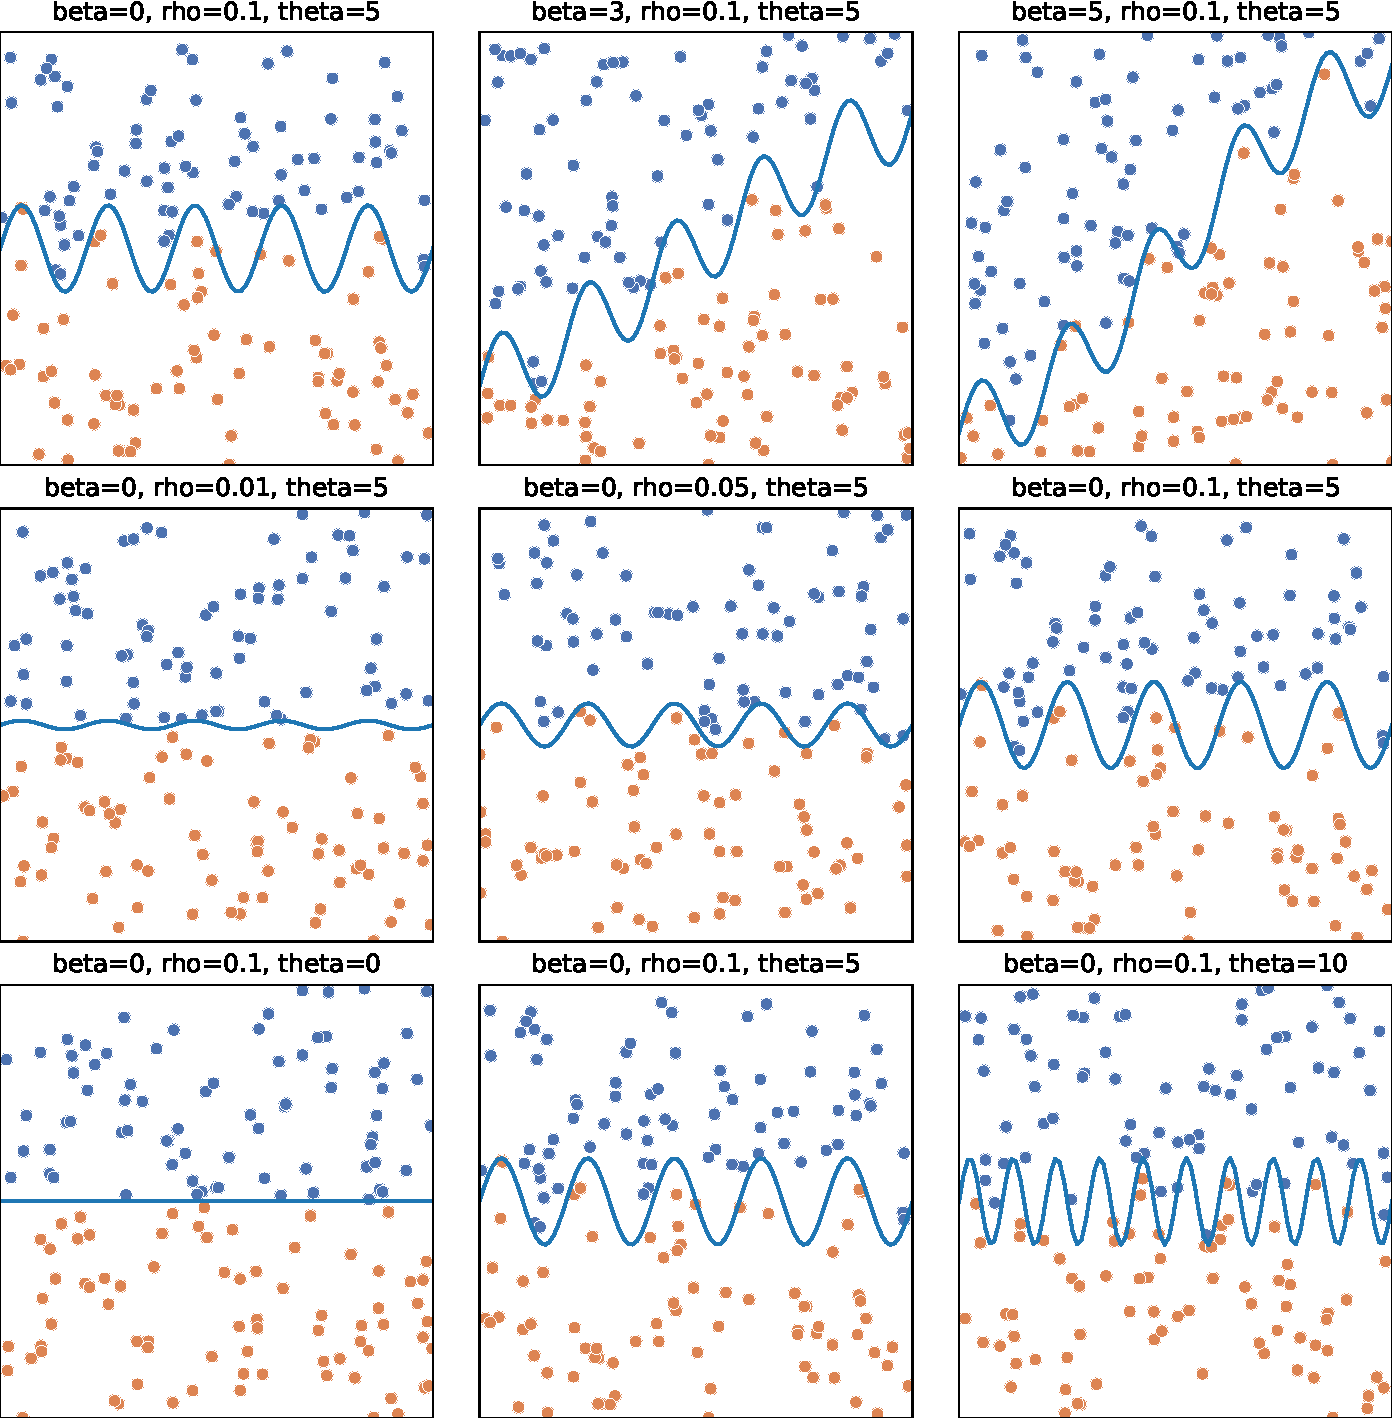
\includegraphics[width=\linewidth]{img/sinusoid_dataset_param_influence.pdf}
    \caption[Esempio di \emph{dataset} sintetici generati con funzione sinusoidale.]{Esempio di \emph{dataset} sintetici generati con funzione sinusoidale. 
    $\beta$ controlla l'inclinazione, $\rho$ controlla l'ampiezza e $\theta$ la frequenza della curva utilizzata per etichettare i vettori bidimensionali.}
    \label{fig:sinusoid_dataset}
\end{figure}
\begin{figure}
    \centering
    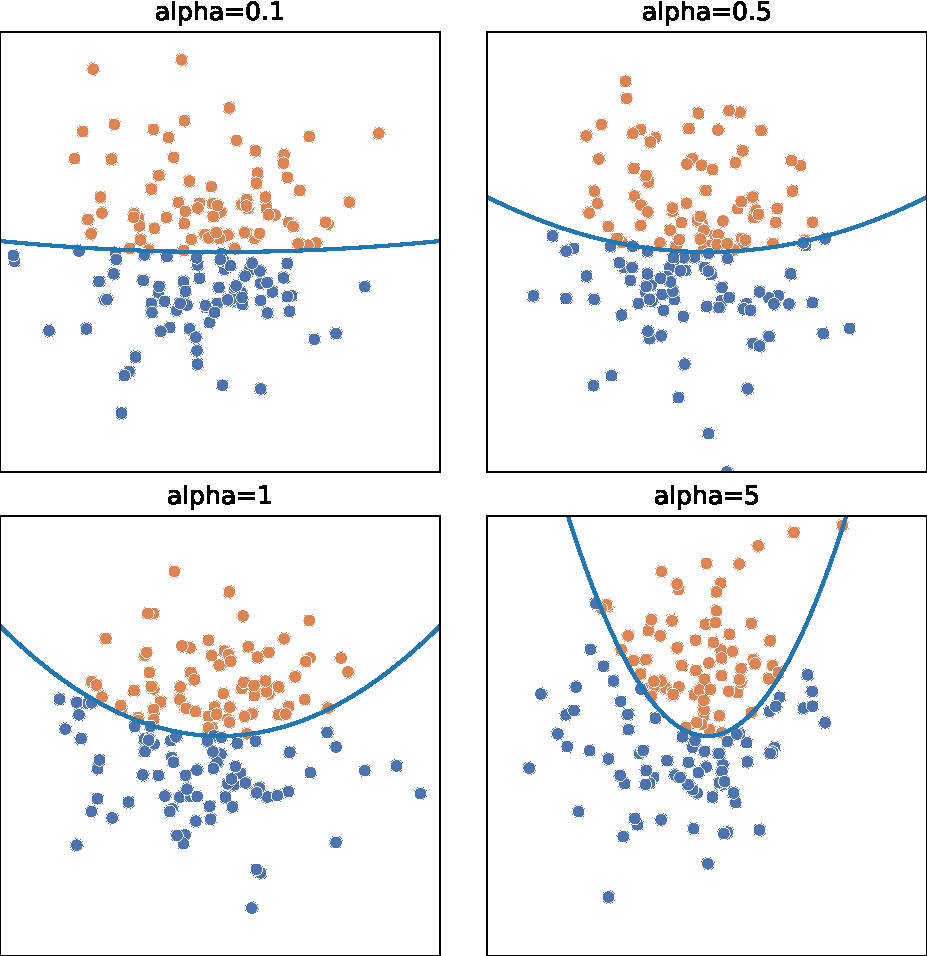
\includegraphics[width=.7\linewidth]{img/pacman_dataset_param_influence.pdf}
    \caption[Esempio di \emph{dataset} sintetici generati con funzione paraboloide.]{Esempio di \emph{dataset} sintetici generati con funzione paraboloide. Il parametro $\alpha$ controlla l'ampiezza della funzione di etichettamento.}
    \label{fig:pacman_dataset}
\end{figure}
A prescindere dalla funzione di etichettatura utilizzata, la procedura di generazione del \emph{dataset} è descritta nell'\Cref{alg:generazione_dataset_sintetici}.
Questa procedura richiede diversi parametri, descritti nell'elenco seguente.
\begin{itemize}
    \item Il parametro $n$ che identifica la dimensione totale del \emph{dataset}.
    \item Il parametri $d$ che identifica la dimensionalità dei punti del \emph{dataset} (quando si utilizza la funzione paraboloide). 
    \item Il parametro \emph{seed} o seme, utilizzato per il generatore di numeri casuali.
    \item Il parametro \emph{test\_size} è la percentuale di $n$ da riservare come insieme di \emph{test}.
    \item Il parametro 
    \begin{equation*}
        p = \frac{\text{numero di elementi con etichetta positiva}}{\text{numero di elementi con etichetta negativa}}
    \end{equation*} 
    regola il bilanciamento tra le classi.
    \item Il parametro $r$ regola il grado di rumore nei dati: indica la percentuale di elementi della classe positiva e altrettanti esempi della classe negativa da selezionare a caso per poi invertirne l'etichetta.
\end{itemize}
\begin{algorithm}
    \SetAlgoLined
    \KwData{
        $n>0 \in \mathrm{N}$ dimensione del \emph{dataset} desiderata\\ 
        $d>0 \in \mathrm{N}$ numero di attributi di ogni elemento (quando si utilizza la funzione paraboloide) \\
        $p \in [0,1]$ per regolare il bilanciamento tra classi\\
        $r \in [0,1]$ per regolare la quantità di rumore\\
        \emph{test\_size} percentuale di dati da ritornare come \emph{test set}\\
        $s$ seme per inizializzare il generatore di numeri pseudocasuali\\
    }
    \KwResult{Una matrice $X$ contenente $n$ vettori e un vettore $y$ contenente $n$ etichette, suddivisi in addestramento e \emph{test}}
    Inizializza il generatore casuale utilizzando il seme $s$\;
    $X_{\text{pop}} \gets$ seleziona a caso $10n$ elementi uniformemente a caso\;
    $y_{\text{pop}} \gets$ etichette dei vettori $X_{\text{pop}}$\;
    %
    $N_p \gets \lfloor\frac{n}{p + 1}\rfloor$\;
    $N_n \gets n - N_p$\;
    $X, y \gets$ seleziona da $X_{\text{pop}}$ uniformemente a caso $N_p$ elementi con le rispettive etichette positiva e seleziona da $X_{\text{pop}}$ uniformemente a caso $N_p$ elementi con le rispettive etichette negative\;
    seleziona a caso $\lfloor rN_p \rfloor$\ esempi della classe positiva e $\lfloor r  N_n \rfloor$\ elementi della classe negativa e inverti le loro etichette\;
    $X_{\text{test}}, y_{\text{test}} \gets$ seleziona \emph{test\_size} elementi (con rispettive etichette) a caso come test set\;
    $X_{\text{train}} \gets X \setminus X_{\text{test}}$\;
    $y_{\text{train}} \gets y \setminus y_{\text{test}}$\;
    Ritorna $X_{\text{train}}, X_{\text{test}}, y_{\text{train}}, y_{\text{test}}$\;
\caption{Procedura per la generazione di \emph{dataset} sintetico.}
\label{alg:generazione_dataset_sintetici}
\end{algorithm}

% \subsubsection{Funzione sinusoidale}
% Fissando i parametri $\beta,\rho,\theta$, per un vettore $\Vec{x}=\{x_1,x_2\}$, l'etichetta $y$ è calcolata con la funzione
% \begin{equation}\label{eq:sinusoid_dataset_lf}
% lf(\Vec{x}) = \sign\left(\frac{1}{(1 + \exp(-\beta(x_1 - 0.5)) + \rho \sin(2\pi\theta x_1)} - x2\right).
% \end{equation}
% Questa funzione di etichettatura è utilizzata solo per dati in spazi con due dimensioni. La~\cref{fig:sinusoid_dataset} mostra alcuni esempi di \emph{dataset} e funzioni di etichettatura al variare dei parametri.
% \begin{figure}
%     \centering
%     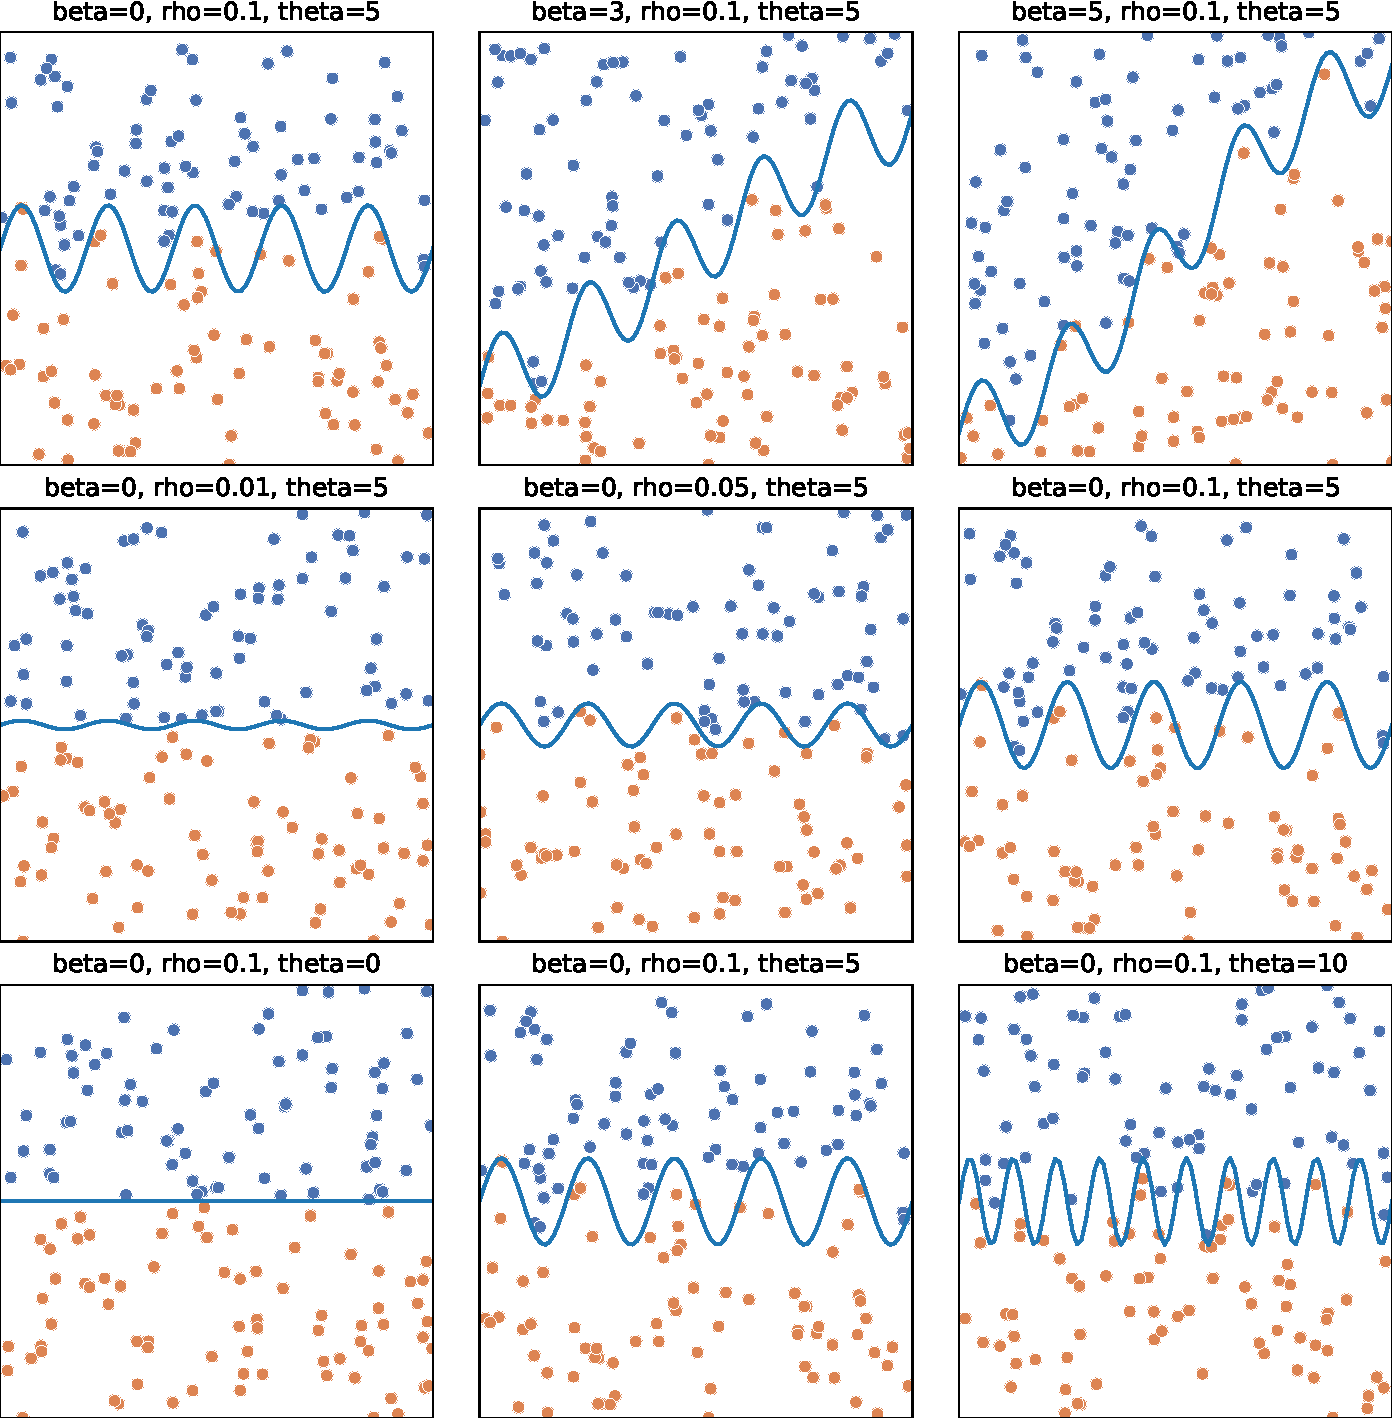
\includegraphics[width=1\linewidth]{img/sinusoid_dataset_param_influence.pdf}
%     \caption{Esempio di \emph{dataset} generati con funzione sinusoidale. 
%     $\beta$ controlla la pendenza, $\rho$ controlla l'ampiezza, $\theta$ la frequenza.}
%     \label{fig:sinusoid_dataset}
% \end{figure}
% \subsubsection{Funzione paraboloide}
% Fissati i parametri $\alpha, x_\text{shift}, y_\text{shift}$, per un vettore $\Vec{x}=\{x_1, \dots, x_n\} \in \mathrm{R}^n$, l'etichetta $y$ è calcolata con la funzione
% \begin{equation}\label{eq:pacman_dataset_lf}
% lf(\Vec{x})= x_n - \sum_{i=1}^{n-1}\alpha(x_i - x_\text{shift})^2 - y_\text{shift}.
% \end{equation}
% Il parametro $\alpha$ controlla l'ampiezza del paraboloide, mentre $x_\text{shift}$ e $y_\text{shift}$ traslano il vertice del paraboloide.
% La~\Cref{fig:pacman_dataset} mostra alcuni esempi di \emph{dataset} e funzioni di etichettatura al variare dei parametri.
% \begin{figure}
%     \centering
%     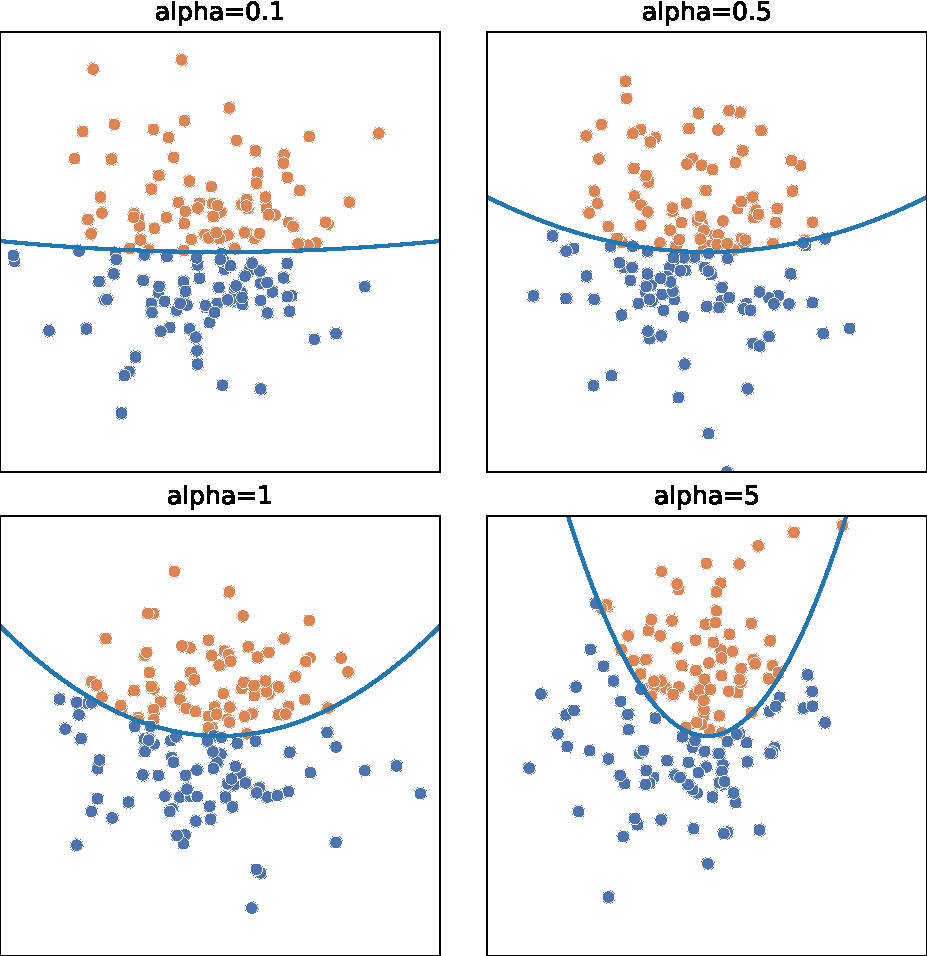
\includegraphics[width=1\linewidth]{img/pacman_dataset_param_influence.pdf}
%     \caption{Esempio di \emph{dataset} etichettati con paraboloide. Il parametro $\alpha$ controlla l'ampiezza.}
%     \label{fig:pacman_dataset}
% \end{figure}
I parametri per le funzioni di etichettatura utilizzati per la generazione dei \emph{dataset} sono scelti in modo da avere vari livelli di difficoltà di classificazione, misurata con le metriche esposte in~\Cref{sec:metriche_dataset}.
La difficoltà può essere gradualmente aumentata per esempio stringendo progressivamente il paraboloide o aumentando la frequenza o l'ampiezza della funzione sinusoidale.

La procedura nell'\Cref{alg:generazione_dataset_sintetici} utilizza delle estrazioni casuali in diversi punti:
\begin{itemize}
    \item per selezionare la popolazione iniziale;
    \item per estrarre i dati di test;
    \item eventualmente nella procedura di introduzione del rumore, per selezionare gli esempi a cui invertire l'etichetta.
\end{itemize}

\subsection{Dataset di terze parti}
I \emph{dataset} di terze parti utilizzati per alcuni esperimenti provengono dalla pagina web della libreria LibSVM\footnote{\url{https://www.csie.ntu.edu.tw/~cjlin/libsvmtools/datasets/binary.html}}.
Sono \emph{dataset} utilizzati in letteratura ma pre-elaborati (scalando e normalizzando gli attributi) e resi disponibili in formato LibSVM~\cite{libsvm}.
Si riportano in~\Cref{tab:uci_datasets} le caratteristiche dei \emph{dataset} utilizzati.
\begin{table}
    \centering
    \begin{tabular}{cccc}
        \toprule
        Nome & Num. dati addestramento & Num. dati \emph{test} & Num. attributi\\
        \midrule
        svmguide1 &  3,089 & 4,000 & 4 \\
        a1a & 1,605	& 30,956 & 123\\
        gisette & 6000 & 1000 & 5000 \\
        \bottomrule
    \end{tabular}
    \caption{Caratteristiche dei \emph{dataset} di terze parti.}
    \label{tab:uci_datasets}
\end{table}


\section{Impostazione degli esperimenti}\label{sec:impostazione_esperimenti}
A prescindere dai \emph{dataset} utilizzati, la maggior parte degli esperimenti ha delle caratteristiche in comune:
\begin{itemize}
    \item la strategia utilizzata per definire le riduzioni di \emph{budget};
    \item il metodo di valutazione e selezione dei modelli;
    \item l'ambiente di esecuzione.
\end{itemize}
Questi aspetti sono discussi nei prossimi paragrafi.

\subsection{Strategia 1}
Il procedimento è descritto di seguito. Per prima cosa si addestra un modello SVM tradizionale senza nessun vincolo sul numero di vettori di supporto. Chiamiamo questo modello $FM$ e chiamiamo $FB$ il numero di vettori di supporto di $FM$.
In seguito, si addestrano una serie di modelli con un \emph{budget} pari a una frazione di $FB$.
Per ognuno di questi modelli il \emph{budget} è espresso come $B=pFM$, dove
\begin{equation*}
    p\in\{0.3, 0.4, 0.5, 0.6, 0.7, 0.8, 0.9\}.
\end{equation*}
Nei grafici dei risultati ottenuti con questa strategia compare anche il valore di \emph{budget} che corrisponde a $p=1$: indica dei modelli classici senza nessun vincolo di \emph{budget}.
Nell'\Cref{alg:esperimenti_1} è descritto lo pseudocodice per la strategia.
\begin{algorithm}
    \SetAlgoLined
    \KwData{\emph{dataset} da analizzare}
    %\KwResult{}
    $FM \gets$ seleziona il miglior modello senza imporre nessun vincolo di \emph{budget}\;
    $FB \gets$ numero di vettori di supporto del modello $FM$\;
    salva parametri e dettagli di $FM$\;
    \For{$p\gets0.3$ \KwTo $0.9$ \KwBy $0.1$}{
        $B\gets pFB$\;
        $M \gets$ seleziona il miglior modello con $\text{budget}=B$\;
        salva parametri e dettagli di $M$\;
    }
\caption{Pseudocodice strategia 1.}
\label{alg:esperimenti_1}
\end{algorithm}

Utilizzando questa strategia è possibile misurare l'accuratezza sui dati di \emph{test} al diminuire del \emph{budget} e paragonarla all'accuratezza del corrispettivo modello classico addestrato sullo stesso dataset.
Per ogni modello, si definisce \emph{score ratio} la quantità
\begin{equation*}
    \text{score ratio} = \frac{\text{accuratezza su dati di \emph{test} del modello \emph{budgeted SVC}}}{\text{accuratezza su dati di \emph{test} del corrispettivo modello classico}}.
\end{equation*}

Con questi esperimenti è possibile ottenere delle indicazioni su quanto sia possibile ridurre il \emph{budget} senza penalizzare troppo l'accuratezza, limitatamente ai \emph{dataset} considerati e in rapporto alla controparte senza vincolo sul \emph{budget}.

Per mitigare un eventuale \emph{bias} dovuto alla casualità nella generazione del dataset, si è deciso in alcuni casi di generare tre \emph{dataset} per ogni gruppo di parametri utilizzando altrettanti valori del parametro seme.
La procedura completa, in questo caso, è descritta nell'~\Cref{alg:esperimenti_2}.
\begin{algorithm}
    \SetAlgoLined
    \KwData{\emph{parametri\_dataset} $\gets$ le varie combinazioni di parametri per generare dataset.}    
    \For{$s \gets \text{estrai nuovo seme}$}{
        \For{params \KwIn \emph{parametri\_dataset}}{
            $ds\gets$ genera \emph{dataset} con l'\Cref{alg:generazione_dataset_sintetici} usando $params$ e $s$\;
            esegui l'\Cref{alg:esperimenti_1} su $ds$\;           
        }
    }
\caption{Pseudocodice esperimenti con strategia 1 e con ripetizione della generazione dei dataset.}
\label{alg:esperimenti_2}
\end{algorithm}

\subsection{Strategia 2}
Un secondo approccio per eseguire gli esperimenti su un certo \emph{dataset} consiste nell'esprimere il \emph{budget} in funzione della dimensione del \emph{dataset} invece che in funzione del numero di vettori di supporto di un modello classico.
Questa strategia è descritta nell'\Cref{alg:esperimenti_3}.
\begin{algorithm}
    \SetAlgoLined
    \KwData{\emph{dataset}}
    %\KwResult{}
    $m \gets |\textit{dataset}|$\;
    \For{$p$ \KwIn $\{0.01, 0.025, 0.05, 0.075, 0.1, 0.125, 0.15, 0.175, 0.2\}$}{
        $B\gets pm$\;
        $M \gets$ seleziona il miglior modello con \emph{budget} $B$ su \emph{dataset}\;
        salva parametri e dettagli di $M$\;
    }
\caption{Pseudocodice strategia 2.}
\label{alg:esperimenti_3}
\end{algorithm}
Per un certo \emph{dataset} composto da $m$ elementi, si esprime il \emph{budget} come $B=pm$, dove
\begin{equation*}
    p\in\{0.01, 0.025, 0.05, 0.075, 0.1, 0.125, 0.15, 0.175, 0.2\}.
\end{equation*}
Così facendo è possibile verificare la bontà dei modelli con un \emph{budget} molto stringente, fino all'$1\%$ dei dati di addestramento.

Per gli esperimenti effettuati con questa strategia, i \emph{dataset} sintetici sono stati generati una sola volta con un solo seme per ogni configurazione di parametri.

\subsection{Selezione e valutazione dei modelli}
Ogni modello è valutato sullo stesso insieme di dati di \emph{test} per ogni \emph{dataset}.
Nel caso dei dati di terze parti, l'insieme di \emph{test} è già fornito, mentre nel caso di dati sintetici l'insieme di \emph{test} viene selezionato dopo la procedura di generazione e non viene più modificato.
L'insieme di \emph{test} è scelto casualmente, ma mantiene il bilanciamento delle classi dei dati di addestramento.

I migliori iperparametri sono selezionati sui dati di addestramento utilizzando \emph{5-fold cross validation}, con una ricerca esaustiva sulla griglia di parametri descritta in~\Cref{tab:gridsearch_2d}.
\begin{table}
    \centering
    \begin{tabular}{cccc}
        \toprule
        $C$ & \emph{Kernel} & $\gamma$ & d \\
        \midrule
        \multirow{3}{*}{[0.01, 0.1, 1, 10]} & Gaussiano   & [0.0001, 0.001, 0.01, 0.1, 1, 10]   & /\\
                                            \cline{2-4}
                                            & Polinomiale   & / & [2, 5, 10] \\
                                            \cline{2-4}
                                            & Lineare       & / & / \\
        \bottomrule
    \end{tabular}
    \caption{Griglia di iperparametri per selezionare i modelli \emph{budgeted SVC}.}
    \label{tab:gridsearch_2d}
\end{table}
Questi parametri sono riferiti al metodo \emph{budgeted SVC}; nel caso in cui un esperimento sia stato eseguito con una griglia differente, sarà specificato nel paragrafo che lo descrive.

\subsection{Ambiente di esecuzione}
Tutti gli esperimenti sono stati eseguiti su un server con CPU Intel(R) Xeon(R) W-1250P CPU @ 4.10GHz e con 31GB di ram. Il linguaggio di programmazione utilizzato è Python 3.10.10. \`E stato utilizzato il risolutore Gurobi 10.0.1~\cite{gurobi} per risolvere i problemi di ottimizzazione sia dei modelli SVC classici che \emph{budgeted SVC}.

Per cercare di ridurre il carico computazionale, gli esperimenti effettuati utilizzando la formulazione \emph{budgeted SVC} utilizzano una matrice \emph{kernel} pre-calcolata; le implementazioni di altri metodi presenti in letteratura utilizzati come confronto, invece, calcolano i valori di \emph{kernel} durante l'addestramento.

Il limite massimo di tempo concesso al risolutore per risolvere ogni istanza del problema di ottimizzazione è di sessanta secondi.

\section{Esperimenti su dataset sintetici 2D}\label{sec:exp:synth_2d}
Si riportano in questo paragrafo i risultati degli esperimenti effettuati sui \emph{dataset} sintetici generati con le configurazioni di parametri riportate nelle~\Cref{tab:parametri_ds_sin,tab:parametri_ds_pacman}.
\begin{table}
    \centering
    \begin{tabular}{ccccc}
        \toprule
         $n$ & \emph{test\_size} & $\beta$ & $\rho$ & $\theta$ \\
        \midrule
        \multirow{10}{*}{1000} & \multirow{10}{*}{0.3} &\multirow{5}{*}{0}  & 0.01  & \multirow{5}{*}{20} \\        
                            &&& 0.025 &     \\        
                            &&& 0.05  &     \\        
                            &&& 0.075 &     \\        
                            &&& 0.1   &     \\
        \cline{3-5}
                &&  95      & 0.2   & 10    \\   
        \cline{3-5}
        &&  \multirow{4}{*}{0}  & \multirow{4}{*}{0.1}  & 1     \\    
                            &&&                       & 2     \\    
                            &&&                       & 5     \\    
                            &&&                       & 1     \\    
        \bottomrule
    \end{tabular}
    \caption{Configurazioni di parametri utilizzati per generare \emph{dataset} bidimensionali con la funzione sinusoidale (\ref{eq:sinusoid_dataset_lf}).}
    \label{tab:parametri_ds_sin}
\end{table}
\begin{table}
    \centering
    \begin{tabular}{ccccc}
        \toprule
         $n$ & \emph{test\_size} &$\alpha$ & $x_\text{shift}$ & $y_\text{shift}$ \\
        \midrule
        \multirow{5}{*}{1000} & \multirow{5}{*}{0.3} &1   & \multirow{5}{*}{0.5} & \multirow{5}{*}{0.5} \\
        && 2.5 &\\
        && 5   &\\
        && 7.5 &\\
        && 10  &\\
        \bottomrule
    \end{tabular}
    \caption{Configurazioni di parametri utilizzati per generare \emph{dataset} bidimensionali con la funzione parabola (\ref{eq:pacman_dataset_lf}).}
    \label{tab:parametri_ds_pacman}
\end{table}

\subsubsection{Esperimenti utilizzando la strategia 1}
La~\Cref{fig:risultati_2d} mostra dei grafici che riportano l'andamento dell'accuratezza e dello \emph{score ratio} ottenuti sui dati di \emph{test} al variare del \emph{budget}.
Questa figura mostra solo i risultati più significativi; i grafici omessi sono riportati nell'Appendice A.

Dai risultati ottenuti è possibile notare come per \emph{dataset} semplici, o con una funzione di etichettatura sinusoidale con tante oscillazioni ma ben approssimabile da una funzione lineare, il metodo proposto risulta efficace, portando a una riduzione significativa del numero di vettori di supporto senza pagare troppo in termini di accuratezza.
In altri casi, invece, con \emph{dataset} più difficili, il comportamento è diverso:
\begin{itemize}
    \item per piccole riduzioni di \emph{budget}, come $80\%$ e $90\%$ del numero di vettori di supporto del modello tradizionale, la perdita in accuratezza è moderata;
    \item per valori di \emph{budget} intermedi nel range considerato, tra il $40\%$ e il $70\%$ la perdita di accuratezza è più grave e marcata;
    \item per valori di \emph{budget} piccoli, come $30\%$ o $40\%$, l'accuratezza è migliore di quella ottenuta per diminuzioni di \emph{budget} tra il $40\%$ e il $70\%$.
\end{itemize}
Sempre per i \emph{dataset} più difficili, si nota anche un'alta variabilità nei risultati ottenuti nel gruppo di \emph{dataset} generati con stessi parametri ma seme diverso, con alcune istanze che esibiscono accuratezza molto bassa.
Dalla~\Cref{fig:risultati_2d} è possibile notare come i modelli peggiori siano associati a un'istanza del problema \emph{budgeted SVC} non risolta all'ottimo, perché il risolutore ha raggiunto il limite massimo di tempo concesso e ha restituito una soluzione non ottimale.
L'interpretazione è quindi che per riduzioni di \emph{budget} intermedie, il risolutore faccia più fatica a modellare la funzione originale perché non può utilizzare abbastanza vettori di supporto, mentre per \emph{budget} più ristretti la soluzione del problema sia più semplice perché è possibile escludere più velocemente un maggior numero di soluzioni.

Nei casi in cui si riscontra alta variabilità (utilizzando la stesa riduzione di \emph{budget} sullo stesso gruppo di \emph{dataset}) si può notare come si ottengano anche modelli buoni, spesso costruiti con una soluzione ottima.
\begin{figure}
    \begin{subfigure}{.5\textwidth}
        \centering
        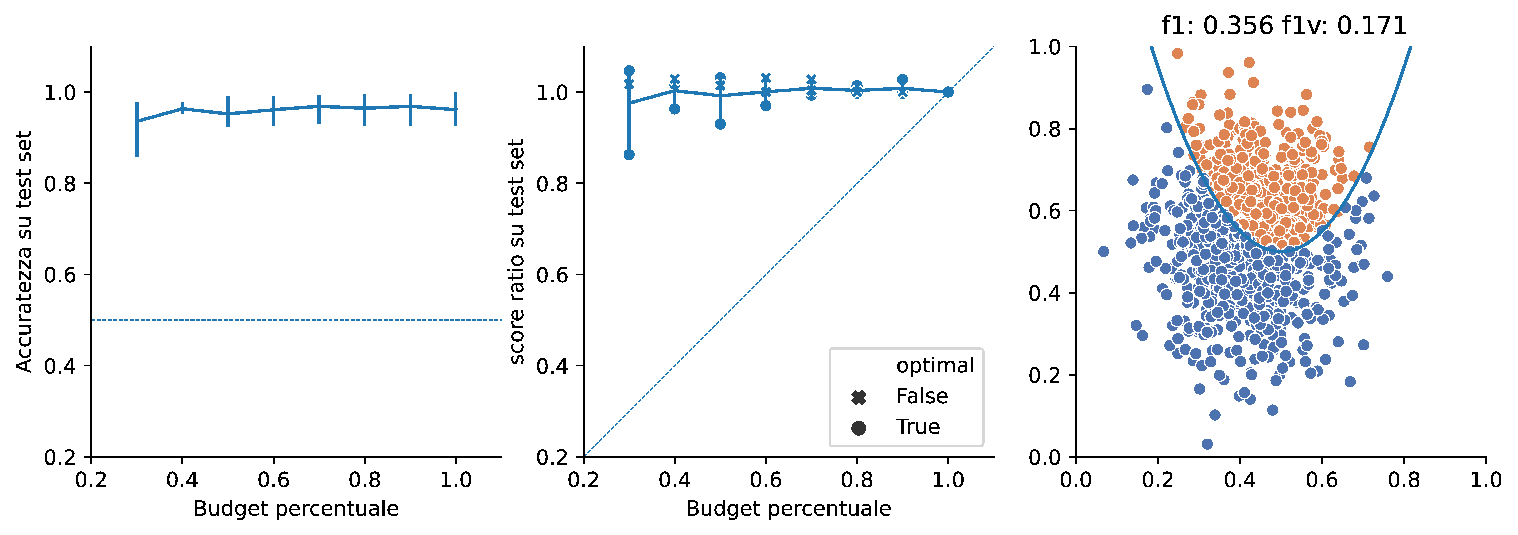
\includegraphics[width=\textwidth]{img/2d/3.pdf}
    \end{subfigure}%
    \begin{subfigure}{.5\textwidth}
        \centering
        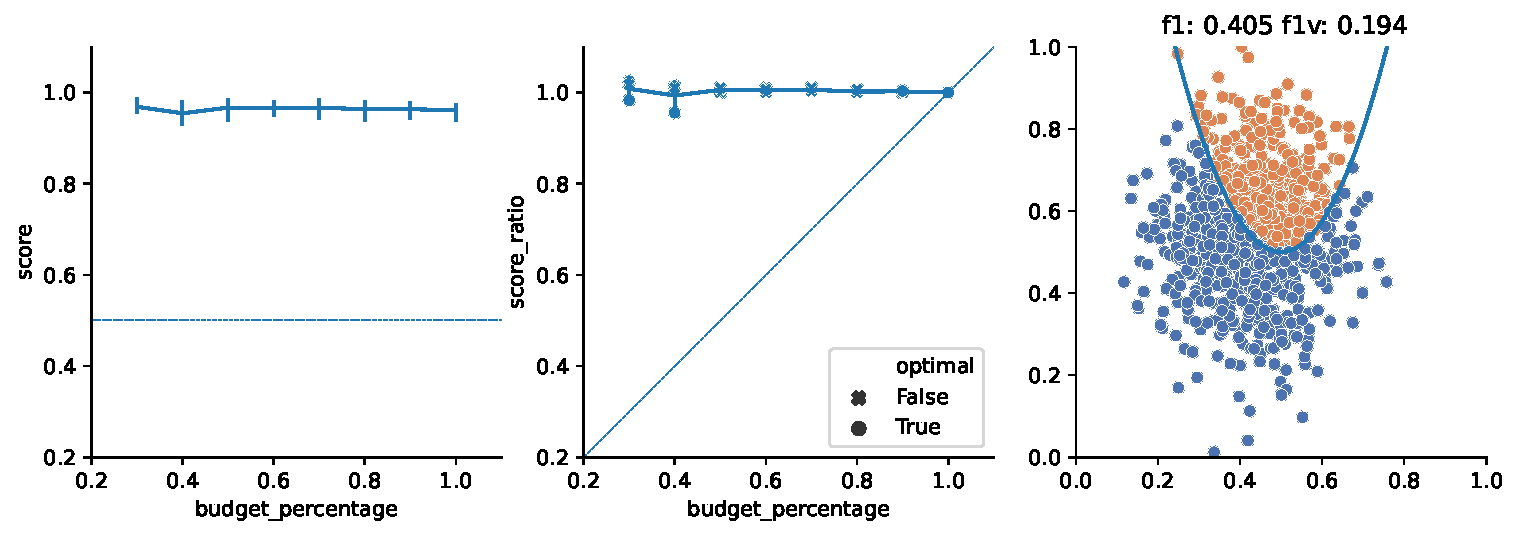
\includegraphics[width=\textwidth]{img/2d/4.pdf}
    \end{subfigure}%
    %
    \hfill
    %
    \begin{subfigure}{.5\textwidth}
        \centering
        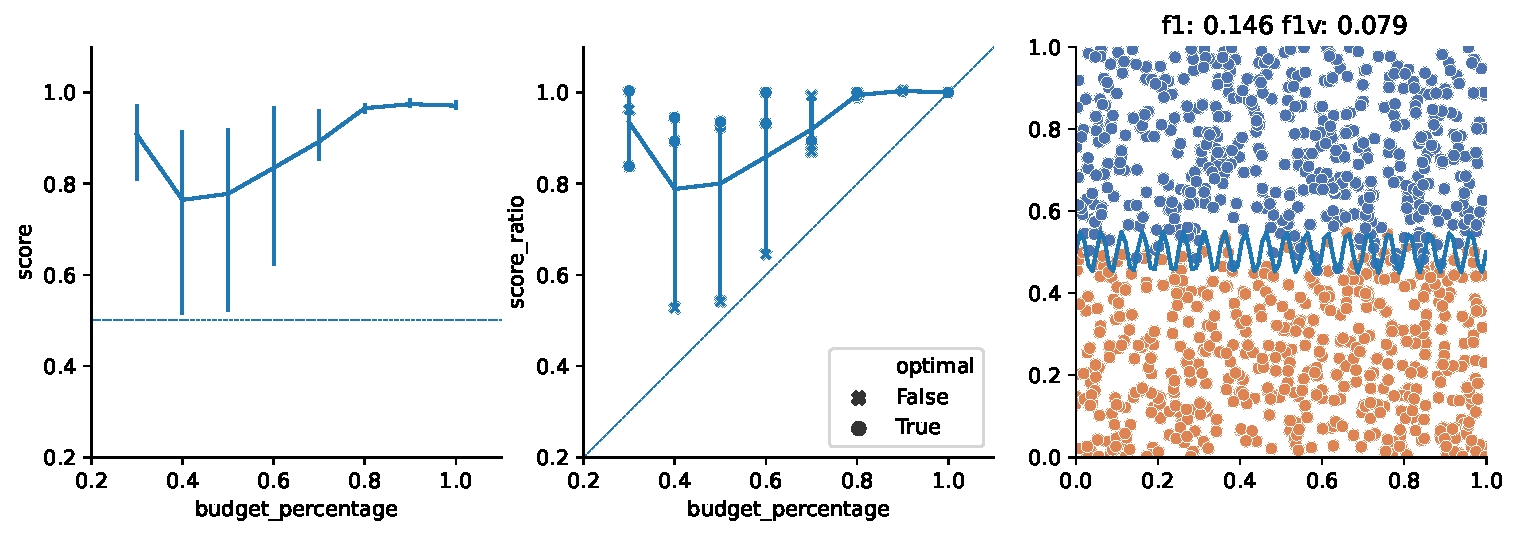
\includegraphics[width=\textwidth]{img/2d/8.pdf}
    \end{subfigure}%
    \begin{subfigure}{.5\textwidth}
        \centering
        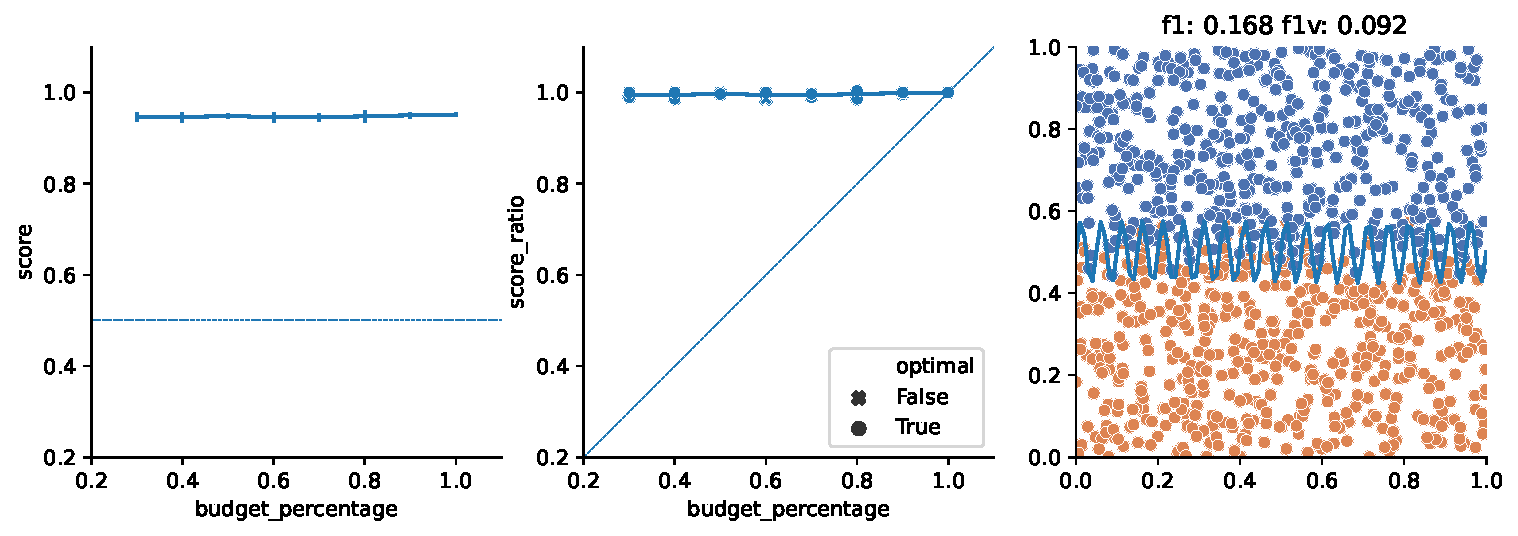
\includegraphics[width=\textwidth]{img/2d/9.pdf}
    \end{subfigure}%
    %
    \hfill
    %
    \begin{subfigure}{.5\textwidth}
        \centering
        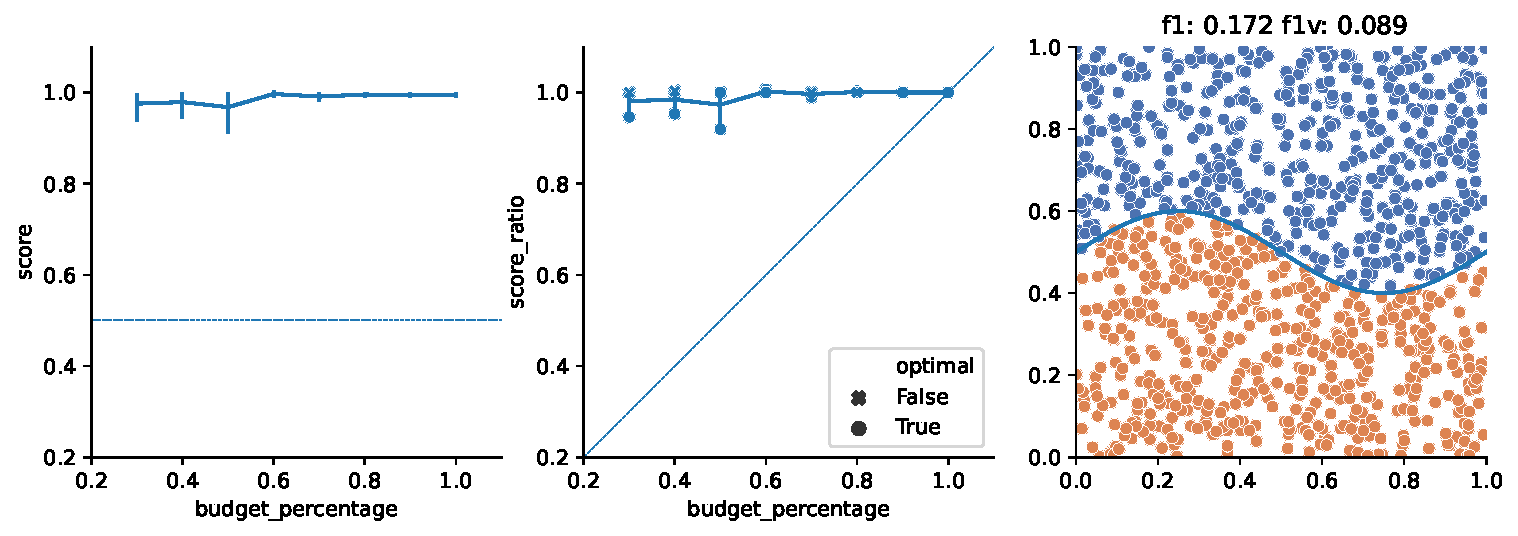
\includegraphics[width=\textwidth]{img/2d/10.pdf}
    \end{subfigure}%
    \begin{subfigure}{.5\textwidth}
        \centering
        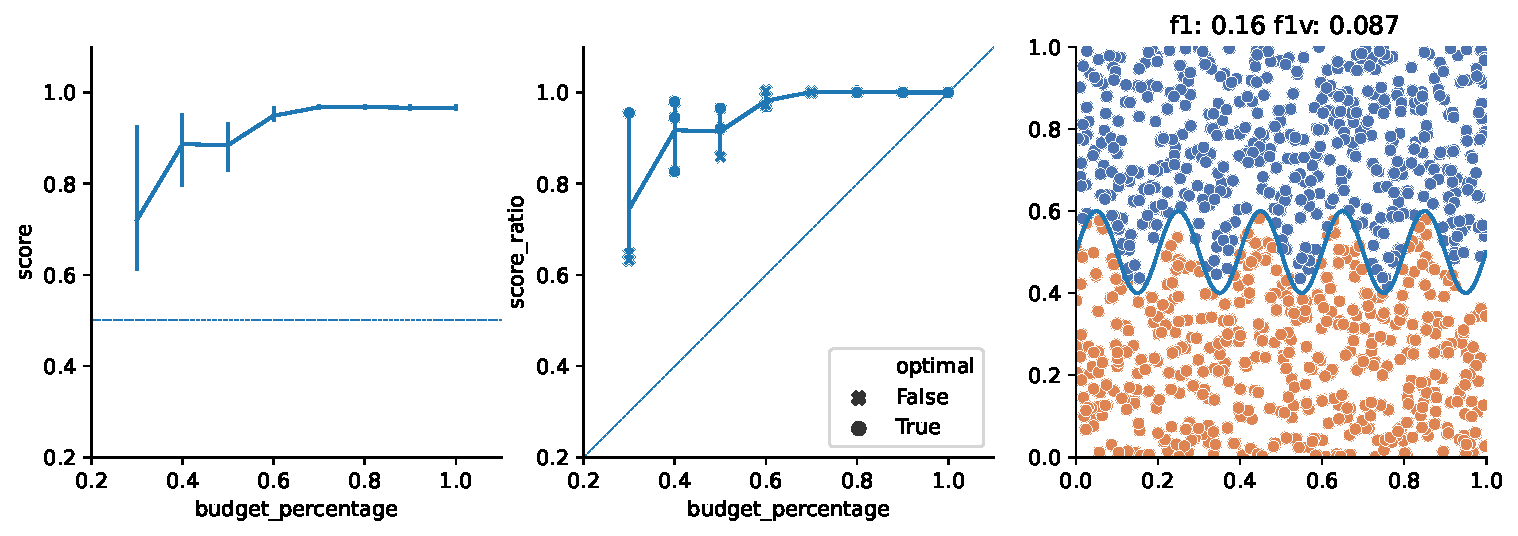
\includegraphics[width=\textwidth]{img/2d/12.pdf}
    \end{subfigure}%
     %
    \hfill
    %
    \begin{subfigure}{.5\textwidth}
        \centering
        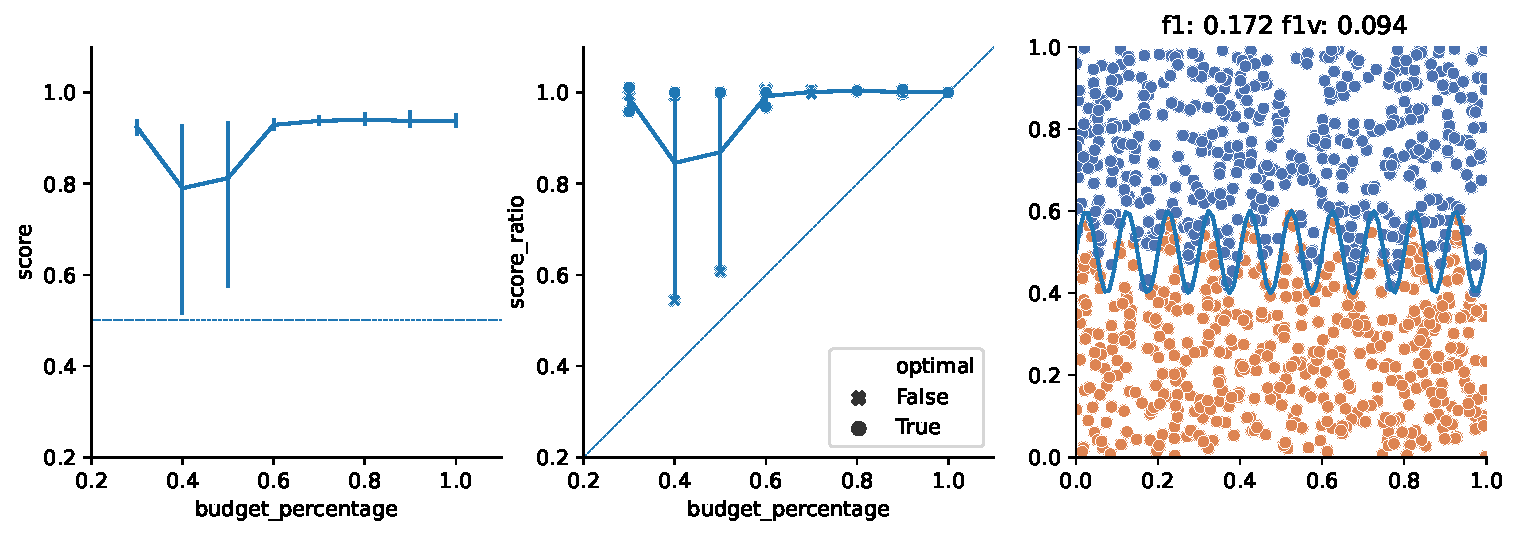
\includegraphics[width=\textwidth]{img/2d/13.pdf}
    \end{subfigure}%
    \begin{subfigure}{.5\textwidth}
        \centering
        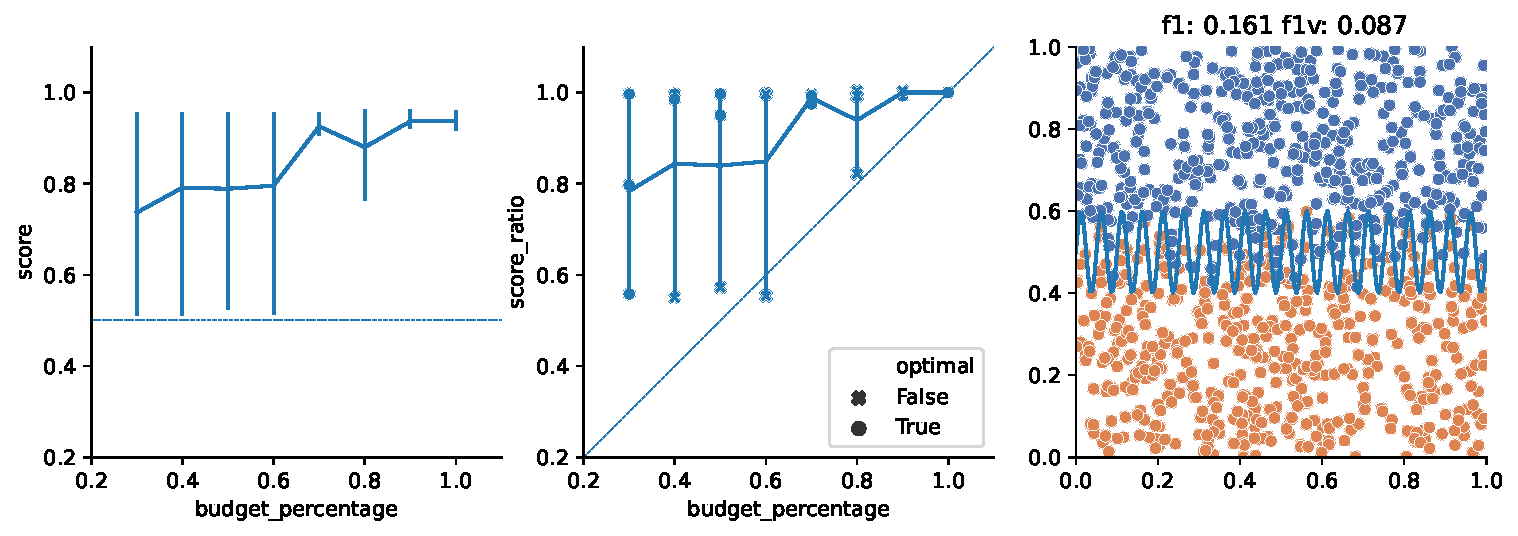
\includegraphics[width=\textwidth]{img/2d/14.pdf}
    \end{subfigure}%
     %
    \hfill
    %
    \begin{subfigure}{.5\textwidth}
        \centering
        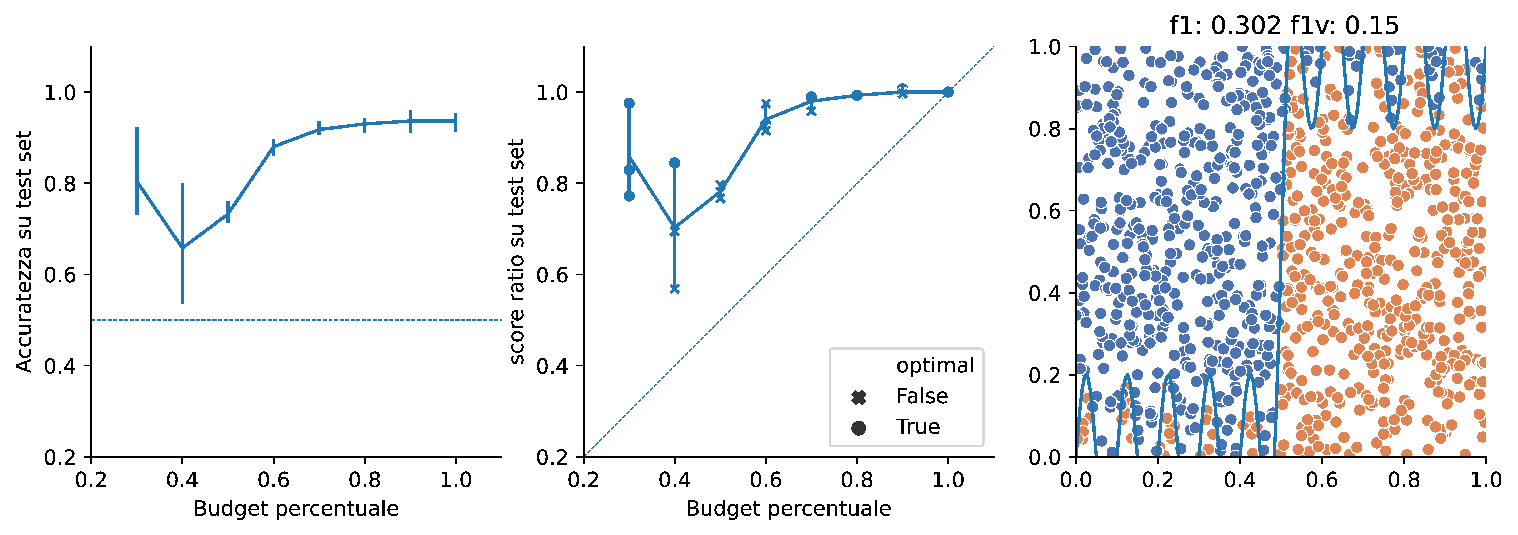
\includegraphics[width=\textwidth]{img/2d/15.pdf}
    \end{subfigure}%
    \caption[Risultati su \emph{dataset} sintetici utilizzando la strategia 1.]{Risultati più significativi ottenuti su \emph{dataset} sintetici 2D utilizzando la strategia 1. Ognuno dei grafici a sinistra indica l'andamento dell'accuratezza sui dati di \emph{test} al variare del \emph{budget}; ognuno dei grafici al centro indica lo \emph{score ratio} al variare del \emph{budget} (un simbolo ``x'' indica che il risolutore ha prodotto una soluzione non ottima); ognuno dei grafici a destra rappresenta uno dei tre \emph{dataset} utilizzati con le rispettive metriche di difficoltà.}
\label{fig:risultati_2d}
\end{figure}

% magari full_budget partiva già con "pochi" sv e ridurli porta ad accuracy molto più basse... ma non so

Analizzando il numero di vettori di supporto dei modelli tradizionali (vedi ~\Cref{fig:2d_dist_numsv}) è possibile notare come la maggior parte dei modelli abbia un numero ragionevole di vettori di supporto ma come una minoranza abbia invece un numero molto elevato.
\begin{figure}
    \centering
    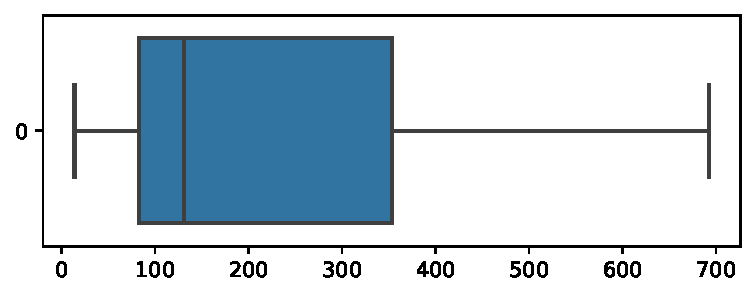
\includegraphics[width=0.5\linewidth]{img/2d/numsv.pdf}
    \caption{Distribuzione del numero di vettori di supporto per i modelli classici addestrati sui \emph{dataset} sintetici con la strategia 1.}
    \label{fig:2d_dist_numsv}
\end{figure}

\subsubsection{Risultati ottenuti utilizzando la strategia 2}
Utilizzando gli stessi \emph{dataset} dell'esperimento precedente, sono stati effettuati ulteriori esperimenti utilizzando la strategia 2.
In~\Cref{fig:2d_v2} si riporta l'andamento dell'accuratezza sui dati di \emph{test} al variare del \emph{budget} per ogni \emph{dataset}.
Questa figura mostra solo i risultati più significativi; i grafici omessi sono riportati nell'Appendice A.

\begin{figure}
    \begin{subfigure}{.5\textwidth}
        \centering
        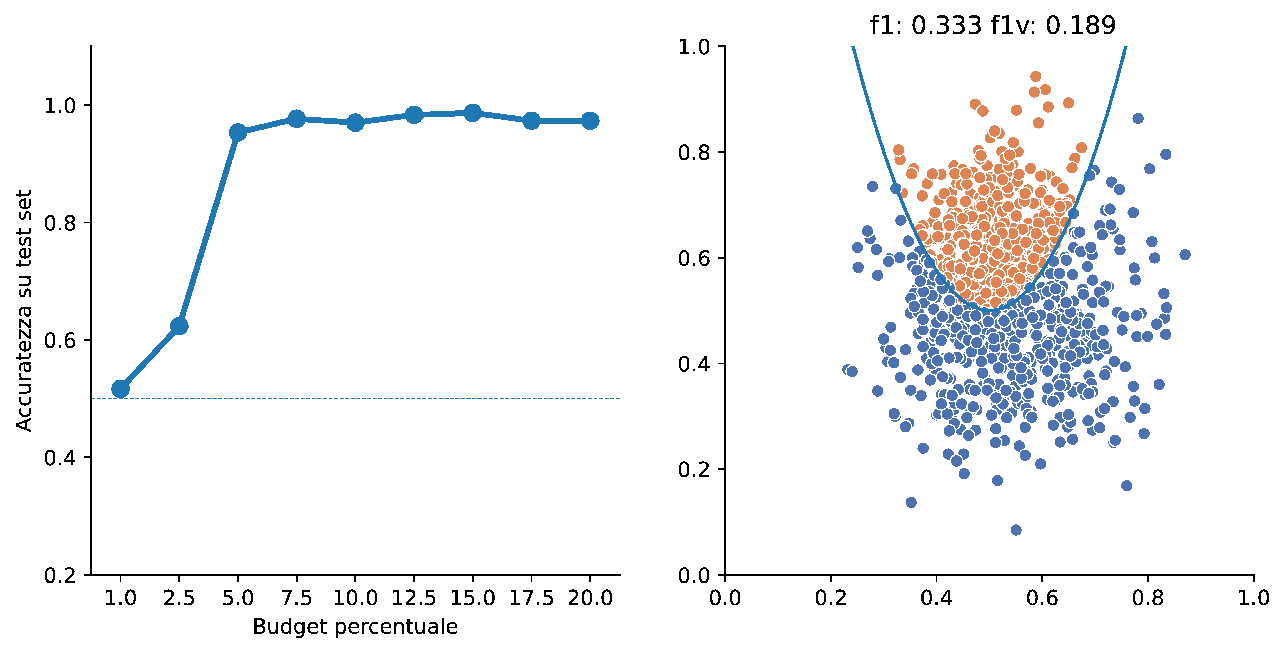
\includegraphics[width=\textwidth]{img/2d_v2/4.pdf}
    \end{subfigure}%
    \begin{subfigure}{.5\textwidth}
        \centering
        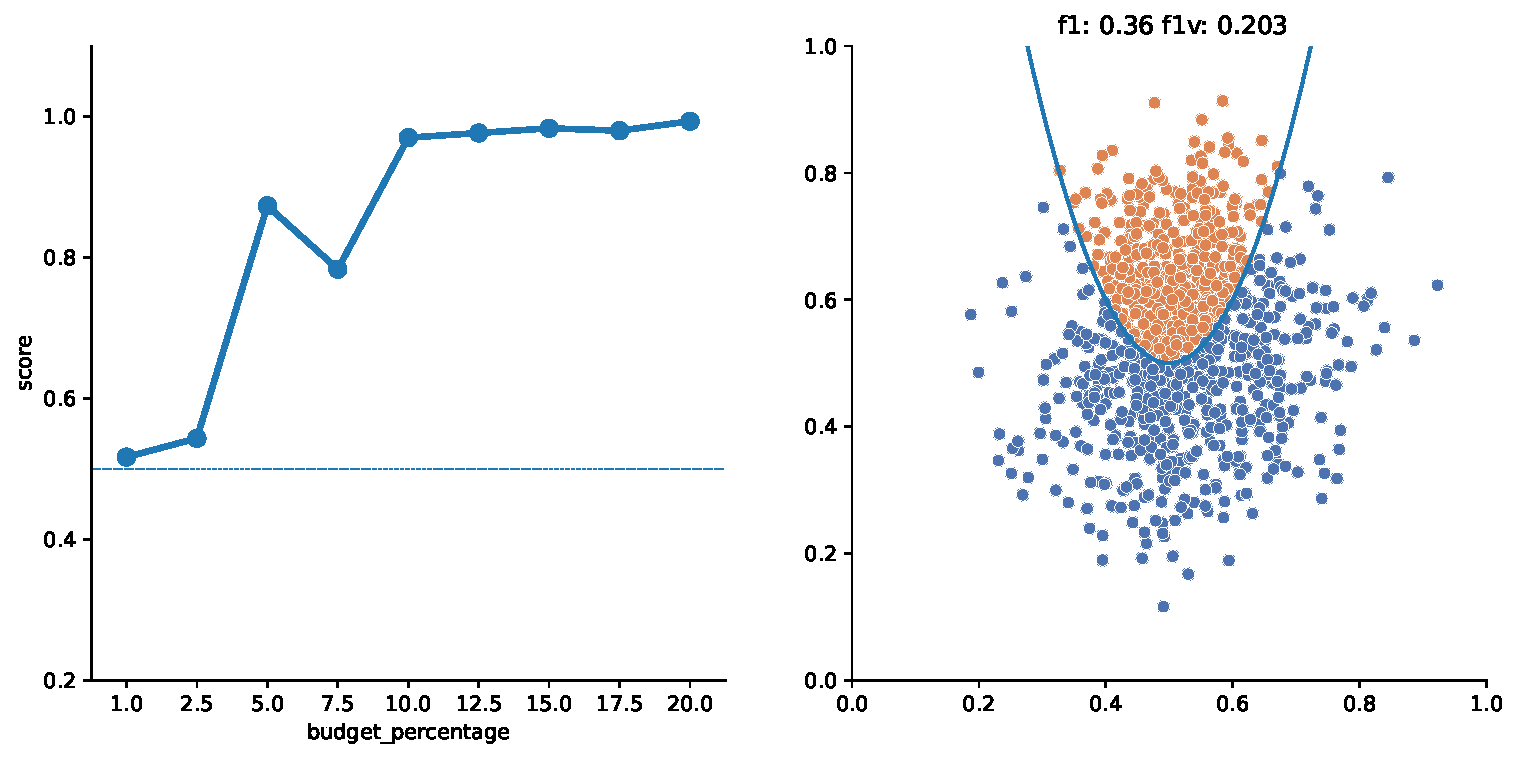
\includegraphics[width=\textwidth]{img/2d_v2/5.pdf}
    \end{subfigure}
    %
    \hfill
    %
    \begin{subfigure}{.5\textwidth}
        \centering
        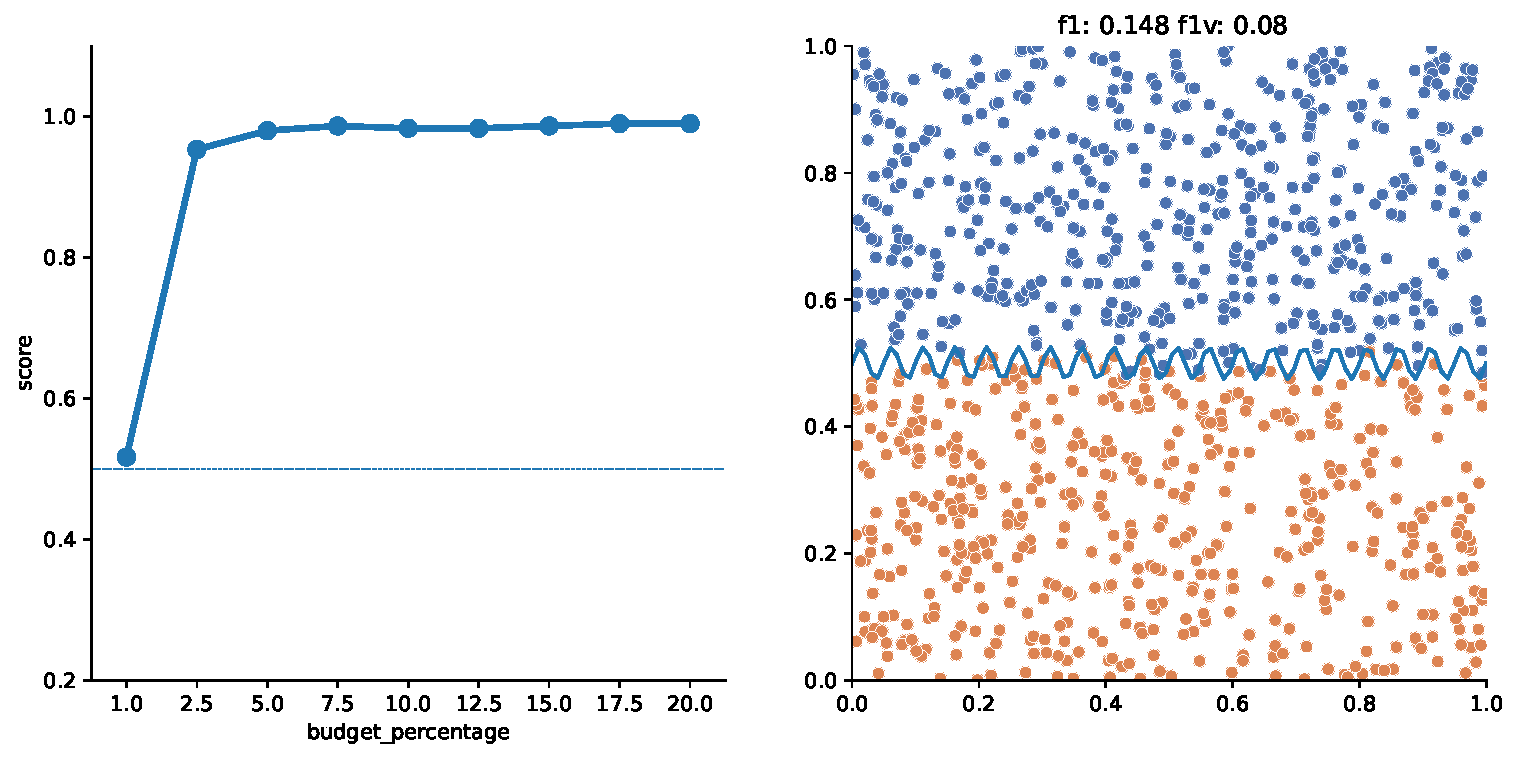
\includegraphics[width=\textwidth]{img/2d_v2/7.pdf}
    \end{subfigure}
    \begin{subfigure}{.5\textwidth}
        \centering
        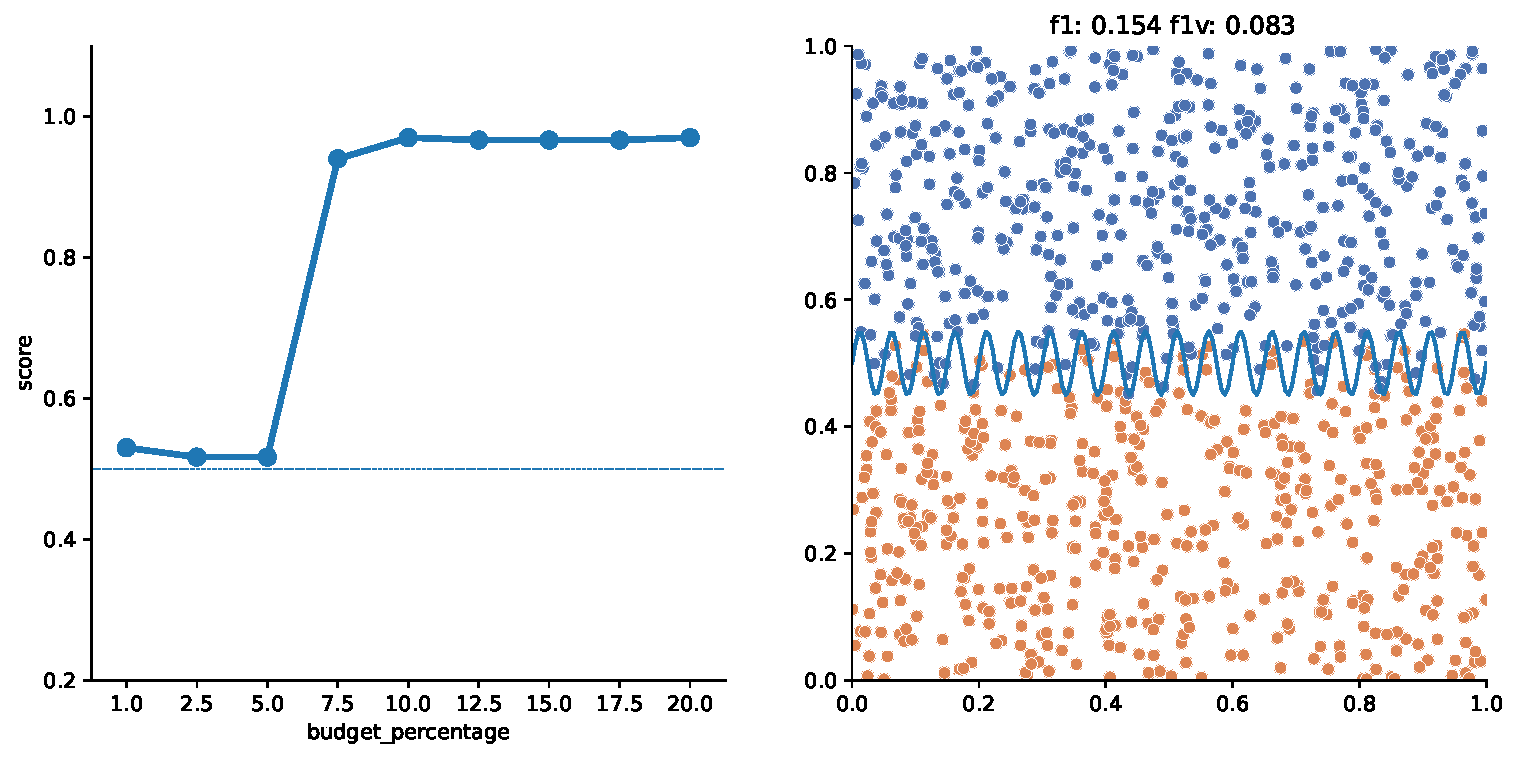
\includegraphics[width=\textwidth]{img/2d_v2/8.pdf}
    \end{subfigure}%
    %
    \hfill
    %
    \begin{subfigure}{.5\textwidth}
        \centering
        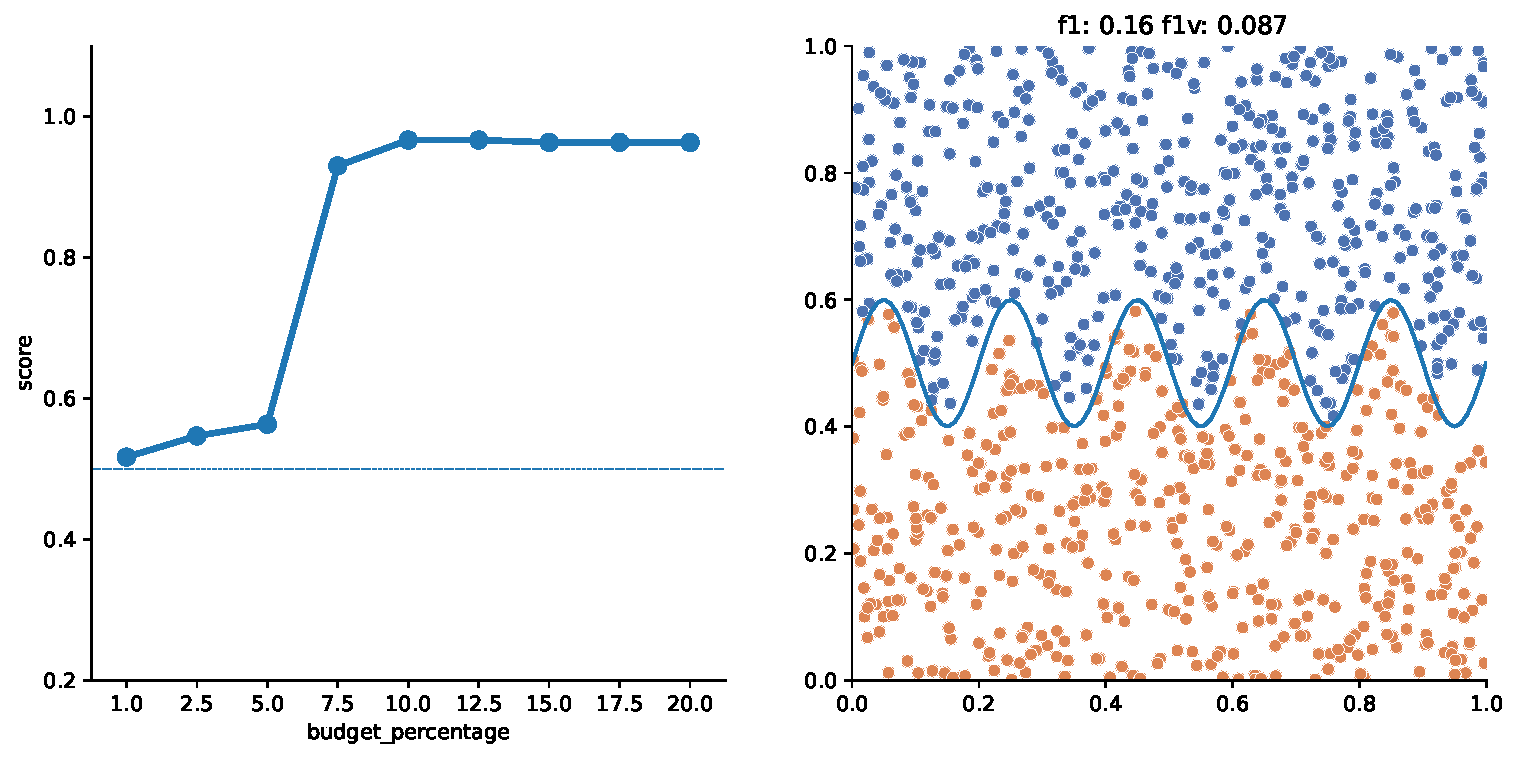
\includegraphics[width=\textwidth]{img/2d_v2/12.pdf}
    \end{subfigure}
    \begin{subfigure}{.5\textwidth}
        \centering
        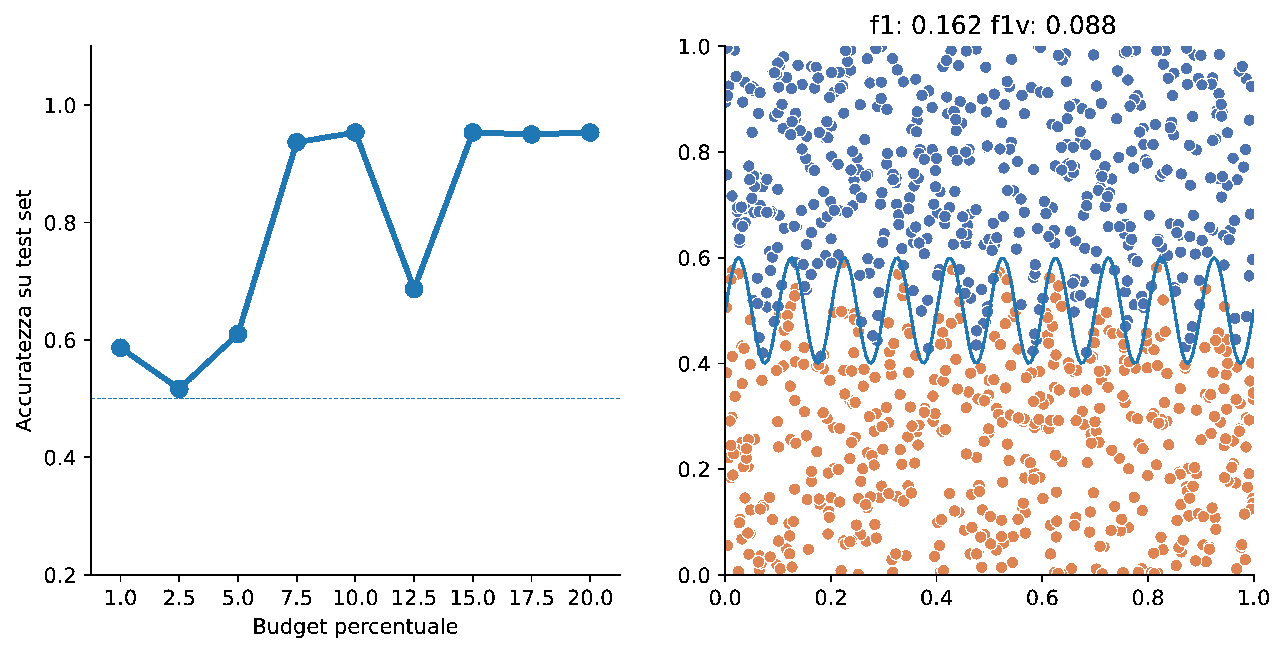
\includegraphics[width=\textwidth]{img/2d_v2/13.pdf}
    \end{subfigure}%
    %
    \hfill
    %
    \begin{subfigure}{.5\textwidth}
        \centering
        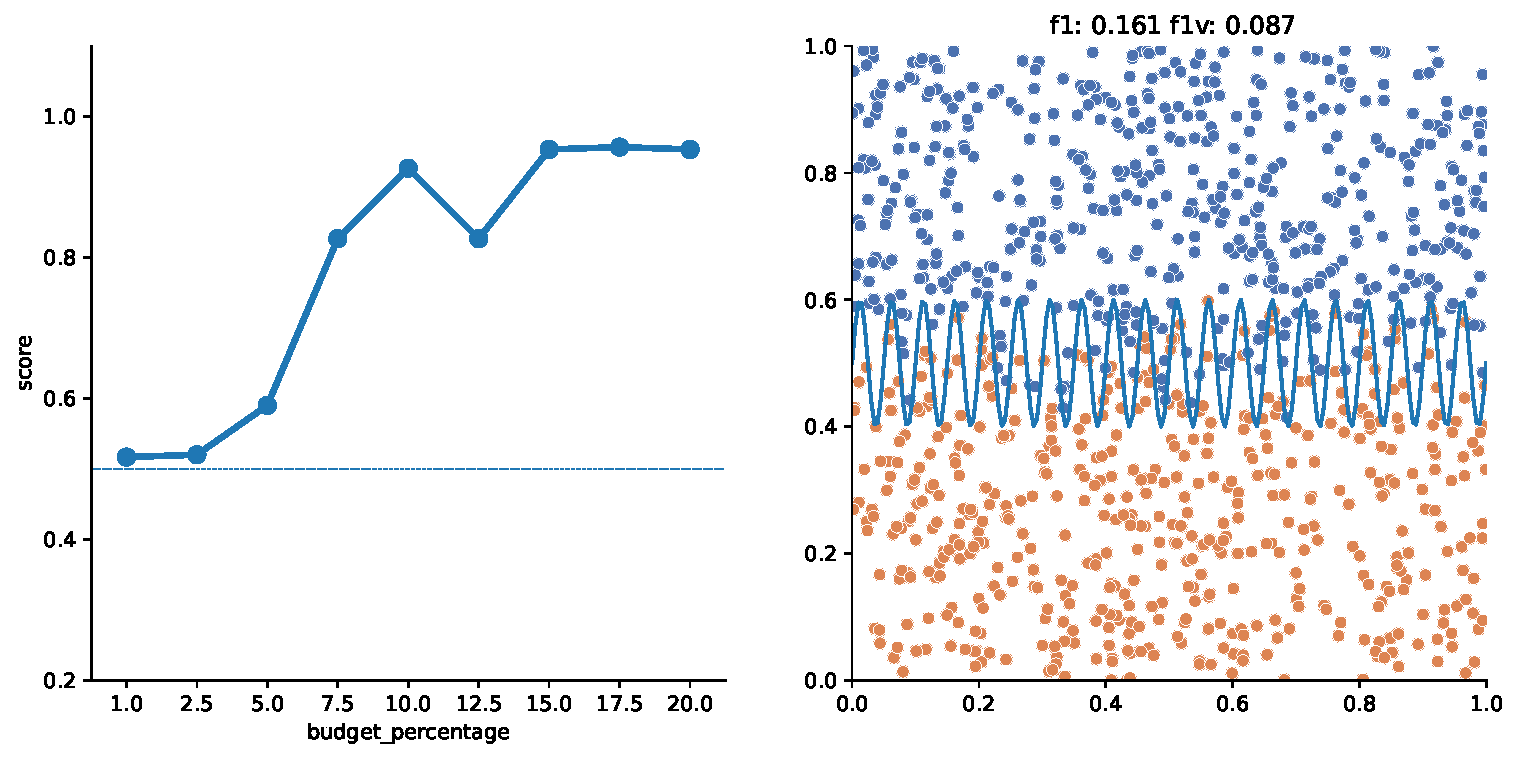
\includegraphics[width=\textwidth]{img/2d_v2/14.pdf}
    \end{subfigure}
    \begin{subfigure}{.5\textwidth}
        \centering
        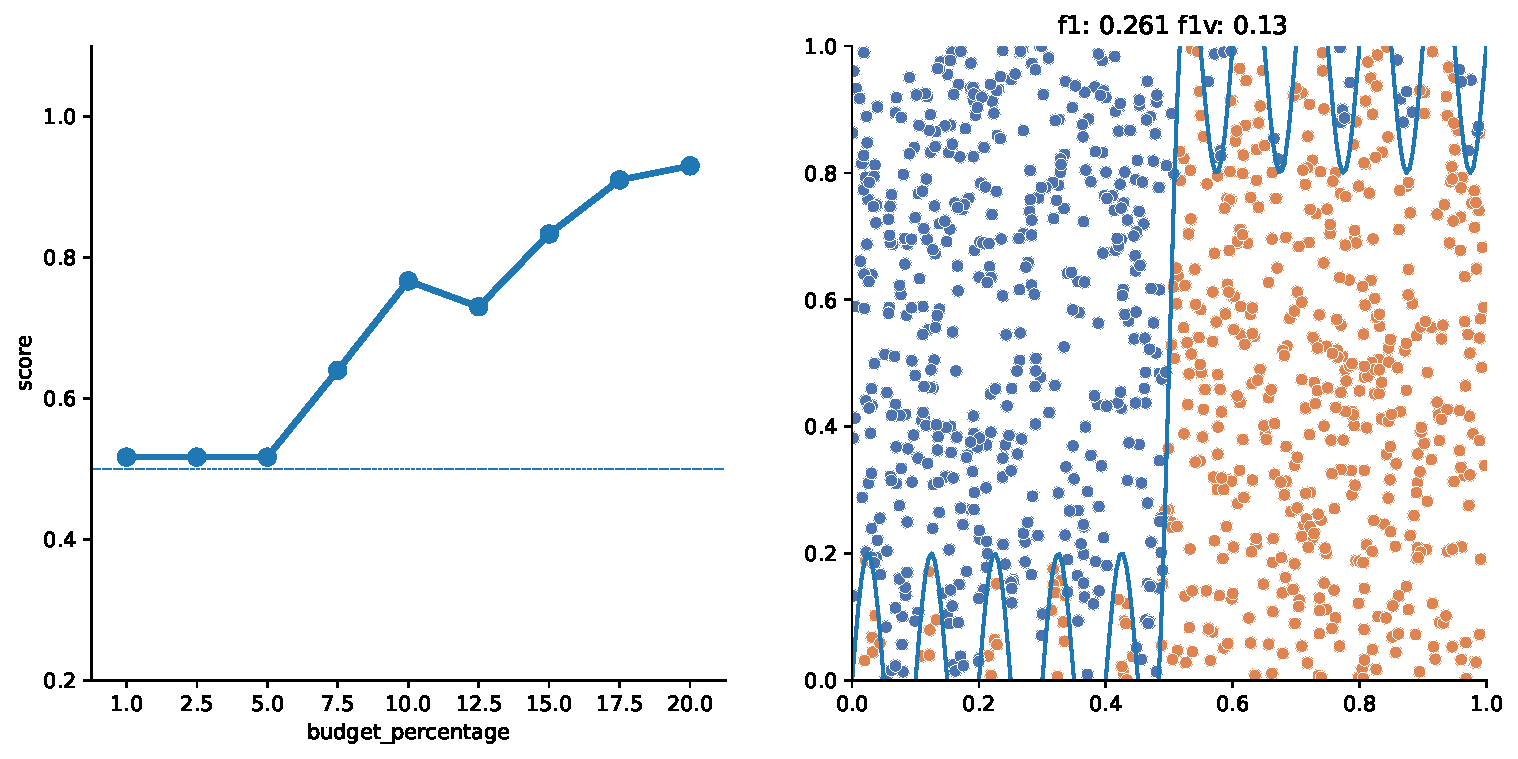
\includegraphics[width=\textwidth]{img/2d_v2/15.pdf}
    \end{subfigure}%
\caption[Risultati su \emph{dataset} sintetici utilizzando la strategia 2.]{Risultati più significativi ottenuti su \emph{dataset} sintetici 2D utilizzando la strategia 2. Ognuno dei grafici a sinistra indica l'andamento dell'accuratezza sui dati di \emph{test} al variare del \emph{budget}; ognuno dei grafici a destra rappresenta il \emph{dataset} utilizzato con le rispettive metriche di difficoltà.}
\label{fig:2d_v2}
\end{figure}
Dai risultati ottenuti si può notare come anche per la maggior parte dei \emph{dataset} difficili sia possibile utilizzare un \emph{budget} stringente, tra il $7\%$ e il $10\%$, con perdite accettabili di accuratezza.
Questo comportamento è in linea con le osservazioni fatte per l'esperimento precedente, dove per valori di \emph{budget} stringenti ($30\%$ per la strategia 1, che ricade nella maggior parte dei casi nell'intervallo $7\%-15\%$ della strategia 2) la perdita di accuratezza riscontrata non è così marcata.

Su \emph{dataset} per cui una superficie di separazione lineare approssima in modo soddisfacente la funzione di etichettatura originale, la riduzione di \emph{budget} può essere molto importante: anche con \emph{budget} pari all'$1\%$ della dimensione del \emph{dataset} si ottiene un'accuratezza pari a quella ottenuta con \emph{budget} molto più alti.

In generale, è possibile identificare per ogni \emph{dataset} un valore soglia di \emph{budget} per cui l'accuratezza è simile a quella ottenuta con valori di \emph{budget} più alti. 
L'accuratezza invece ottenuta con valori di \emph{budget} minori del valore soglia diminuisce significativamente al diminuire del \emph{budget}.
\section{Esperimenti su dataset sintetici 3D}\label{sec:exp:synth_3d}
Una piccola parte degli esperimenti è stata effettuata su \emph{dataset} in tre dimensioni generati con la funzione di etichettatura paraboloide.
Questi \emph{dataset} sono composti da 5600 elementi di addestramento e da 2400 di \emph{test}.
In~\Cref{fig:3d_exp} si visualizza l'andamento dell'accuratezza e dello \emph{score ratio} al variare del \emph{budget}.
\begin{figure}
    \begin{subfigure}{\textwidth}
        \centering
        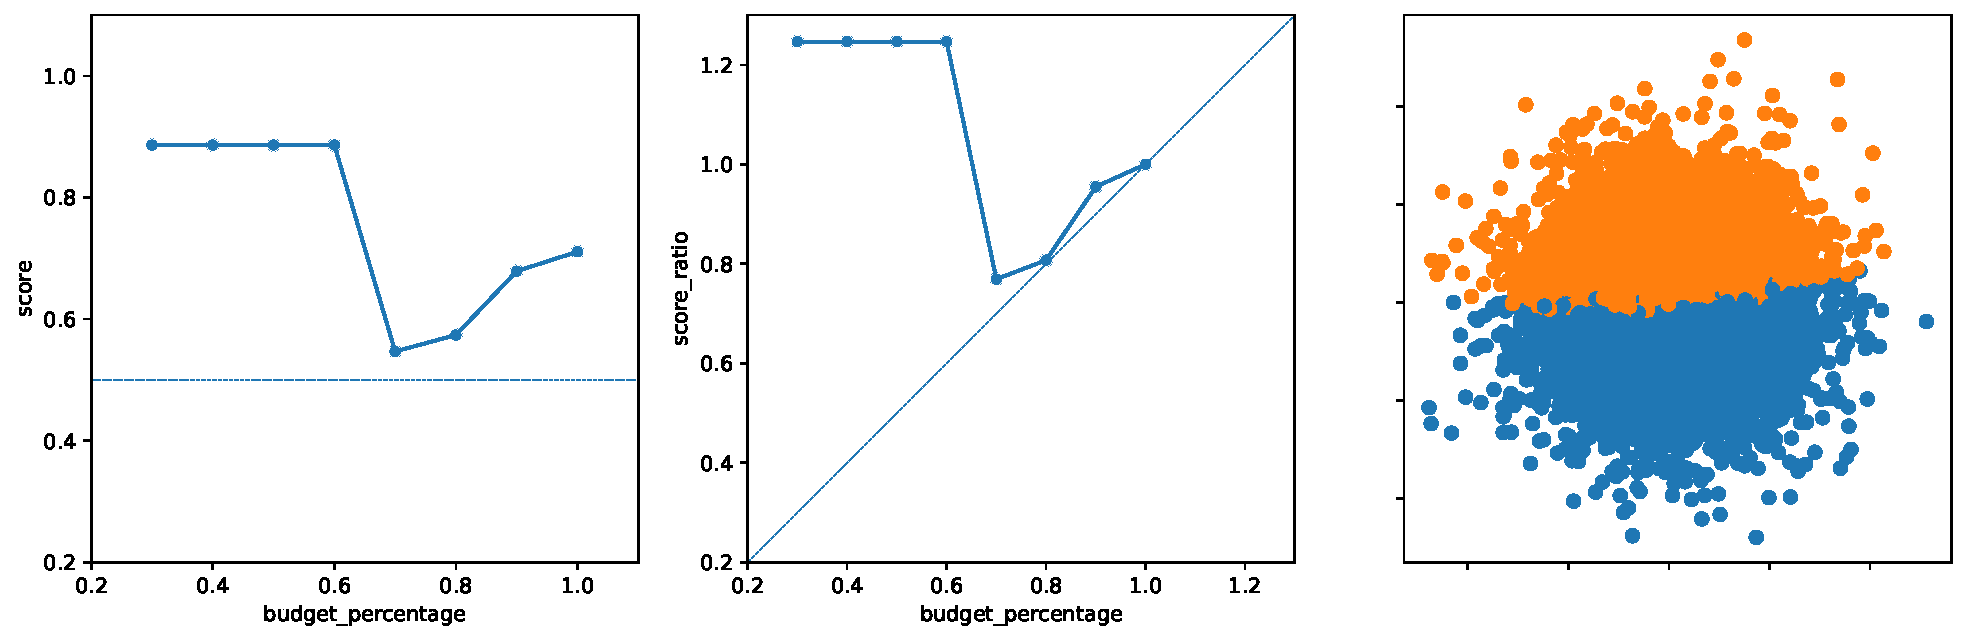
\includegraphics[width=\textwidth]{img/3d/1.pdf}
    \end{subfigure}%
    \hfill
    \begin{subfigure}{\textwidth}
        \centering
        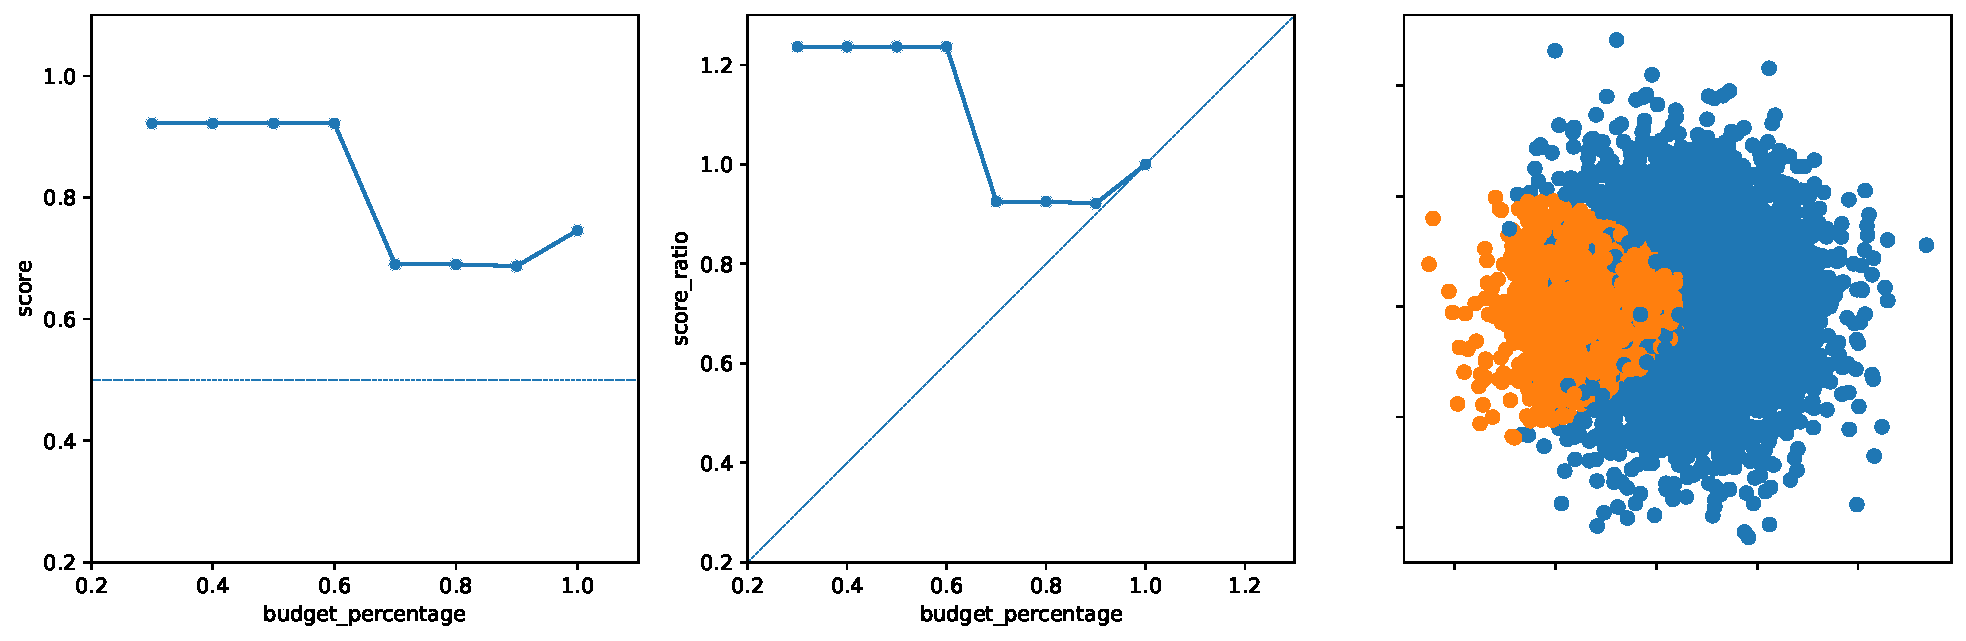
\includegraphics[width=\textwidth]{img/3d/2.pdf}
    \end{subfigure}%
    \hfill
    \begin{subfigure}{\textwidth}
        \centering
        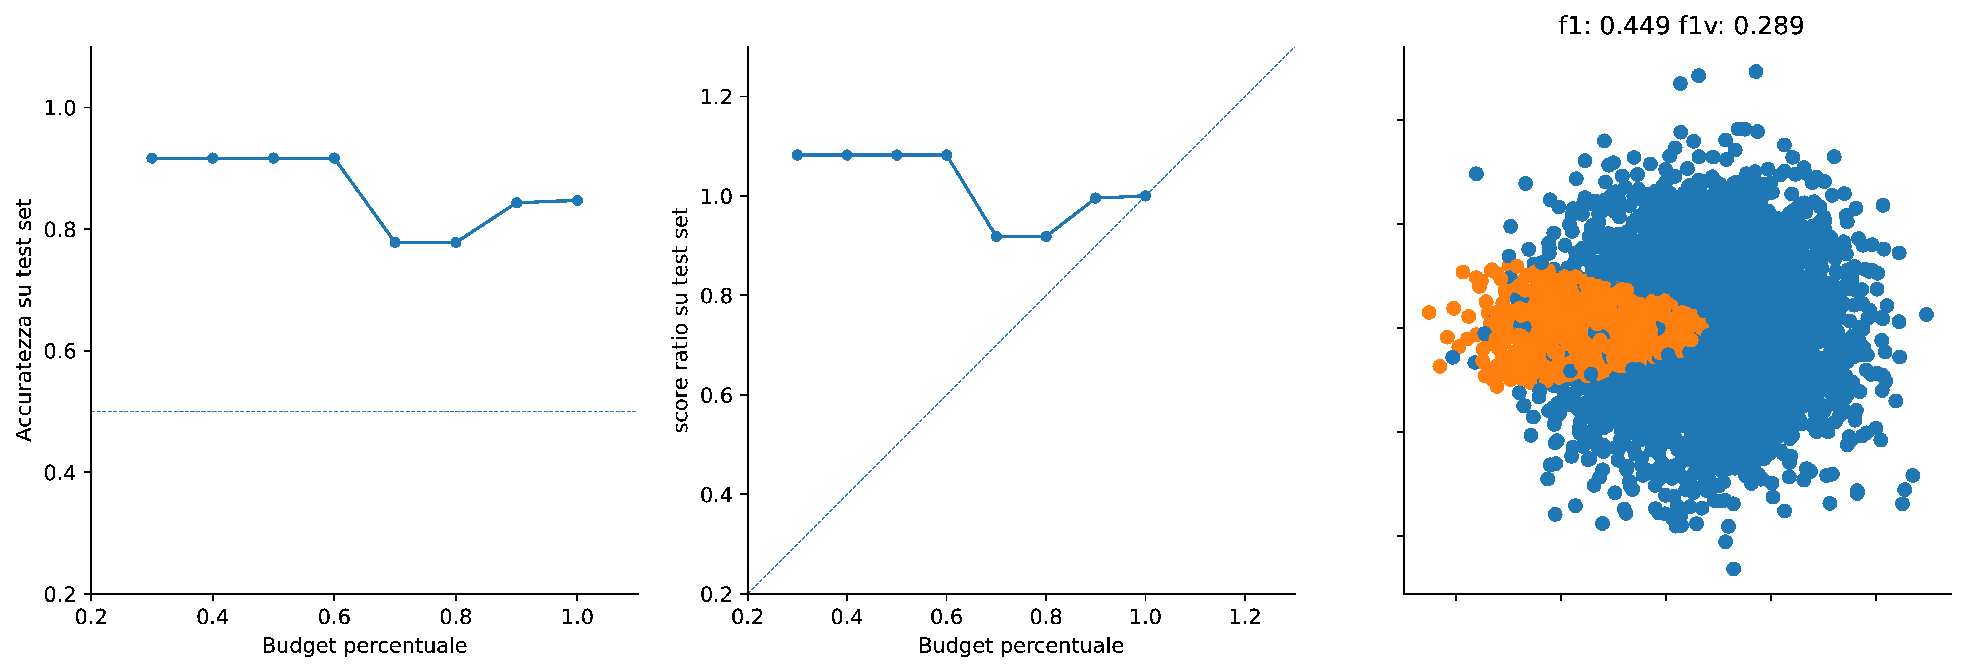
\includegraphics[width=\textwidth]{img/3d/3.pdf}
    \end{subfigure}%
\caption{Esperimenti su \emph{dataset} sintetici 3D utilizzando la strategia 1. A sinistra l'accuratezza sui dati di test al variare del \emph{budget}; al centro lo ``score ratio'' al variare del \emph{budget}; a destra il \emph{dataset} ridotto a due dimensioni utilizzando \emph{principal component analysis}.}
\label{fig:3d_exp}
\end{figure}
Dai risultati ottenuti si nota che per valori di \emph{budget} alti ($80/90\%$) l'andamento dei valori misurati sia in linea con le aspettative, calando proporzionalmente alla riduzione di \emph{budget}.
Tuttavia, l'accuratezza dei modelli con \emph{budget} più ristretti sale fino a superare l'accuratezza dei modelli classici, abbastanza bassa in termini assoluti.
Inoltre, i modelli classici utilizzano una quantità di vettori di supporto molto vicina alla dimensione dell'intero insieme di addestramento.
Questo comportamento è inatteso e meriterebbe un approfondimento futuro, non eseguito in questa tesi a causa dell'elevato tempo di calcolo richiesto per addestrare e selezionare i modelli.

\section{Esperimenti su dataset di terze parti}\label{sec:exp:real_ds}
Utilizzando i \emph{dataset} descritti nella~\Cref{tab:uci_datasets} sono stati effettuati degli esperimenti con le diverse strategie.

I risultati ottenuti utilizzando la strategia 1 sono illustrati in~\Cref{fig:TP_old_strategy}.
\begin{figure}
    \centering
    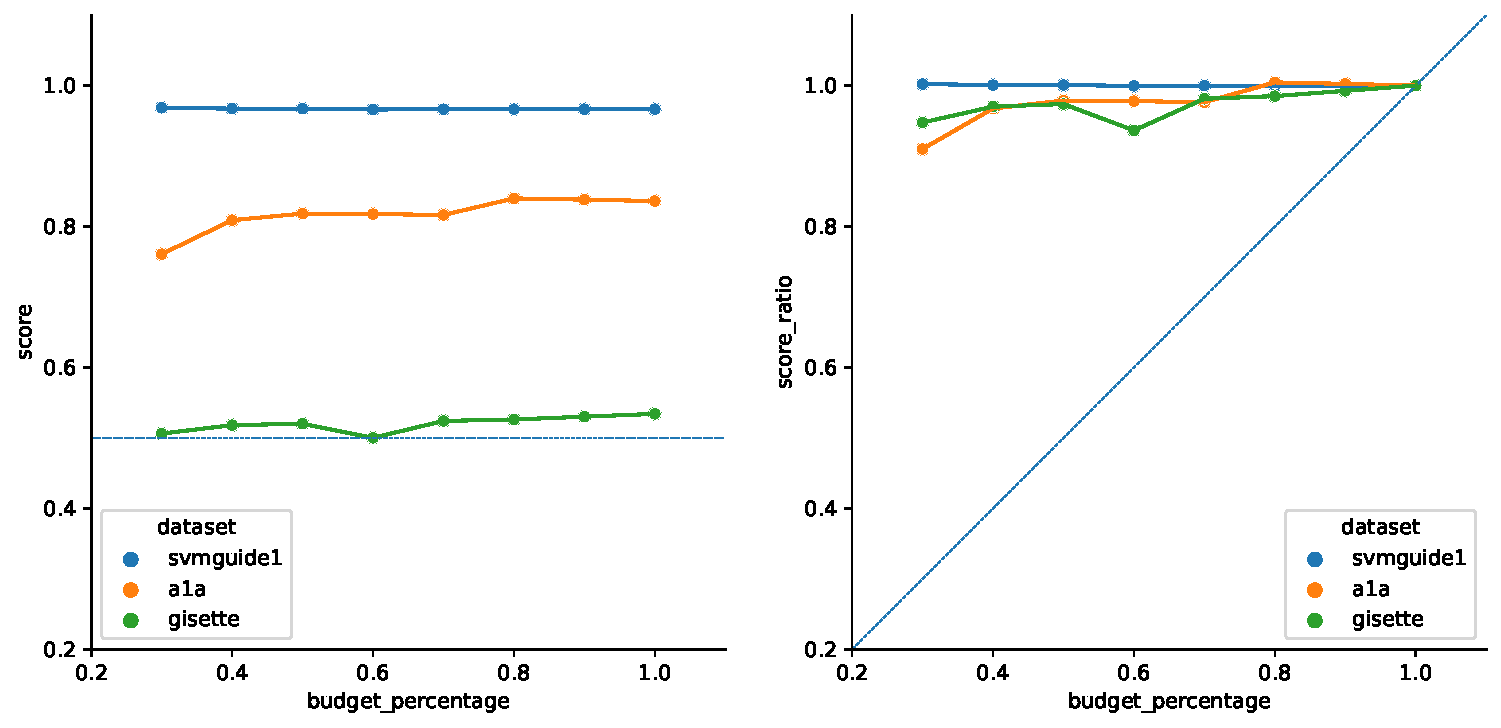
\includegraphics[width=1\linewidth]{img//TP/tp_old_strategy.pdf}
    \caption[Risultati degli esperimenti su \emph{dataset} di terze parti utilizzando la strategia 1.]{Risultati esperimenti su \emph{dataset} di terze parti utilizzando la strategia 1. A sinistra l'accuratezza sui dati di test al variare del \emph{budget}; a destra lo \emph{score ratio} al variare del \emph{budget}.}
    \label{fig:TP_old_strategy}
\end{figure}
Si può notare come su questi \emph{dataset} tutte le riduzioni di \emph{budget} utilizzate siano efficaci e non risultino in perdite di accuratezza significative: ogni modello \emph{budgeted SVC} è sostanzialmente equivalente come bontà al rispettivo modello classico.
L'accuratezza ottenuta sul \emph{dataset gisette} indica come nessuno dei modelli prodotti sia efficace a modellare quel problema; questo risultato non è preoccupante perché le caratteristiche di questi dati rendono il problema particolarmente difficile: questo \emph{dataset} è di dimensione modesta (6000 elementi di addestramento) rispetto al numero degli attributi (5000).

I risultati ottenuti utilizzando la strategia 2 sono illustrati in~\Cref{fig:TP_new_strategy}.
\begin{figure}
    \centering
    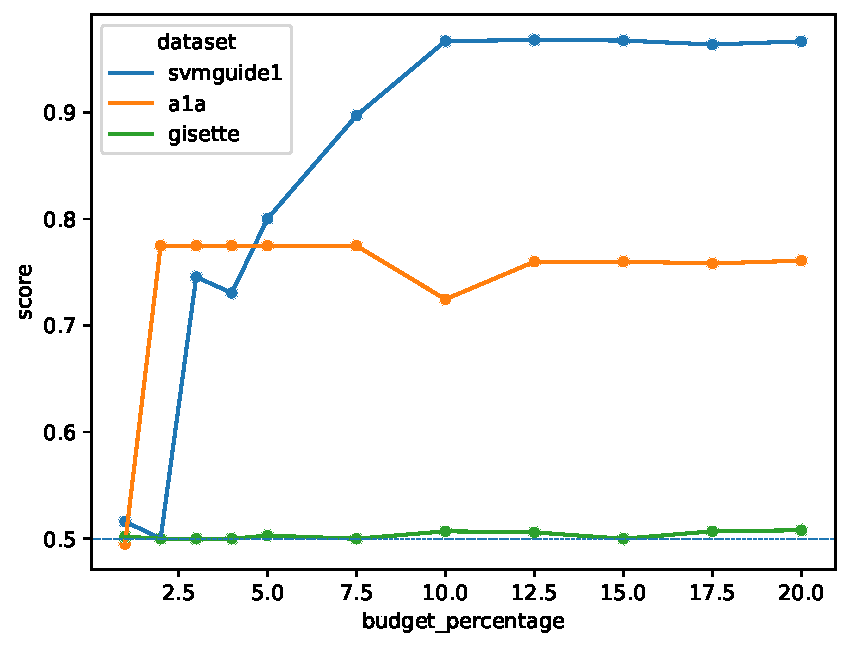
\includegraphics[width=0.5\linewidth]{img//TP/tp_new_strategy.pdf}
    \caption[Risultati su \emph{dataset} di terze parti utilizzando la strategia 2.]{Accuratezza al variare del \emph{budget} sui \emph{dataset} di terze parti utilizzando la strategia 2.}
    \label{fig:TP_new_strategy}
\end{figure}
Così come per gli analoghi esperimenti effettuati su \emph{dataset} sintetici, è possibile notare come per ogni \emph{dataset} sia possibile identificare un valore soglia di \emph{budget} che divide \emph{budget} non penalizzanti da \emph{budget} penalizzanti.

\section{Confronto con altri metodi}\label{sec:comparazione_metodi}
Per meglio inquadrare i risultati ottenuti dal metodo \emph{budgeted SVC}, sono stati ripetuti gli esperimenti descritti in precedenza utilizzando delle implementazioni di metodi proposti in letteratura e descritti nel~\Cref{chap:sparse_svc}, in particolare:
\begin{itemize}
    \item \emph{BSGD SVM}~\cite{2012_bsgd}, risolutore pensato per addestramento \emph{on-line} basato su discesa del gradiente che mantiene una dimensione massima dell'insieme dei vettori di supporto utilizzando la strategia di unione o rimozione;
    \item \emph{NSSVM}~\cite{2020_sparse_svm}, risolutore basato su \emph{Newton method} che minimizza il numero di vettori di supporto tramite una funzione di costo adeguata.
    % \item \emph{LIB IRWLS} esposto in~\cite{LIBIRWLS}. Risolutore parallelo basato su un approssimazione \emph{greedy} della matrice \emph{kernel} e utilizzo dell'algoritmo IRWLS~\cite{IRWLS}
\end{itemize}
Utilizzando gli stessi \emph{dataset} sintetici generati con i parametri nelle~\Cref{tab:parametri_ds_sin,tab:parametri_ds_pacman} e utilizzando \emph{5-fold cross-validation} con una ricerca esaustiva sulla griglia di parametri adatti descritta in~\Cref{tab:gridsearch_comparazioni}, viene misurata l'accuratezza sui dati di \emph{test} per gli stessi valori di \emph{budget} utilizzati negli esperimenti precedenti.
\begin{table}
    \centering
    \begin{tabular}{ccccc}
        \toprule
        Algoritmo & $C$ & \emph{Kernel} & $\gamma$ & d \\
        \midrule
        \multirow{2}{*}{BSGD}   & \multirow{2}{*}{/}  & Gaussiano   & [0.001, 0.01, 0.1, 1, 10]   & /\\
                                      \cline{3-5}
                                &   & Polinomiale & / & [2, 5, 10] \\
        \hline
        NSSVM   & / & / & / & / \\
        % \hline
        % IRWLS   & [0.01, 0.1, 1, 10]  & Gaussiano & [0.001, 0.01, 0.1, 1, 10] & / \\
        \bottomrule
    \end{tabular}
    \caption{Parametri \emph{grid search} per gli algoritmi presenti in letteratura.}
    \label{tab:gridsearch_comparazioni}
\end{table}
In~\Cref{fig:comp_old} si possono vedere i risultati ottenuti utilizzando la strategia 1, mentre in~\Cref{fig:comp_new} si possono vedere i risultati ottenuti utilizzando la strategia 2.
Come per gli esperimenti precedenti, queste figure riportano i risultati più significativi, mentre i restanti grafici sono inseriti nell'Appendice A.
\begin{figure}
    \begin{subfigure}{.5\textwidth}
        \centering
        \includegraphics[width=\textwidth]{img/comp_old/3.pdf}
    \end{subfigure}%
    \begin{subfigure}{.5\textwidth}
        \centering
        \includegraphics[width=\textwidth]{img/comp_old/4.pdf}
    \end{subfigure}
    %
    \hfill
    %
    \begin{subfigure}{.5\textwidth}
        \centering
        \includegraphics[width=\textwidth]{img/comp_old/8.pdf}
    \end{subfigure}
    \begin{subfigure}{.5\textwidth}
        \centering
        \includegraphics[width=\textwidth]{img/comp_old/9.pdf}
    \end{subfigure}%
    %
    \hfill
    %
    \begin{subfigure}{.5\textwidth}
        \centering
        \includegraphics[width=\textwidth]{img/comp_old/10.pdf}
    \end{subfigure}
    \begin{subfigure}{.5\textwidth}
        \centering
        \includegraphics[width=\textwidth]{img/comp_old/12.pdf}
    \end{subfigure}%
    %
    \hfill
    %
    \begin{subfigure}{.5\textwidth}
        \centering
        \includegraphics[width=\textwidth]{img/comp_old/13.pdf}
    \end{subfigure}
    \begin{subfigure}{.5\textwidth}
        \centering
        \includegraphics[width=\textwidth]{img/comp_old/14.pdf}
    \end{subfigure}
        %
    \hfill
    %
    \begin{subfigure}{.5\textwidth}
        \centering
        \includegraphics[width=\textwidth]{img/comp_old/15.pdf}
    \end{subfigure}
\caption[Risultati su \emph{dataset} sintetici utilizzando strategia 1 in confronto ad altri metodi.]{Risultati più significativi ottenuti su \emph{dataset} sintetici 2D utilizzando la strategia 1, analogo ai risultati in~\Cref{fig:risultati_2d} ma con una curva per ogni metodo utilizzato: la proposta \emph{Budgeted SVC}, i metodi \emph{NSSVM} e \emph{BSGD}.}
\label{fig:comp_old}
\end{figure}
Confrontando i risultati ottenuti con la strategia 1, è possibile notare come anche i modelli prodotti dagli altri metodi, con frequenza minore, risultino in valori di accuratezza molto vari per i diversi \emph{dataset} generati con seme diverso.
Allo stesso tempo, escludendo pochi casi anomali, la perdita di accuratezza al variare di \emph{budget} ottenuta da questi metodi sembra essere più lineare rispetto alla proposta \emph{budgeted SVC}.
\begin{figure}
    \begin{subfigure}{.5\textwidth}
        \centering
        \includegraphics[width=\textwidth]{img/comp_new/4.pdf}
    \end{subfigure}%
    \begin{subfigure}{.5\textwidth}
        \centering
        \includegraphics[width=\textwidth]{img/comp_new/5.pdf}
    \end{subfigure}
    %
    \hfill
    %
    \begin{subfigure}{.5\textwidth}
        \centering
        \includegraphics[width=\textwidth]{img/comp_new/7.pdf}
    \end{subfigure}
    \begin{subfigure}{.5\textwidth}
        \centering
        \includegraphics[width=\textwidth]{img/comp_new/8.pdf}
    \end{subfigure}%
    %
    \hfill
    %
    \begin{subfigure}{.5\textwidth}
        \centering
        \includegraphics[width=\textwidth]{img/comp_new/12.pdf}
    \end{subfigure}
    \begin{subfigure}{.5\textwidth}
        \centering
        \includegraphics[width=\textwidth]{img/comp_new/13.pdf}
    \end{subfigure}%
    %
    \hfill
    %
    \begin{subfigure}{.5\textwidth}
        \centering
        \includegraphics[width=\textwidth]{img/comp_new/14.pdf}
    \end{subfigure}
    \begin{subfigure}{.5\textwidth}
        \centering
        \includegraphics[width=\textwidth]{img/comp_new/15.pdf}
    \end{subfigure}
\caption[Risultati su \emph{dataset} sintetici utilizzando strategia 2 in confronto ad altri metodi.]{Risultati più significativi ottenuti su \emph{dataset} sintetici 2D utilizzando la strategia 2, analogo ai risultati in~\Cref{fig:2d_v2} ma con una curva per ogni metodo utilizzato: la proposta \emph{Budgeted SVC}, i metodi \emph{NSSVM} e \emph{BSGD}.}
\label{fig:comp_new}
\end{figure}
Confrontando i risultati ottenuti con la strategia 2, si può notare come i modelli prodotti dalla formulazione \emph{budgeted SVC} siano competitivi per valori di \emph{budget} alti e come siano invece peggiori per valori di \emph{budget} bassi. 
La perdita di accuratezza dovuta alla restrizione di \emph{budget} si manifesta per \emph{budgeted SVC} con valori di \emph{budget} più alti rispetto agli altri metodi.

\section{Memorizzazione compressa dei modelli SVC}\label{sec:memorizzazione_compressa}
Un ulteriore metodo per diminuire lo spazio di memorizzazione richiesto per un modello SVC si basa sull'osservazione che, nella formulazione \emph{soft margin}, i moltiplicatori $\alpha_i$ sono al più grandi quanto $C$, e non è quindi necessario memorizzare tutti i moltiplicatori $\alpha_i = C$.

Assumendo che le etichette positive abbiano valore $+1$ e le etichette negative abbiano valore $-1$ (e considerando che si può sempre forzare questa assunzione a essere vera), si definiscono i valori:
\begin{itemize}
    \item $s^+ = |\{\alpha_i, i=1,\dots,m : 0 < \alpha_i < C, y_i=+1\}|$, numero di moltiplicatori con valore compreso in $(0, C)$ e con etichetta appartenente alla classe positiva;
    \item $s^- = |\{\alpha_i, i=1,\dots,m : 0 < \alpha_i < C, y_i=-1\}|$, numero di moltiplicatori con valore compreso in $(0, C)$ e con etichetta appartenente alla classe negativa;
    \item $b^+ = |\{\alpha_i, i=1,\dots,m : \alpha_i = C, y_i=+1\}|$, numero di moltiplicatori con valore uguale a $C$ e con etichetta appartenente alla classe positiva;
    \item $b^- = |\{\alpha_i, i=1,\dots,m : \alpha_i = C, y_i=-1\}|$, numero di moltiplicatori con valore uguale a $C$ e con etichetta appartenente alla classe negativa.
\end{itemize}
Si ipotizzi quindi di memorizzare i vettori di supporto in gruppi contigui in base alla valore dei corrispettivi moltiplicatori, utilizzando l'ordinamento rappresentato in~\Cref{fig:schema_memorizzazione_sv}.
\begin{figure}
    \centering
    \includegraphics{img/memorizzazione_sv.pdf}
    \caption{Esempio di memorizzazione ordinata dei vettori di supporto. Ogni gruppo (identificato da un rettangolo) contiene vettori di supporto i quali moltiplicatori appartengono alla stessa categoria.}
    \label{fig:schema_memorizzazione_sv}
\end{figure}
Utilizzando questa memorizzazione compressa, l'originale calcolo di una nuova predizione per il punto $\Vec{x}_{\text{test}}$
\begin{equation*}
    h(\Vec{x}_{\text{test}}) = \sign\left(\sum_{i \in S}\alpha_i^*y_iK(\Vec{x}_i, \Vec{x}_\text{test}) + b^*\right),
\end{equation*}
visto nel~\Cref{sec:kernel_trick}, può essere trasformato in
\begin{align*}
    h(\Vec{x}_{\text{test}}) = \sign\bigg(
            \sum_{i=1}^{s^+}\alpha_i^*K(\Vec{x}_i, \Vec{x}_\text{test}) 
            -\sum_{i=s^++1}^{s^-}\alpha_i^*K(\Vec{x}_i, \Vec{x}_\text{test})\\
            +C\sum_{i=s^-+1}^{b^+}K(\Vec{x}_i, \Vec{x}_\text{test})
            -C\sum_{i=b^++1}^{b^-}K(\Vec{x}_i, \Vec{x}_\text{test}) 
            + b^*
        \bigg).
\end{align*}
Si può notare come questa rappresentazione compressa sia vantaggiosa in termini di spazio, perché non richiede di memorizzare tutti i moltiplicatori lagrangiani con valore uguale a $C$.
D'altra parte, si complica leggermente la realizzazione pratica del modello.
In~\Cref{tab:compressione_spazio_risparmiato} si confrontano i requisiti di spazio per una memorizzazione classica e la memorizzazione compressa.
\begin{table}
    \centering
    \begin{tabular}{c|c|c}
    \multicolumn{1}{c}{}    &  Memorizzazione Classica    & Memorizzazione Compressa \\     
    \toprule
    Numero di moltiplicatori    & $s^+ + s^- + b^+ + b^-$ & $s^+ +s^-$ \\
    \hline
    Numero di etichette         & $s^+ + s^- + b^+ + b^-$ &  / \\
    \hline
    Altre variabili             &         $b^*$          &  $s^+, s^-, b^+, b^-, C, b^*$ \\
    \bottomrule
    \end{tabular}
    \caption{Requisiti di spazio della memorizzazione classica e delle memorizzazione compressa.}
    \label{tab:compressione_spazio_risparmiato}
\end{table}
Come si può notare, la memorizzazione compressa consente di evitare di memorizzare $b^++b^-$ moltiplicatori rispetto alla memorizzazione classica.
Ipotizzando che i moltiplicatori siano variabili \emph{float} da quattro \emph{byte} ciascuna, si possono risparmiare $4(b^++b^-)$ \emph{byte} relativamente ai moltiplicatori lagrangiani e $4(s^+ + s^- + b^+ + b^-)$ relativamente alle etichette, ma sono richieste cinque variabili intere aggiuntive per memorizzare $s^+, s^-, b^+, b^-, C$.
La memorizzazione compressa è praticamente sempre conveniente in termini di spazio, ed è tanto più conveniente quanto la quantità $b^++b^-$ è grande.

Per avere delle indicazioni di quanto spazio si possa risparmiare utilizzando questa rappresentazione, si mostrano nelle~\Cref{fig:dist_riduzione_synth_old,fig:dist_riduzione_synth_new} le distribuzioni delle potenziali riduzioni in spazio richiesto per memorizzare gli indici per gli esperimenti su \emph{dataset} sintetici descritti nel~\Cref{sec:exp:synth_2d} e si mostrano nelle~\Cref{fig:dist_riduzione_TP_old,fig:dist_riduzione_TP_new} le distribuzioni delle potenziali riduzioni in spazio richiesto per memorizzare gli indici per gli esperimenti su \emph{dataset} di terze parti descritti nel~\Cref{sec:exp:real_ds}.
\begin{figure}
    \centering
    \includegraphics[width=.7\linewidth]{img/decremento_spazio_indici_exp2d_old.pdf}
    \caption{Distribuzioni, per percentuale di \emph{budget}, della riduzione dello spazio richiesto per memorizzare gli indici, relativamente agli esperimenti su \emph{dataset} sintetici effettuati con strategia 1.}
    \label{fig:dist_riduzione_synth_old}
\end{figure}%
\begin{figure}
    \centering
    \includegraphics[width=.7\linewidth]{img/decremento_spazio_indici_exp2d_new.pdf}
    \caption{Distribuzioni, per percentuale di \emph{budget}, della riduzione dello spazio richiesto per memorizzare gli indici, relativamente agli esperimenti su \emph{dataset} sintetici effettuati con strategia 2.}
    \label{fig:dist_riduzione_synth_new}
\end{figure}
\begin{figure}
    \centering
    \includegraphics[width=.7\linewidth]{img/decremento_spazio_indici_TP_old.pdf}
    \caption{Distribuzioni, per percentuale di \emph{budget}, della riduzione dello spazio richiesto per memorizzare gli indici, relativamente agli esperimenti su \emph{dataset} di terze parti effettuati con strategia 1.}
    \label{fig:dist_riduzione_TP_old}
\end{figure}%
\begin{figure}
    \centering
    \includegraphics[width=.7\linewidth]{img/decremento_spazio_indici_TP_new.pdf}
    \caption{Distribuzioni, per percentuale di \emph{budget}, della riduzione dello spazio richiesto per memorizzare gli indici, relativamente agli esperimenti su \emph{dataset} di terze parti effettuati con strategia 2.}
    \label{fig:dist_riduzione_TP_new}
\end{figure}
Molti dei modelli prodotti con gli esperimenti su \emph{dataset} di terze parti beneficerebbero di una riduzione significativa nel numero di indici da memorizzare, mentre per i modelli prodotti su \emph{dataset} sintetici, è meno frequente il caso di un risparmio importante in termini di spazio.

\backmatter
    \chapter{Conclusioni e sviluppi futuri}
\label{chap:conclusioni}
In questa tesi è stato proposto L'approccio \emph{budgeted SVC} per addestrare classificatori con un ristretto numero di vettori di supporto.
Gli esperimenti effettuati su diversi \emph{dataset} sintetici evidenziano come il metodo sia promettente. 
Le motivazioni sono esposte nell'elenco seguente.
\begin{itemize}
    \item Per alcuni \emph{dataset} facili, la riduzione in termini di spazio può essere significativa e non penalizzate in termini di accuratezza.
    \item Per altri \emph{dataset} difficili, l'accuratezza subisce un peggioramento significativo al diminuire del \emph{budget}, fino al punto in cui per riduzioni importanti l'accuratezza ritorna ad essere buona.
    \item Esprimendo il budget come percentuale della dimensione del \emph{dataset}, si nota come valori tra il $5\%$ ed il $7\%$ possano essere delle buone scelte per risparmiare spazio senza sacrificare troppo in termini di efficacia.
\end{itemize}

Gli esperimenti effettuati su \emph{dataset} di terze parti sono anche più promettenti dei precedenti risultati:
\begin{itemize}
    \item utilizzando la strategia 1, tutti i modelli con \emph{budget} esibiscono la stessa accuratezza del corrispettivo modello classico;
    \item utilizzando la strategia 2, si evidenzia come la perdita in accuratezza sia proporzionale alla riduzione di \emph{budget}.
\end{itemize}


Il confronto con altri metodi evidenzia come \emph{budgeted SVC}..................


Il lavoro iniziato in questa tesi potrebbe sicuramente essere sviluppato ulteriormente, cercando di espandere o migliorare alcuni aspetti, elencati di seguito.
\begin{itemize}
    \item Si potrebbe verificare se la variabilità ottenuta su diversi \emph{dataset} generati con gli stessi parametri sia effettivamente dovuta al fatto che il risolutore non fornisca una soluzione ottima. 
    \item Si potrebbero utilizzare \emph{dataset} sintetici di dimensione maggiore e/o \emph{dataset} con un più alto numero di feature. Si potrebbero utilizzare ulteriori \emph{dataset} di terze parti con caratteristiche diverse rispetto a quelli già considerati.
    \item Si potrebbero proporre ulteriori indicazioni o dei criteri più solidi per come impostare dei valori di budget a priori, per esempio in base alle caratteristiche dei dati disponibili.
    \item Si potrebbero incorporare delle proposte presentate in letteratura, per esempio per limitare l'effetto del rumore o per rendere il problema trattabile con altri metodi risolutivi.
    \item Si potrebbe investigare un eventuale relazione tra \emph{budget} e rumore, per capire se una quantità molto stringente di \emph{budget} corrisponda ad una maggior robustezza rispetto a dati erroneamente etichettati.
\end{itemize}



\bibliographystyle{unsrt}
\bibliography{bibliografia}
\addcontentsline{toc}{chapter}{Bibliografia}


% \appendix\label{appendix:2d_old}
% \appendixpage
% \addappheadtotoc

\begin{appendices}
\chapter*{Appendice}\label{appendix}
\section*{Grafici omessi nel~\Cref{chap:esperimenti}}
\begin{figure}[!ht]
    \begin{subfigure}{.4999\textwidth}
        \centering
        \includegraphics[width=\textwidth]{img/2d/1.pdf}
    \end{subfigure}%
    \begin{subfigure}{.5\textwidth}
        \centering
        \includegraphics[width=\textwidth]{img/2d/2.pdf}
    \end{subfigure}%
    %
    \hfill
    %
    \begin{subfigure}{.5\textwidth}
        \centering
        \includegraphics[width=\textwidth]{img/2d/5.pdf}
    \end{subfigure}%
    \begin{subfigure}{.5\textwidth}
        \centering
        \includegraphics[width=\textwidth]{img/2d/6.pdf}
    \end{subfigure}%
    %
    \hfill
    %
    \begin{subfigure}{.5\textwidth}
        \centering
        \includegraphics[width=\textwidth]{img/2d/7.pdf}
    \end{subfigure}%
    \begin{subfigure}{.5\textwidth}
        \centering
        \includegraphics[width=\textwidth]{img/2d/11.pdf}
    \end{subfigure}%
    \caption{Questi grafici completano la~\Cref{fig:risultati_2d}.}
\end{figure}

\begin{figure}
    \begin{subfigure}{.5\textwidth}
        \centering
        \includegraphics[width=\textwidth]{img/2d_v2/1.pdf}
    \end{subfigure}%
    \begin{subfigure}{.5\textwidth}
        \centering
        \includegraphics[width=\textwidth]{img/2d_v2/2.pdf}
    \end{subfigure}
    %
    \hfill
    %
    \begin{subfigure}{.5\textwidth}
        \centering
        \includegraphics[width=\textwidth]{img/2d_v2/3.pdf}
    \end{subfigure}
    \begin{subfigure}{.5\textwidth}
        \centering
        \includegraphics[width=\textwidth]{img/2d_v2/6.pdf}
    \end{subfigure}%
    %
    \hfill
    %
    \begin{subfigure}{.5\textwidth}
        \centering
        \includegraphics[width=\textwidth]{img/2d_v2/9.pdf}
    \end{subfigure}
    \begin{subfigure}{.5\textwidth}
        \centering
        \includegraphics[width=\textwidth]{img/2d_v2/10.pdf}
    \end{subfigure}%
    %
    \hfill
    %
    \begin{subfigure}{.5\textwidth}
        \centering
        \includegraphics[width=\textwidth]{img/2d_v2/11.pdf}
    \end{subfigure}
\caption{Questi grafici completano la~\Cref{fig:2d_v2}.}
\end{figure}

\end{appendices}

\end{document}


 
